\documentclass[phd,black]{PrincetonThesis}
\usepackage{hyperref}
\usepackage{hepnames}
\usepackage{multirow}
\usepackage{epsfig}
\usepackage{subfigure}
\usepackage{slashed}
\usepackage{amssymb}
\usepackage{array}
\usepackage{fp}
\usepackage{acronym} %texorpdfstring
\usepackage{ifthen}
\usepackage{ptdr-definitions}

\newcolumntype{T}{>{\trunc}r}
\def\trunc\ignorespaces#1\\{%
  \FPset\a{#1}
  \FPround\a\a4
  \a
  \\
}

%  Needed to insert AN-12-402 in to thesis.
\newboolean{cms@an}
\setboolean{cms@an}{true} 

%\newcommand{\registered}{\ooalign{\hfil\raise .00ex\hbox{\scriptsize R}\hfil\crcr\mathhexbox20D} }
\newcommand{\lt}{\!<\! }
\newcommand{\gt}{\!>\! }
\newcommand{\instLumiUnit}{cm$^{-2}$s$^{-1}$ }
\newcommand{\CHECK}[1]{\textbf{\color{red}[#1]}\xspace }
\newcommand{\chk}[1]{\CHECK{CHECK THIS!} }

%\ from AN-12-402
\newcommand{\cmsSymbolFace}{\mathrm}
\newcommand{\X}{\ensuremath{\mathrm{X^{0}}}\xspace}
\newcommand{\XX}{\ensuremath{\mathrm{X^{0}X^{0}}}\xspace}
\newcommand{\BR}{\ensuremath{\mathrm{B}}\xspace}
\newcommand{\Higgs}{\Hz}
\newcommand{\Kshort}{\ensuremath{\mathrm{K}^0_\mathrm{s}}\xspace}
\newcommand{\Zprime}{\cPZpr\xspace}
\newcommand{\Pshiggs}{\Az}
\newcommand{\Y}{\ensuremath{\mathrm{Y}}\xspace}
\newcommand{\qq}{\Pq\Paq\xspace}

\title{A Search for Long-Lived Neutral Particles Decaying to Dijets with the CMS detector at the
Large Hadron Collider}
\author{Andrzej Maciej \.Zura\'nski}
\department{Physics}
\advisor{Daniel Marlow}
\degreemonth{September}
\degreeyear{2013} 

\begin{document}
\begin{frontmatter}
  \begin{thesisabstract}
    \input abstract.tex
  \end{thesisabstract}
  \begin{acknowledgements}
    \input acknowledgements.tex
  \end{acknowledgements}
\end{frontmatter}


\chapter{Introduction}
\label{chap:intro}
The Standard Model is the theoretical framework that describes fundamental particles
and their interactions. It explains a wealth of results from accelerator-based
and cosmic ray-based experiments, with great accuracy in most cases.
The recent discovery of a Higgs boson, which is a long sought particle thought to be responsible for
electroweak symmetry 
breaking, emphasizes the success of the theory.

Nevertheless, significant pieces of the Standard Model are still obscure: the hierarchy
problem, the unification of the fundamental forces at very small distances and their possible
connection to gravity, the dark matter and dark energy hypotheses, etc. We therefore hope
to observe and understand the way in which the Standard Model breaks down.
The phenomena we have encountered, at the energy scales explored so far, already
hint at some grander underlying structure of nature. This structure is yet to be found.

% More intro needed
The physics goals of the experiments at the Large Hadron Collider (LHC) are exactly to 
examine the internal consistency of the Standard Model while looking for its extensions.
Currently, the major tasks are to explore
the Standard Model Higgs sector, fully investigate the \TeV mass scale with searches
for new particles, and to seek connections between the particles 
produced in proton-proton collisions and dark matter. 
Described in this dissertation is a particular course of exploration: a search for hypothetical
particles that haven't been observed so far. Our aim is to probe the existence of particles
that are neutral, 
massive and decay with a relatively long lifetime, between pico and nanoseconds. The existence
of such long-lived exotic
particles would offer a clue about physics that may lie beyond the Standard Model.

The thesis is structured as follows. Chapter \ref{chap:intro}
 presents the Standard Model together with its
open questions, it is then followed by an introduction of the Hidden Valley Standard 
Model extensions and
 the motivations for long-lived particles searches.
Chapter \ref{chap:cmslhc} describes the LHC and the Compact Muon Solenoid (CMS) apparatus.
The basic aspects of CMS event reconstruction and simulation are also explained.
In Chapter \ref{chap:selection},
the details of long-lived particle reconstruction and selection are described. 
Chapter \ref{chap:background} is dedicated to the estimation of the Standard Model
 background, while Chapter
\ref{chap:systematics} details the various sources of systematic uncertainty in the analysis.
Finally, in Chapter \ref{chap:results}, the results of the search are presented, 
and limits on the various signals are set. 

%in terms
%of the capability to reconstruct various signals and the CMS data observations.

The search has been constructed to follow a {\it blind analysis} approach. In such an analysis
all the details of event reconstruction and selection are established 
with the use of simulations and control samples before
the analysis of the final dataset is performed.

Natural units, in which $\hbar=c=1$, are used throughout this thesis.


\section{The Standard Model}

The Standard Model is a quantum field theory of elementary particles that describes 
three of the four fundamental interactions: 
the electromagnetic, the weak, and the strong interactions. A fourth fundamental
interaction, gravity, 
is not a part of the model as no quantum theory of gravity exists to date. 
The Standard Model is described in detail elsewhere, e.g. \cite{Glashow:1961tr,Salam:1968rm,Tully:1417476}, 
but a brief overview is given here. From this point forward the Standard Model will be denoted as SM.

In the SM each particle is described
in terms of a dynamical field that permeates space-time, while the internal dynamics 
and kinematics are controlled by a relativistically invariant Lagrangian.
The SM is defined by the three local gauge symmetries of the Lagrangian
corresponding to three fundamental interactions.
It is important to note that particle mass and electric charge, 
which are well known properties from 
classical physics, are highly non-obvious quantities in the SM. They
will be re-introduced together with the mechanism of electroweak symmetry breaking. At this point, however,
all elementary particles are assumed massless and only the possible quantum numbers
and degrees of freedom of particle states are investigated.

The existence of an interaction is reflected in the quantum numbers of the elementary
particles, while an interaction itself can be viewed as a transformation between particle states
in a manner similar to a rotation, but within an internal space of the interaction.
The SM Lagrangian is assumed to be invariant under the following symmetry group:
\begin{equation}
\text{SU}(3)_\text{C} \times \text{SU}(2)_\text{L} \times \text{U}(1)_\text{Y}
\label{eqn:symSM}
\end{equation}
where $C$ denotes the color interaction, $L$ the weak isospin interaction 
that acts only on the left-handed part of the spinors, and $Y$ is the hypercharge
interaction.

The smallest non-trivial representation of the weak isospin interaction is
a two-component doublet of particles with three generators
of rotations in the isospin space denoted as $W^i$ and $i=1,2,3$.
Therefore, there is an ``up" and a ``down" type in each weak isospin doublet of elementary particles.
Both quarks and leptons are arranged into doublets of weak isospin, the up quarks ($u$, $c$, $t$)
are matched to down quarks ($d$, $s$, $b$), and the leptons ($e$, $\mu$, $\tau$) are matched
to neutrinos ($\nu_e$, $\nu_{\mu}$, $\nu_{\tau}$). The weak isospin doublets of quarks and leptons
are presented in Fig.~\ref{fig:parttable}.  
The hypercharge $Y$ is very similar to electric charge, although the charge assignments
are such as to preserve indistinguishability of the components
of weak isospin doublets.

The sub-symmetry $\text{SU}(2)_\text{L} \times \text{U}(1)_\text{Y}$ describes the electroweak sector of the SM with the 
following Lagrangian:
\begin{equation}
\mathcal{L}_\mathrm{EW} = \sum_\psi\bar\psi\gamma^\mu \left(i\partial_\mu-g^\prime{1\over2}YB_\mu-g{1\over2}\vec\tau_\mathrm{L}\vec W_\mu\right)\psi
\label{eqn:LagrEWK}
\end{equation}
where $B_{\mu}$ is the U(1) gauge field; $Y$ is the hypercharge, the generator of 
the U(1) group; $\vec{W}_\mu$ is the three-component SU(2) gauge field; $\vec{\tau}_\mathrm{L}$
 are the Pauli matrices, infinitesimal generators of the SU(2) group. 
The subscript $L$ indicates that they only act on left-handed fermions; $g^{'}$ and $g$
 are coupling constants.


The gauge symmetry associated with the color (strong) interaction is a three-dimensional special
unitary transformation SU(3). The internal space of the strong interaction has a smallest
non-trivial representation given by a triplet of states, denoted as colors: red, blue, and green,
and a set of eight generators of rotation. Such a color triplet is called a quark, with the
three color states being indistinguishable, while the
eight carriers of the strong interaction are called gluons. 
The quantum chromodynamics (QCD)
part of the SM is described by the following Lagrangian:

\begin{equation}
\mathcal{L}_{QCD} = i\overline U (\partial_\mu-ig_sG_\mu^a T^a)\gamma^\mu U + i\overline D (\partial_\mu-i g_s G_\mu^a T^a)\gamma^\mu D.
\label{eqn:LagrQCD}
\end{equation}
where $G_\mu^a$ is the SU(3) gauge field containing the gluons, $\gamma^\mu$ are the Dirac matrices,
 D and U are the Dirac spinors associated with up- and down-type quarks, and $g_s$ 
is the strong coupling constant.

An interesting feature of the strong interaction is that as the energy scale of the interaction 
increases (the length scale decreases) the strength of the coupling constant becomes small.
This phenomenon,
 also known as {\it asymptotic freedom},
 is an outcome of the interaction dimension ($N=3$) and the number of existing
quark flavours ($6$ known flavors).
 Another aspect of the strong interaction is {\it color
confinement}. Although this phenomenon is not yet well explained, it is thought to be
 related to the fact that gluons also carry color charge and can interact
with themselves. As a result of the confinement, the color particles 
cannot be isolated or directly measured. The particles that carry color
 clump together to form groups of particles that are color neutral, which we know as the hadrons.

\begin{figure}
\centering
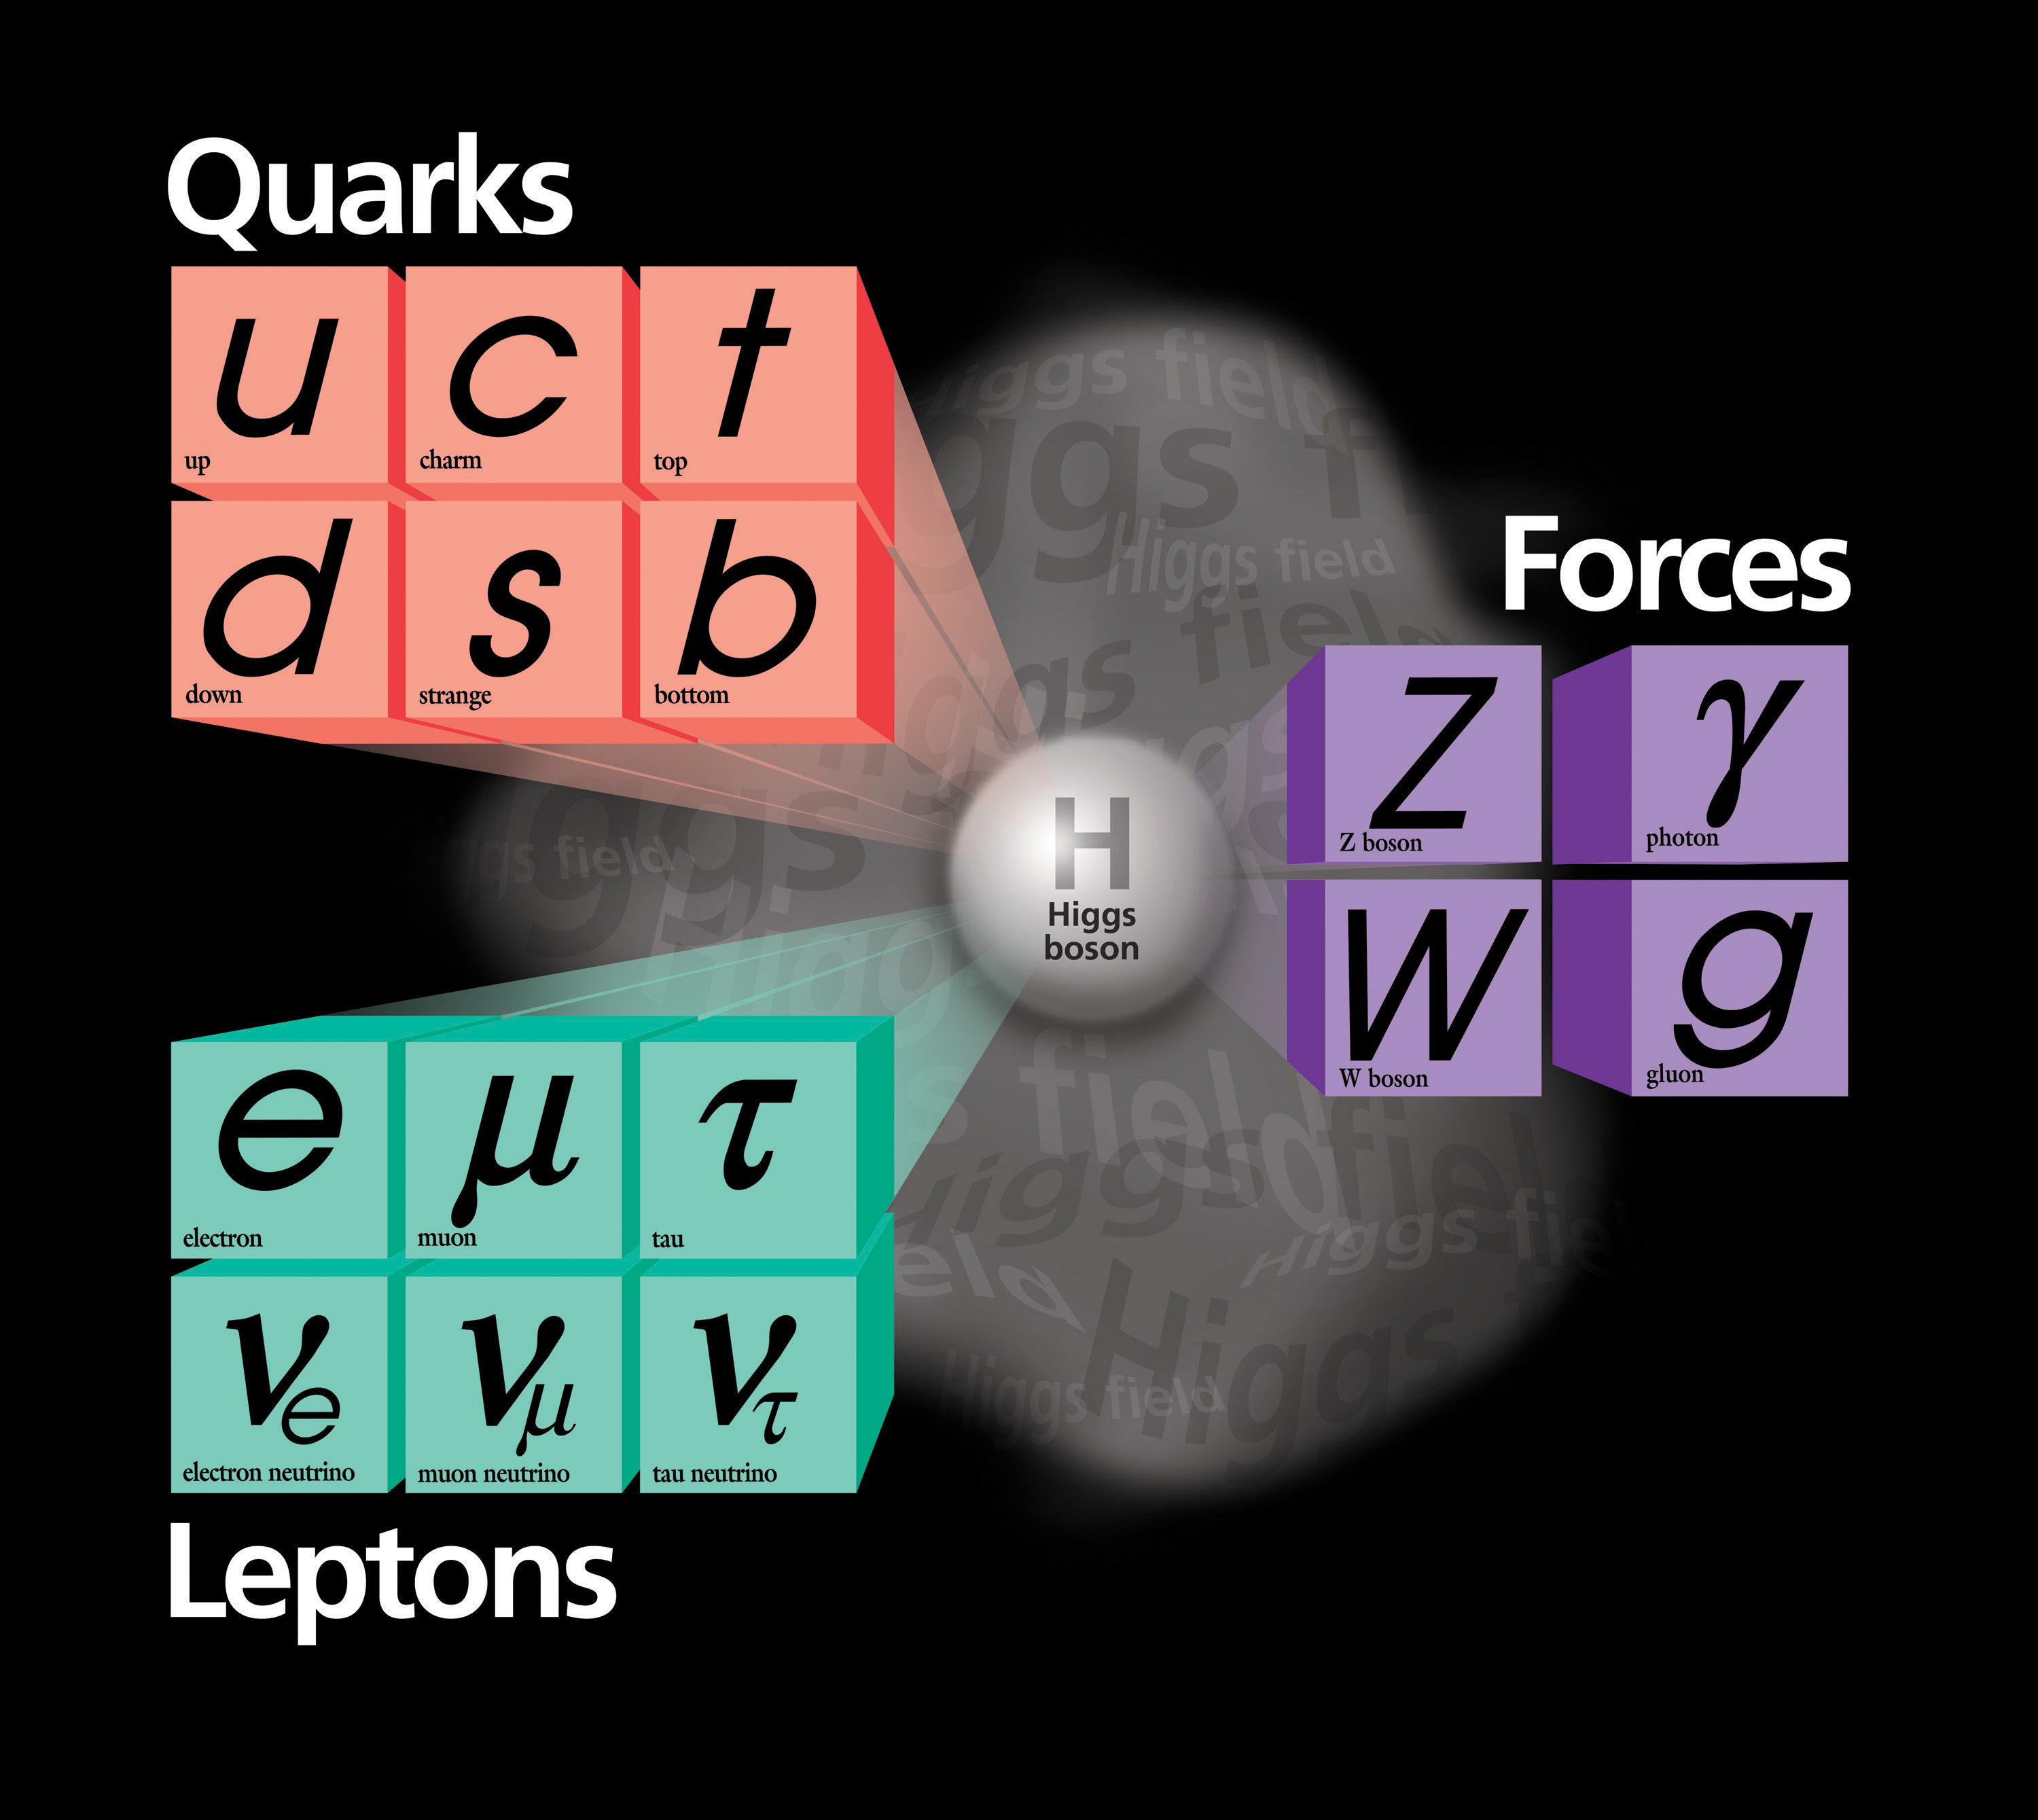
\includegraphics[width=0.6\textwidth]{plots/intro/Higgs_SM.jpeg}
\caption{Table of elementary particles: quarks and leptons (spin-1/2) are shown on the left,
the gauge bosons (spin-1) on the right, in the center the Higgs boson (spin-0).
\label{fig:parttable}}

\end{figure}

The particles within each of the weak isodoublets differ in terms of their
mass and electric charge, making them distinguishable.
 Therefore the weak isospin interaction is
 not an observed symmetry of nature, but it was clearly present
in some form given the structure of the particles table. 
In order to explain the physically observed masses and charges of elementary
 particles we need to introduce electroweak symmetry breaking, a central concept
of the SM that transforms the
weak isospin and hypercharge interactions into the well known weak and electromagnetic forces.



\subsection{The Higgs Mechanism}

What happens if a particle field takes on a non-zero expectation value in vacuum? Depending on the
quantum numbers of this non-zero field, the vacuum will not necessarily be invariant under
all symmetries of the Lagrangian. That is what is postulated by the Higgs mechanism
\cite{Anderson:1963pc,Englert:1964et,Higgs:1964pj}, where
the existence of a scalar field with non-zero vacuum expectation value
reduces the gauge symmetries of the physical 
vacuum from $\text{SU}(3)_\text{C} \times \text{SU}(2)_\text{L} \times \text{U}(1)_\text{Y}$
down to $\text{SU}(3)_\text{C} \times \text{U}(1)_\text{EM}$, thus leaving the physical vacuum invariant under
only the color and electric charges. 
The $\text{U}(1)_\text{EM}$ symmetry group requires the existence of a massless
gauge boson, the photon ($\gamma$), as the carrier of electromagnetic force.
After symmetry breaking the gauge bosons mix to form weak and electromagnetic fields:
\begin{equation}
W_{\mu}^{\pm}=\frac{1}{\sqrt{2}}\left( W_{\mu}^1 \mp W_{\mu}^{2}\right),
\end{equation}
\begin{equation}
Z_{\mu}=\cos\theta_W W_{\mu}^3-\sin\theta_W B_{\mu},
\end{equation}
\begin{equation}
A_{\mu}=\sin\theta_W W_{\mu}^3+\cos\theta_W B_{\mu}
\end{equation}
where $\theta_W$ is the weak mixing angle defined as $\theta_W=\tan^{-1} g^{'}/g$, where $g$ 
and $g^{'}$ are the coupling constants of $\text{SU}(2)_\text{L}$ and $\text{U}(1)_\text{Y}$, respectively; $A_{\mu}$ is the 
massless electromagnetic photon field ($\gamma$); and $W_{\mu}^{\pm}$ and $Z_{\mu}$ are the charged 
and neutral weak fields. The mechanism requires the introduction of a complex
scalar Higgs doublet. The potential introduced by this field breaks part of the electroweak
 gauge symmetry,
after which only one neutral Higgs scalar $H$ remains. As a result, 
the $W^{\pm}$ and $Z$ acquire masses and the photon remains massless.

\section{Open questions and physics beyond the SM}

At the current stage all the parameters of the SM have been experimentally measured,
the last being the Higgs mass, and the
self-consistency of the theory has been tested with electroweak fits \cite{Baak:2013ppa}.
%The SM is consistent with essentially all the partcile physics phenomena.
Thus far, the SM proves to be self-consistent and exhibits good agreement between
predicted and measured observables. More precise measurements and theoretical calculations
are needed in order to emphasize weak points of the SM and thus
find indirect hints of new physics.
Despite its consistency, the SM remains incomplete as it cannot answer some fundamental 
questions. I list a few of them below:
\begin{itemize}
 \item {\it the hierarchy problem} --- the gravitational interaction becomes strong only at the 
Planck scale, $10^{19}$ GeV, which is much above the electroweak scale of $\sim 100$ GeV. 
In the SM the Higgs boson mass 
depends on quantum corrections on the order of the Planck scale, unless there
exists some cancellation mechanism, such as supersymmetry \cite{Martin:1997ns}, extra dimensions
\cite{ArkaniHamed:1998rs,Zee:2003mt}, or fine-tuning; 
 \item {\it the grand unification of interactions} --- at energies of $\sim 10^{16}$ GeV
the coupling constants of the SM gauge symmetries become approximately equal, which suggests
there may exists a single gauge symmetry (typically SO(10)) with just one coupling constant
\cite{Georgi:1974sy,Buras197866};
 \item {\it the dark matter} --- it is not known how to incorporate the observed
 dark matter into the theory (should it consists of particles) \cite{Bertone2005279};
 \item {\it the neutrino masses} --- the nature of the neutrino mixing and masses is yet to be
determined as well as whether they follow Dirac or Majorana statistics \cite{Fukuda:1998fd};
 \item {\it the number of fermion generations} --- it is unknown why are there three generations
of fermions \cite{Decamp:1989tu};
 \item {\it the matter-antimatter asymmetry} --- the observable imbalance between the matter and
antimatter in the observable universe hasn't yet been explained \cite{Fukugita:1986hr};
 \item {\it the vacuum energy} --- the SM vacuum
energy density is many orders of magnitude higher when compared to astrophysical measurements
of the cosmological constant \cite{Sahni:1999gb,Rugh2002663};
\end{itemize}
Moreover, the SM involves 19 parameters, whose values are experimentally determined, but not derived from
first principles.
To overcome some of the above difficulties many theories beyond the SM have been
proposed, such as Supersymmetry (SUSY), Grand Unified Theories (GUT), extra dimensions and others.
To date none of them has been experimentally confirmed, nonetheless the searches continue.
In the next section an alternative extension of the SM known as Hidden Valleys 
is introduced. 

\section{Hidden Valleys and Long-Lived particles}

In many theories like string theory, supersymmetry, grand unification theories etc.
 one encounters large symmetry groups, which imply the existence of
new particles. In these theories the SM symmetry group $\text{SU}(3)_\text{C} \times \text{SU}(2)_\text{L} \times \text{U}(1)_\text{Y}$ 
 that we observe at the electroweak scale is only a part of a bigger picture.
The new interactions between
both ordinary and new matter will arise from the larger symmetry groups,  and  
the new states are usually
assumed to have masses around the Grand Unification or the Planck scales. However, it is not unreasonable
to assume that some of the new particles are lighter, much closer to the electroweak scale,
but there is some barrier that has thus far prevented us from finding them. A new sector
of relatively light particles not accessible because of some high energy barrier is called 
a Hidden Valley \cite{Strassler:2006im,Strassler:2006qa}.
Although, the relevant mass scale of the Hidden Valley is not well
specified, it is interesting to study scenarios that may produce visible signals within 
the reach of the LHC.
A good analogy from the SM are 
the neutrinos, which are somewhat hidden by only interacting via the massive $W$ and $Z$ bosons.
There is no reason why the new particles cannot be hidden also. 

In Hidden Valley models, the SM gauge group $G_{SM}$ is extended by a symmetry 
group of the hidden sector $G_v$. 
All SM particles carry no charges in $G_v$, while
all the new particles ($v$-particles) in the hidden sector are charged in $G_v$ and neutral 
in $G_{SM}$. Higher dimension operators (induced perhaps by a Higgs particle, a $Z^{'}$ or
a lightest supersymmetric particle) allow interaction between SM
fields and the $v$-particles.
One typically assumes that the $G_v$ is a confining, non-abelian group with the
$v$-confinement scale $\Lambda_v$, resembling the SM color group,
therefore $v$-particles assemble themselves into $G_v$-neutral $v$-hadrons.
The $v$-particles may then decay, again via higher dimension operators, to gauge invariant 
combinations of SM particles. The interactions between the SM and Hidden Valley sector are
schematically presented in Fig.~\ref{fig:hv}. 

\begin{figure}[htbp]
\centering
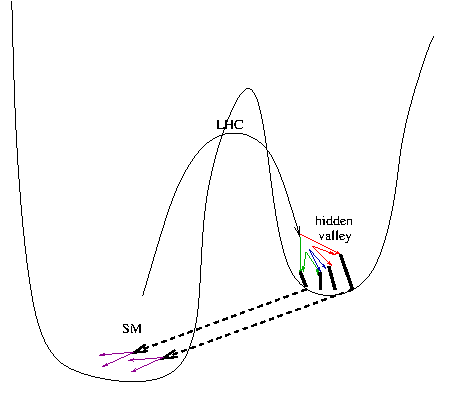
\includegraphics[width=0.6\textwidth]{plots/intro/hiddenvalley.pdf}
\caption{Schematic view of production and decay of v-hadrons. If with the energies
available at the LHC we may penetrate the barrier and produce v-hadrons, some of them may
decay back to SM particles. \label{fig:hv}}
\end{figure}

There is not a clear minimal representative for Hidden Valley models, but
many phenomena are common for a typical $v$-sector. Some examples are listed
\cite{Strassler:2006ri,Han:2007ae,Strassler:2008fv}:
\begin{itemize}
\item $v$-hadron production multiplicites at the LHC may be large, especially if $\Lambda_v\ll1$\TeV;
\item some $v$-hadrons may be stable, providing dark matter candidates and missing energy signals,
while others decay to neutral combinations of SM particles;
\item decay lifetimes can vary over many orders of magnitude, some of the $v$-particles may produce
displaced vertices;
\item some $v$-hadrons decay preferentially to heavy flavor, while others decay more democratically
to $f\bar{f}$ states ($f$ is any SM fermion), or $f\bar{f}$ plus another $v$-hadron or other final
states.
\end{itemize}

If the $v$-particles can be produced at the LHC, they can be detected via missing energy 
searches, lepton resonance searches, or displaced vertex searches. In this dissertation,
we focus on a particular signature where a long-lived $v$-particle 
decays to quark-antiquark pairs~($\qq$) at a displaced vertex,
 while we study all SM quark flavors except the top flavor. Due to the color confinement 
phenomenon, quarks
will hadronize into jets, therefore we will use the term {\it quark} and  {\it jet} as 
 equivalent from the detection perspective,
while a {\it quark-antiquark pair} will also be called a {\it dijet}.
The analysis presented in the next chapters is potentially sensitive 
to any heavy particle that decays into a pair of jets 
 at a displaced vertex. However, we study the search sensitivity and optimise the selection
 using a 
specific Hidden Valley
model as our benchmark. In this model a long-lived, spinless, neutral
exotic particle \X decays to $\qq$,
 the \X is pair-produced in the decay of a non-SM Higgs boson, i.e.  \Higgs~$\to
2$\X~, \X~$\to \qq$ \cite{Strassler:2006ri}, and 
the non-SM Higgs boson is produced through gluon-gluon
fusion. 

Several other models of new physics predict the existence of massive, 
long-lived particles which could
manifest themselves through non-prompt decays to dijets. Such scenarios arise, for example,
in various supersymmetric (SUSY) scenarios such as ``split SUSY''
\cite{Hewett:2004nw} or SUSY with very weak R-parity violation \cite{Barbier:2004ez}, 
or \Zprime models
that contain long-lived neutrinos~\cite{Basso:2008iv}. 
The outstanding feature, common in the above models,
is the existence of a massive long-lived particle that decays to {\it at least} two
quark jets. The search is therefore designed to look for pairs of hadronic jets
 that emerge from a common displaced vertex, thus allowing 
for multiple interpretations.

\section{Previous and present searches}

The CDF and D0 collaborations at the Tevatron have performed searches for metastable particles decaying to $b$-quarks
\cite{Aaltonen:2011rja, Abazov:2009ik}.
These searches are sensitive to a smaller kinematic phase space region than CMS and explore
lower masses of the exotic particles. The ATLAS collaboration
at the LHC has performed searches that are sensitive to decay lengths of 1--20\unit{m} by exploiting the ATLAS muon
 spectrometer \cite{ATLAS:2012av}, whilst the search presented here is sensitive to decay lengths 
typically below 1~m.
 The ATLAS search required the long-lived particles to be pair-produced,
while our search
is also sensitive to single or associated production.
A previous search by the CMS collaboration for long-lived particles in a similar phase-space region utilized leptonic decay channels~\cite{Chatrchyan:2012jna}.

The search presented here has been published as a CMS Physics Analysis Summary 
\cite{CMS-PAS-EXO-12-038}. Its journal publication is under way.
%An additional interpretation in terms of a SUSY model with R-parity
%violation is currently under study.

\section{Introduction}
\label{sec:Introduction}

Several models of new physics predict the existence of massive, long-lived particles which could
manifest themselves through non-prompt decays to jets. Such scenarios arise, for example,
in various supersymmetric (SUSY) scenarios such as ``split SUSY''
\cite{Hewett:2004nw} or SUSY with very weak R-parity violation \cite{Barbier:2004ez}, ``hidden valley'' models \cite{Han:2007ae}, and \Zprime models
that contain long-lived neutrinos~\cite{Basso:2008iv}.

This note presents the first search using data from the Compact Muon
Solenoid (CMS) for massive, long-lived exotic particles \X that decay 
to quark-anitquark pairs (\qq). Quarks will manifest themselves as jets of particles in the CMS detector. 
We therefore search for events
containing a pair of jets originating from a common secondary
vertex that lies within the volume of the CMS tracker and is significantly transversely displaced from the event
 primary vertex.
This topological signature has the potential to provide clear evidence for
physics beyond the standard model (SM). It is also very powerful in suppressing backgrounds from 
standard model processes.

While the analysis presented here is sensitive to any heavy particle that decays into a pair of jets
 at a displaced vertex, it is useful to have a benchmark model.
We use a specific model of a long-lived, spinless, neutral
exotic particle \X which decays to $\qq$. In this 
model, the \X is pair-produced in the decay of a non-SM Higgs boson, i.e.  \Higgs~$\to
2$\X~, \X~$\to \qq$ \cite{Strassler:2006ri}, where the Higgs boson is produced through gluon-gluon
fusion. This model predicts up to two displaced
dijet vertices within the volume of the CMS tracker per event. 

The CDF and D0 collaborations have performed searches for metastable particles decaying to b-quark jets
\cite{Aaltonen:2011rja, Abazov:2009ik}.
These searches are sensitive to a smaller kinematic phase space region than CMS and explore
lower masses of the exotic particles. The ATLAS collaboration
has performed searches that are sensitive to decay lengths of 1--20\unit{m} by exploiting the ATLAS muon
 spectrometer \cite{ATLAS:2012av}, whilst the search presented here is sensitive to decay lengths below 1 metre.
 The ATLAS search required the long-lived particles to be pair-produced,
while our search  
is also sensitive to single or associated production. 
A previous search by the CMS collaboration for long-lived particles in a similar phase-space region 
to this search utilized leptonic decay channels~\cite{Chatrchyan:2012jna}.


\chapter{The Experiment}
\label{chap:cmslhc}
\section{The Large Hadron Collider}

The Large Hadron Collider (LHC) \cite{Evans:2008zzb,Bruning:2004ej} is a colliding-beam accelerator 
of circulating beams of protons
or lead ions. 
It sits beneath the French-Swiss border outside of Geneva, in the 27-km-circumference tunnel that was originally used
for the Large Electron-Positron collider (LEP). 
 The LHC consists of two beam pipes which house counter-circulating beams.

The protons that collide in the LHC are ionized hydrogen atoms that are bunched in groups
of approximately $1.5\times10^{11}$ protons. To achieve their final energy of 4 TeV per proton,
the proton bunches undergo a series of acceleration steps before being injected into
the main LHC ring, as ilustrated in Fig. \ref{fig:accelerators}.

\begin{figure}[htbp]
\centering
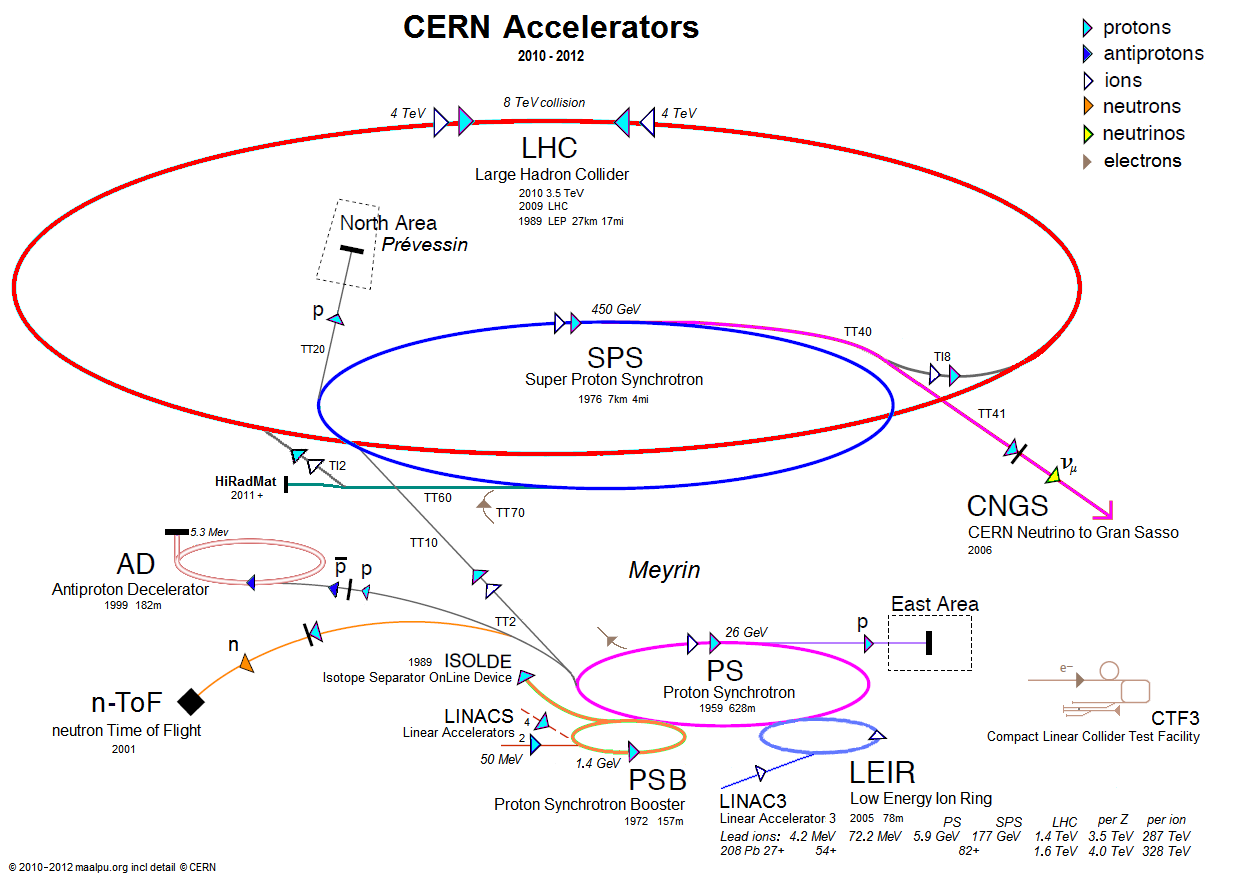
\includegraphics[width=0.9\textwidth]{plots/intro/accelerators.png}
\caption{A schematic diagram of the LHC accelerator complex.\label{fig:accelerators}}
\end{figure}

First, the protons are accelerated in the linear accelerator (LINAC) and injected into 
the Booster where they reach a kinetic energy of 1.4\GeV. The protons are then injected
in the Proton Synchrotron (PS) where the beams are arranged into bunches
with 25~ns or 50~ns spacing, and accelerated to 25\GeV. At the next step,
 proton bunches are injected
into the Super Proton Synchrotron (SPS) where they achieve energies of 450\GeV. Finally, the proton
bunches are injected into the LHC. Both LHC beams are fed from the SPS through a series of injections
until a desired number of bunches is reached in both LHC rings. Then, with accelerating 
radio-frequency cavities the beams are brought to the desired operating energies.
The center of mass collision energy for which the LHC was designed, namely 14\TeV,
 is planned to be achieved in 2015.
In 2012 the LHC operated at a reduced energy of 4\TeV per proton, for a total
center of mass energy of $\sqrt{s} = 8 \TeV$.

The beams are steered through the LHC 
using a series of 1232 superconducting dipole magnets with magnetic fields 
of up to 5.5~T for beam energy of 4\TeV. In order to provide superconductivity the 
dipoles are kept at 1.9~K using superfluid helium.
In addition to the dipoles, there are 400 quadrupole magnets used
for focusing the beams.

The LHC beams are
crossed in four sections around the ring to enable collisions of the beams. Each interaction point
houses a large detector, two general purpose ones ATLAS and CMS, and two specialized detectors
ALICE and LHCb. The ALICE and LHCb experiments took advantage of already available caverns from
the LEP experiments, while ATLAS and CMS, located at opposite sides of the LHC ring, as illustrated
in Fig. \ref{fig:lhc}, are located in caverns built specifically for them.

\begin{figure}[htbp]
\centering
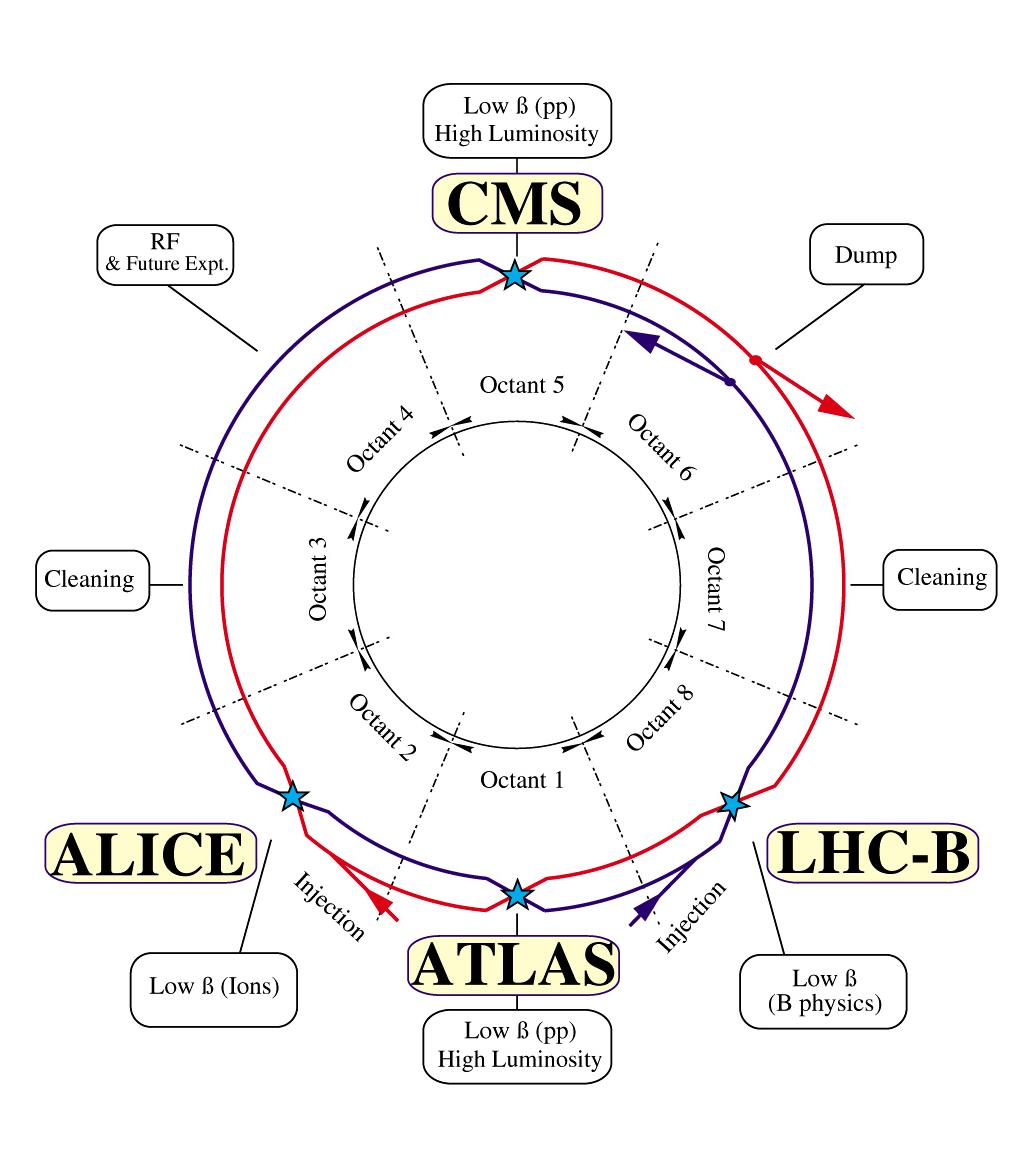
\includegraphics[width=0.6\textwidth]{plots/intro/lhc.jpg}
\caption{The layout of the LHC interaction points.\label{fig:lhc}}
\end{figure}

The instantaneous luminosity of the machine, \ie the rate of scattering events produced divided
by the cross section of the process, is given by \cite{Aaij:2011er}:
\begin{equation}
\mathcal{L}=\frac{f n_b N_p^2}{A_{\mathrm{eff}}}
\end{equation}
where $f$ is the orbit frequency ($\sim$11~kHz), $n_b$ is the number of colliding bunch pairs, 
$N_p$ is the number of protons per bunch, and $A_{\mathrm{eff}}$ is the effective 
area by which the bunches
overlap, transverse to the beam directions.


\begin{figure}[htbp]
\centering
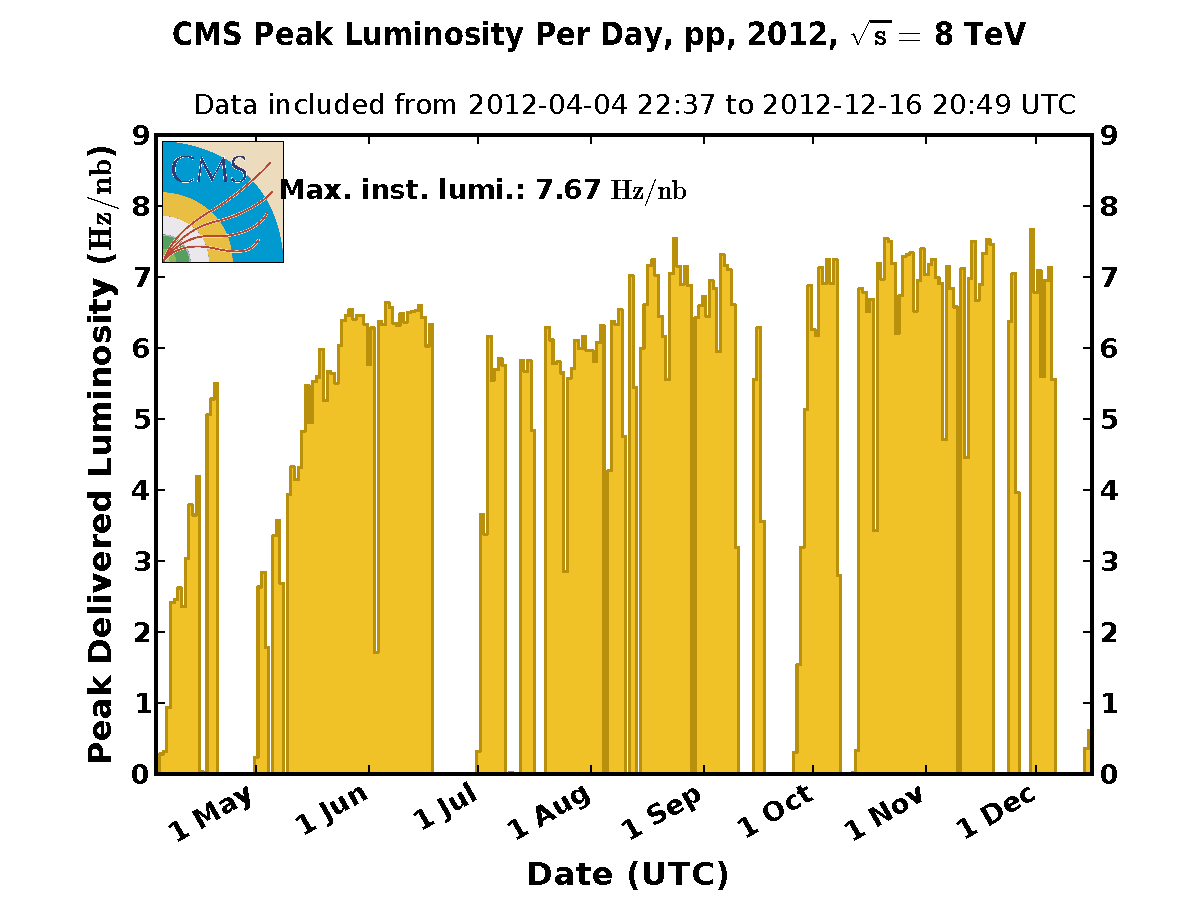
\includegraphics[width=0.49\textwidth]{plots/intro/peak_lumi.pdf}
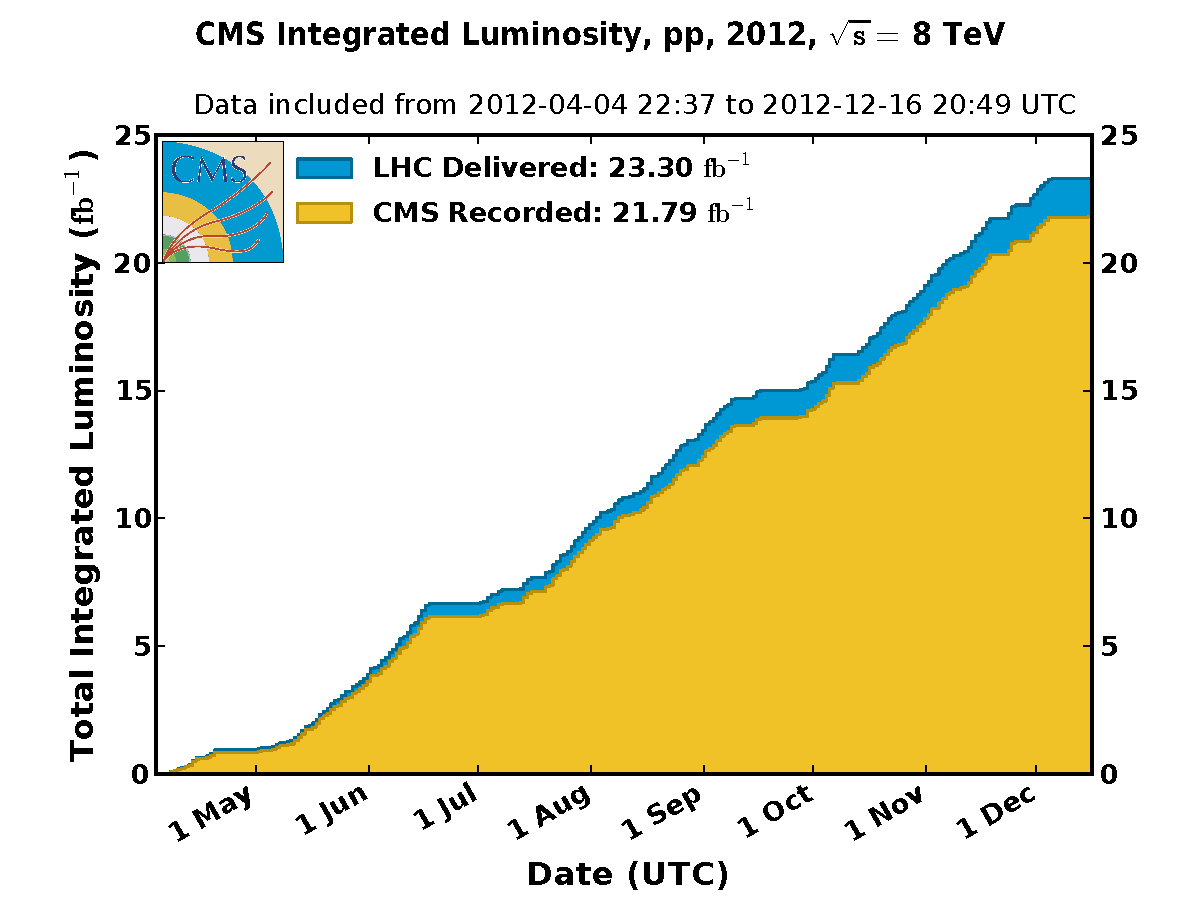
\includegraphics[width=0.49\textwidth]{plots/intro/int_lumi.pdf}
\caption{The daily peak instantaneous luminosity (left) and the integrated luminosity (right)
 delivered to the CMS experiment during the 2012 8\TeV proton-proton run.\label{fig:lumi}}
\end{figure}

The peak instantaneous luminosity per bunch during the 2012 LHC run 
 reaches 7~Hz/$\mu$b, Fig. \ref{fig:lumi}. 
Assuming a hard scattering cross section of $\sim70$~mb, there are $\sim$30 simultaneous interactions 
for each 
crossing of the proton bunches. Simultaneous presence of multiple proton-proton ($pp$) interactions
 poses a significant challenge in the form of difficult event reconstruction and analysis tasks.
 The total integrated luminosity 
delivered to the experiments in the 2012 LHC run of 23.3 \fbinv 
is the highest integrated luminosity for a hadron collider 
to date.

\section{The Compact Muon Solenoid}

The Compact Muon Solenoid (CMS) detector is designed to provide efficient identification and 
measurement of photons, electrons, muons, taus and hadronic showers over a wide range of 
transverse momentum and direction.
CMS is divided into sub-detector systems, which perform complementary roles.
The central feature of the CMS apparatus is a superconducting solenoid of 6\unit{m} internal diameter. Within the superconducting solenoid volume are a silicon pixel and strip tracker, a lead tungstate crystal electromagnetic calorimeter (ECAL), and a brass/scintillator hadron calorimeter (HCAL). Muons are measured in gas-ionization detectors embedded in the steel return yoke outside the solenoid. Extensive forward calorimetry complements the coverage provided by the barrel and endcap detectors. 
A more detailed description of the CMS detector can be found in Ref.~\cite{Chatrchyan:2008zzk}.  
The following sections describe in more detail the specific features of the CMS detector
that are crucial in the search for long-lived neutral particles decaying to jets, namely: the
tracking system, the particle-flow reconstruction and the jet reconstruction algorithm.

\subsection{Tracking system}

The tracker, the innermost detector system of the CMS detector, has a length
of 5.8 m and a
diameter of 2.5 m. It is immersed in a coaxial magnetic field of 3.8 T
provided by the CMS solenoid. A schematic drawing of the CMS tracker is shown in
Fig. 1. It comprises a silicon pixel detector with 3 barrel layers at radii
between 4.4 cm and 10.2 cm and a silicon strip tracker with 10 barrel
detection layers extending outwards to a radius of 1.1 m. Each system is
completed by endcaps which consist of 2 disks in the pixel detector and 3
plus 9 disks in the strip tracker on each side of the barrel, extending
the acceptance of the tracker up to a pseudorapidity of $|\eta| < 2.5$.
\begin{figure}[!h]
\centering
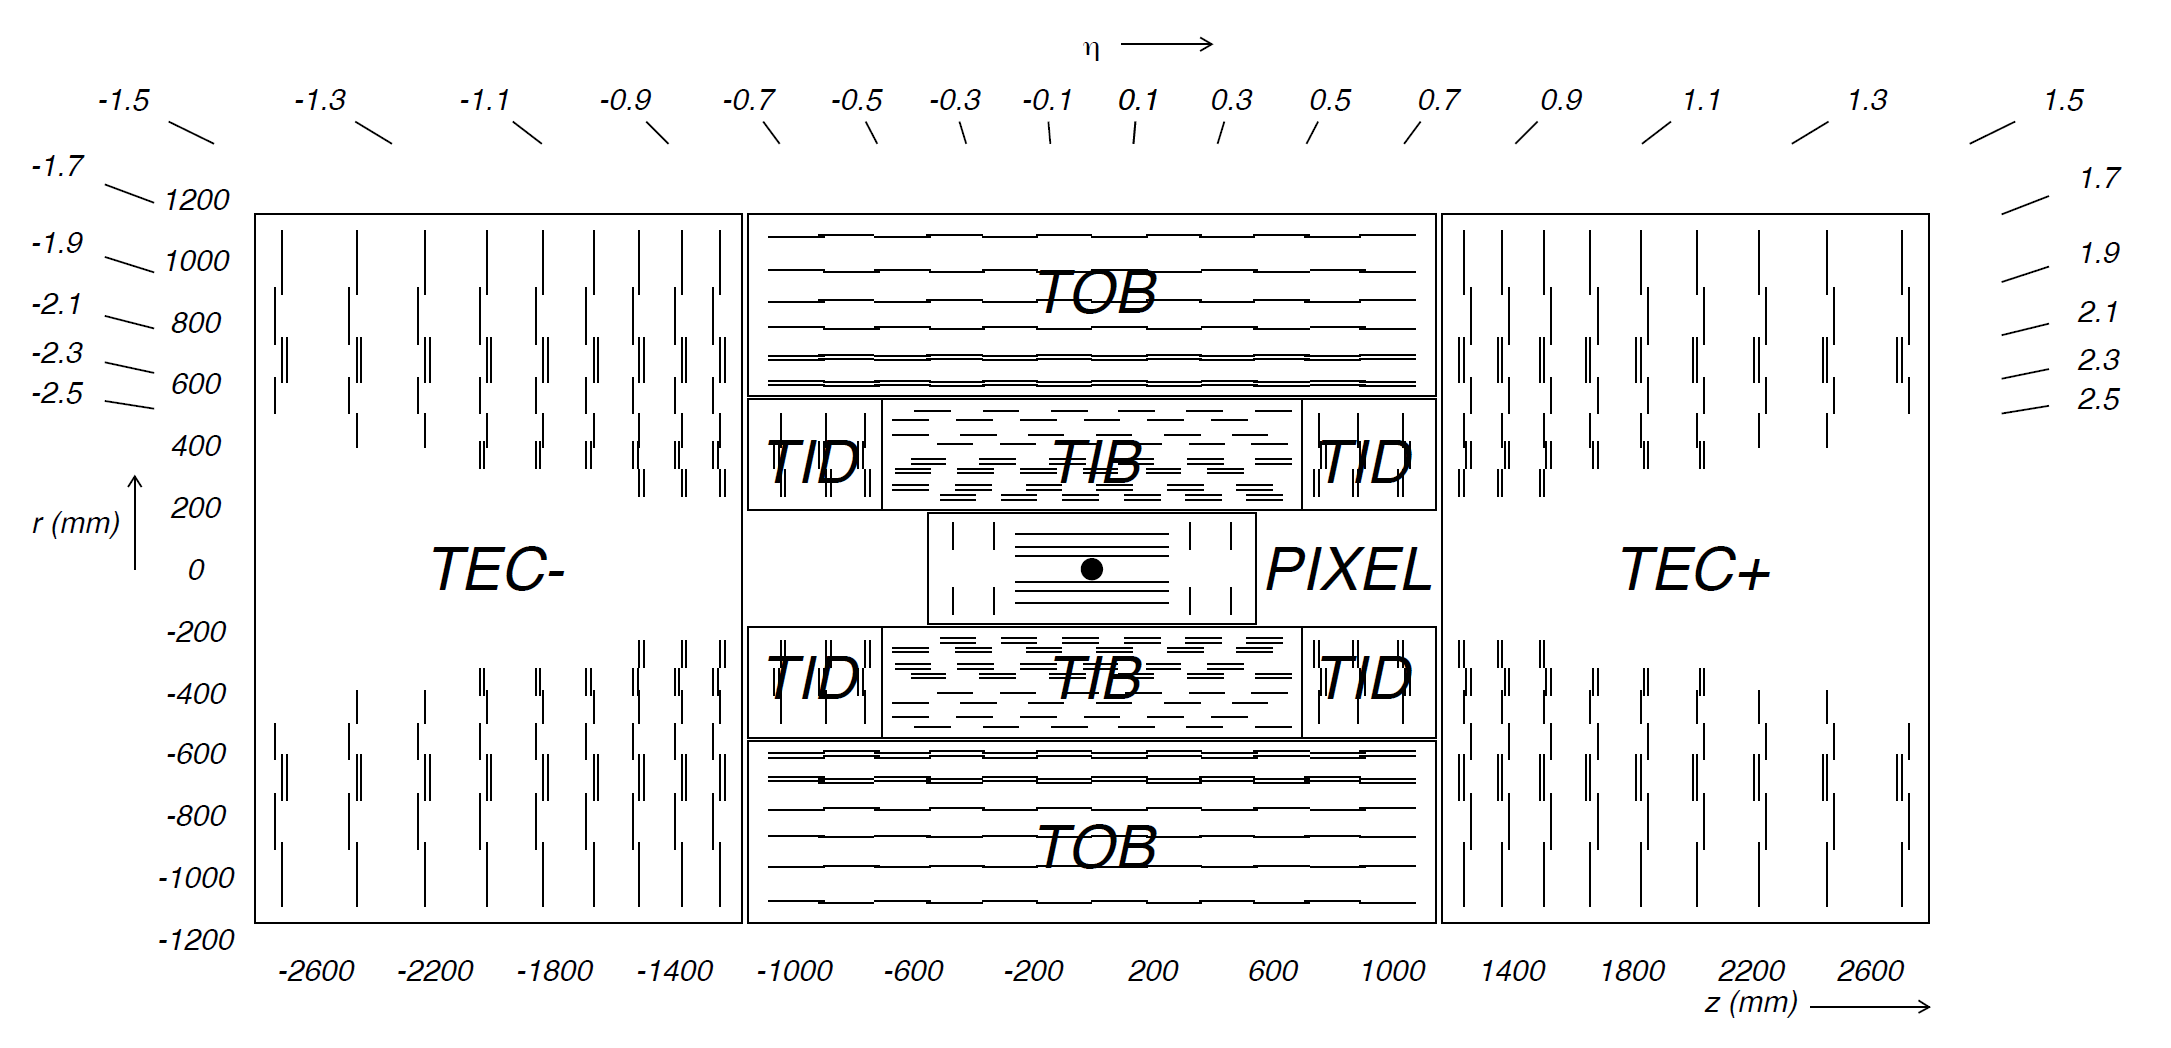
\includegraphics[width=0.99\textwidth]{plots/intro/tracker.png}
\caption{Schematic cross section through the CMS tracker. Each line represents a
detector module. Double lines indicate back-to-back modules which deliver stereo
hits.}
\end{figure}

The track reconstruction sequence is divided into 5 logical parts:
\begin{itemize}
\item \textbf{Local reconstruction} consists of clustering into \textit{hits}
the strip and pixel signals produced by charged particles on the silicon
detectors of the tracking system. The positions of the hits are estimated along
with the corresponding uncertainties;
\item \textbf{Seed generation} provides initial track-candidates for the full
track reconstruction. A seed defines initial trajectory parameters and errors;
\item \textbf{Pattern recognition} step is based on a global Kalman filter and
is responsible for finding the track-candidates that correspond to charged
particles of interest. The trajectory parameters are updated whenever a \textit{hit} is found
along the trajectory. Because the trajectories are build in parallel and allowed to share position
measurements, this part is also responsible for
cleaning the track-candidates collection by removing duplicates;
\item \textbf{Final Track fit} module estimates the final parameters of the trajectories
with ultimate precision;
\item \textbf{Track selection} rejects fake tracks by requiring that the final
tracks match a minimum set of quality criteria.
\end{itemize}

To improve the track finding efficiency, the above reconstruction procedure is
performed in six iterations. After every iteration, the hits
used for the best quality tracks (\textit{highPurity} tracks) are
locked and removed from the pool of hits available for the next iterations.
The iterations differ from each other mainly in how they
seed the tracks.
 The $0^{th}$ iteration uses pixel-triplet seeds (formed from
hits in 3 pixel layers), while the $1^{st}$ iteration uses pixel-pair seeding
(formed from hits in any 2 pixel layers), allowing it to recover tracks with
missing pixel hits due to inefficiency or acceptance. These two iterations
suffice to reconstruct the vast majority of moderately high $p_T$ tracks ($>$1GeV)
originating from the production vertex. The $2^{nd}$ and $3^{rd}$ iterations
also use pixel seeding, but since many of the Tracker hits have already been
locked by the time they run, they can use a very low $p_T$ cut or a rather
loose vertex constraint, respectively. Finally, the $4^{th}$ and $5^{th}$
iterations seed the tracks in the Strip Tracker double-layers, which provide 3D
hits by combining information from mono and stereo hits. This allows them to
find particles produced even outside the volume of the Pixel Tracker. The procedure has been optimized for using as
many tracker hits as possible while keeping the rate of fake tracks negligible.

The CMS tracker provides an impact parameter resolution of ${\sim}15\mum$ and a transverse momentum (\pt) resolution of about 1.5\% for 100\GeV particles. 
The track reconstruction algorithms are able to reconstruct displaced tracks with transverse impact
parameters up to ${\approx}30$\,cm from particles decaying up to ${\approx}60$\,cm from the beam line.  The
performance of the track reconstruction algorithms has been studied with data
\cite{Khachatryan:2010pw}. 
The silicon
tracker is also used to reconstruct the primary vertices positions with a
precision of ${\sim}20$~\mum in each dimension.

\subsection{Particle-Flow (PF) reconstruction}

The global event reconstruction (also called particle-flow event reconstruction~\cite{CMS-PAS-PFT-09-001,CMS-PAS-PFT-10-001}) is designed to reconstruct and identify each particle in the event using an optimized combination of all subdetector information.
Figure \ref{fig:cmsslice} presents schematically how various types of particles are reconstructed
with the CMS detector.

\begin{figure}[htbp]
\centering
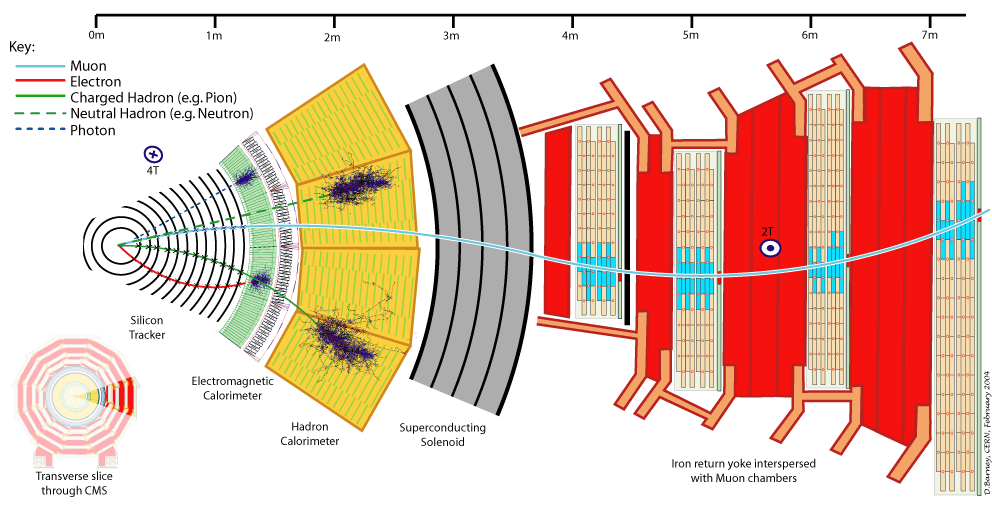
\includegraphics[width=0.99\textwidth]{plots/intro/CMS_Slice.png}
\caption{Transverse slice of the CMS detector. For each type of particle, namely muon, electron,
 photon and the neutral or charged hadron, the characteristic
signatures left in the relevant subdetectors are shown. \label{fig:cmsslice}}
\end{figure}
 
In this process, the identification of the particle type (photon, electron, muon, charged hadron, neutral hadron) plays an important role in the determination of the particle direction and energy. Photons (\eg coming from \Pgpz\ decays or from electron bremsstrahlung) are identified as ECAL energy clusters not linked to the extrapolation of any charged particle trajectory to the ECAL. Electrons (\eg coming from photon conversions in the tracker material or from \cPqb-hadron semileptonic decays) are identified as a primary charged particle track and potentially many ECAL energy clusters corresponding to this track extrapolation to the ECAL and to possible bremsstrahlung photons emitted along the way through the tracker material. Muons (\eg from \cPqb-hadron semileptonic decays) are identified as a track in the central tracker consistent with either a track or several hits in the muon system, associated with an energy deficit in the calorimeters. Charged hadrons are identified as charged particle tracks neither identified as electrons, nor as muons. Finally, neutral hadrons are identified as HCAL energy clusters not linked to any charged hadron trajectory, or as ECAL and HCAL energy excesses with respect to the expected charged hadron energy deposit. 

The energy of photons is directly obtained from the ECAL measurement, corrected for zero-suppression effects. The energy of electrons is determined from a combination of the track momentum at the main interaction vertex, the corresponding ECAL cluster energy, and the energy sum of all bremsstrahlung photons attached to the track. The energy of muons is obtained from the corresponding track momentum. The energy of charged hadrons is determined from a combination of the track momentum and the corresponding ECAL and HCAL energy, corrected for zero-suppression effects, and calibrated for the nonlinear response of the calorimeters. Finally the energy of neutral hadrons is obtained from the corresponding calibrated ECAL and HCAL energy. 

\subsection{Jet reconstruction}

For each event, hadronic jets are clustered from the particles reconstructed with the PF algorithm
 with the infrared and collinear safe
 anti-$k_\mathrm{t}$ algorithm 
operated with a size parameter $R$ of 0.5. The size parameter requires that all the jet 
particles have $\Delta R \leq 0.5$ relative to the jet momentum vector, where
 $\Delta R=\sqrt{(\Delta\phi)^2 + (\Delta\eta)^2}$ \cite{Cacciari:2008gp}. 
The jet momentum is determined as the vectorial sum of all particle momenta in this jet.
For jets originating at the event primary vertex the jet momentum is found in the simulation to be within 5\% to 10\% of the true momentum over 
the whole \pt spectrum and detector acceptance. 
When the jet origin is significantly displaced from the event primary vertex, the reduced 
charged particle efficiency results in additional underestimation of the jet momentum. 
For displaced jets originating within the volume of the CMS tracker the jet momentum is underestimated in the simulation by up to 10\%.
%Jet energy corrections are derived from the simulation, and are confirmed with in situ measurements with the energy balance of dijet and photon+jet events~\cite{CMS-PAS-JME-10-010}. The jet energy resolution amounts typically to 15\% at 10\GeV, 8\% at 100\GeV, and 4\% at 1\TeV.



\chapter{Event Selection}
\label{chap:selection}
\section{Datasets and Triggers}
\label{sec:samples}
For this analysis, pp collision data at a centre-of-mass energy of 8~TeV corresponding to an integrated
luminosity of $18.6 \pm 0.8$ ~\fbinv delivered by the LHC in 2012 are used. 
Data have been collected with dedicated displaced jet triggers. Displaced jet triggers require
the transverse energy sum
of all jets, $H_T$, to be above 300 \GeV and further demand the presence of one or two jets with $p_T>$60\GeV,
each having not more than 2 associated tracks with impact parameters below 300\mum. Additionally, the energy 
contribution of associated tracks with transverse impact parameters below 500\mum is required to be less than
15\% of the total jet energy. Impact parameters are computed with respect to the leading primary vertex 
in the event.
%A detailed description of the displaced jet triggers together with
%the trigger efficiency for all signal Monte Carlo samples listed in Table \ref{tab:signalMC} 
%can be found in \cite{CMS_AN_2011-488}. 
Data collected by the double displaced jet trigger, where presence of two triggering jets is required,
 is used to search for our signal, 
while data collected by the single jet one, where presence of only one triggering jet is required, is used
as a control sample. The integrated luminosity and the number of events collected by CMS with the
displaced jet triggers during the 2012 LHC run are summarized in Table
\ref{tab:triggerEvents}.   

\begin{table}[hbtp]
\begin{center}
\begin{tabular}{l c c c }
\hline
trigger name & prescale factor & \lumi [\fbinv] & N events [1e6] \\
\hline 
HLT\_HT300\_SingleDisplacedPFJet60 & 100-120 & 0.18 & 0.5\\
HLT\_HT300\_DoubleDisplacedPFJet60 & 1 & 18.6 & 1.9\\
\hline
\end{tabular}
\end{center}
\caption{Displaced jet triggers active in 2012 LHC run.\label{tab:triggerEvents}}
\end{table}

Signal Monte Carlo (MC) simulation samples are generated using \PYTHIA V6.424 \cite{PYTHIA} to
simulate \Higgs~production through gluon fusion ($gg \to \Higgs$). Using \PYTHIA PYUPDA cards,
subsequently the \Higgs~is forced to decay to two long-lived, spin~0, exotic particles
($\Higgs \to 2\X$), which each then decays to quark-antiquark pairs ($\X \to \qq$).
The long-lived exotic \X decays to any flavor \qq pair, excluding \ttbar, with equal probability. Samples
with different combinations of \Higgs~masses ($M_{\Higgs}$ = 120, 200, 400, 1000 \GeV ) and \X~boson masses
($M_{\X}$ = 20, 50, 150, 350 \GeV) are generated. These are listed in Table~\ref{tab:signalMC}. The
\X boson ~lifetime used in these samples is chosen to give a mean transverse decay length of approximately
2\cm, 20\cm and 200\cm in the laboratory frame. Such a selection of laboratory frame lifetimes is chosen in 
order to maximally explore the capabilities of the CMS detector for reconstructing long-lived particles.
The distributions of the \Higgs $p_T$ and resulting \X $p_T$ and $\eta$ spectra for selected signal
models are presented in Figure \ref{fig:sigHX}.

\begin{figure}[htbp]
\centering
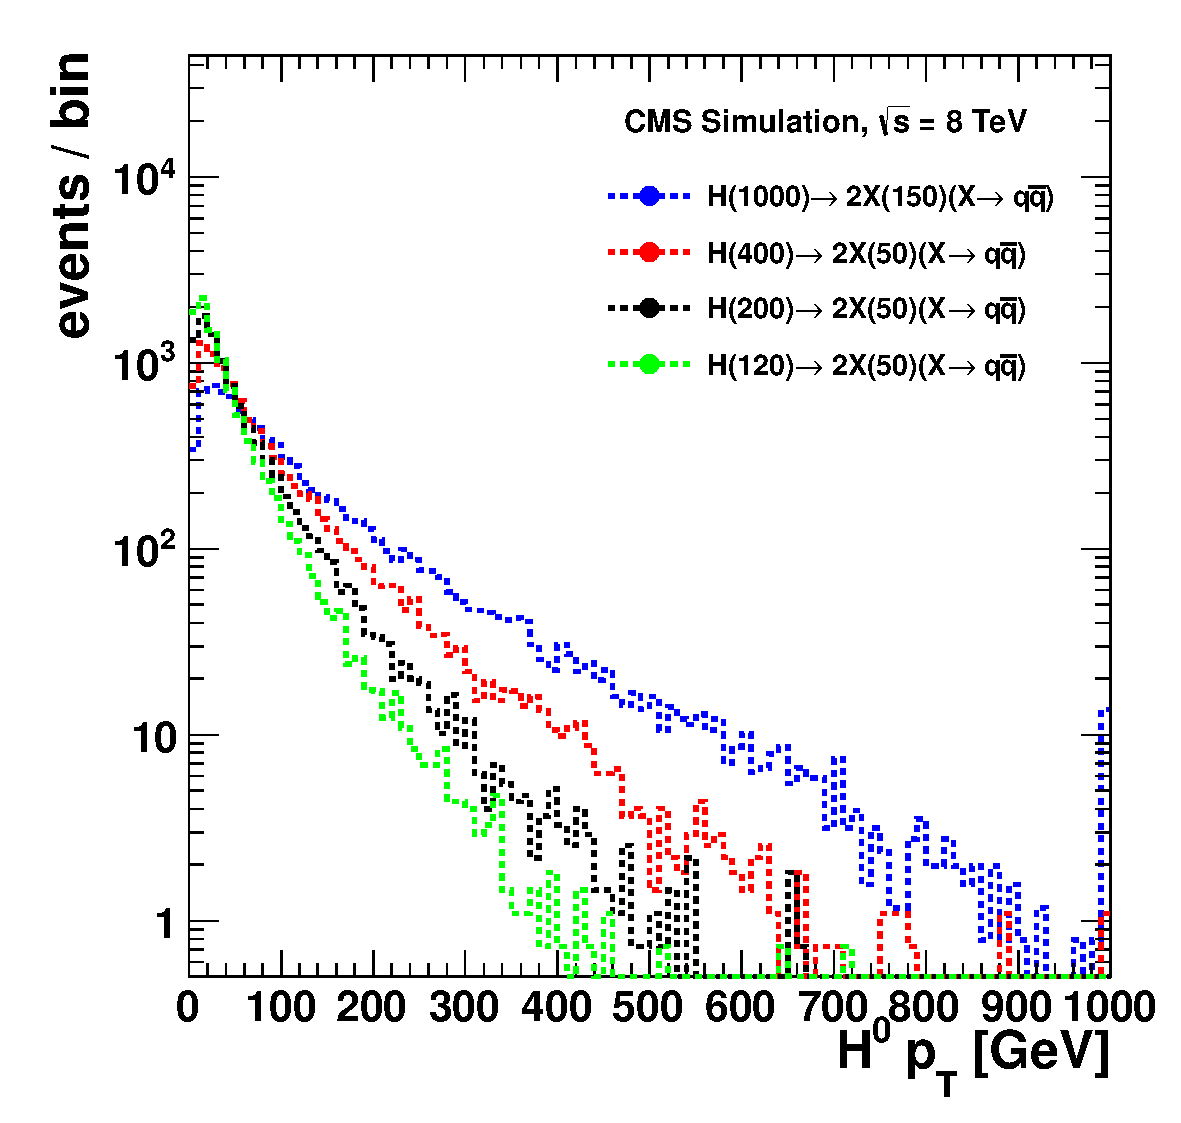
\includegraphics[width=0.495\textwidth]{plots/signal/hpt.pdf}
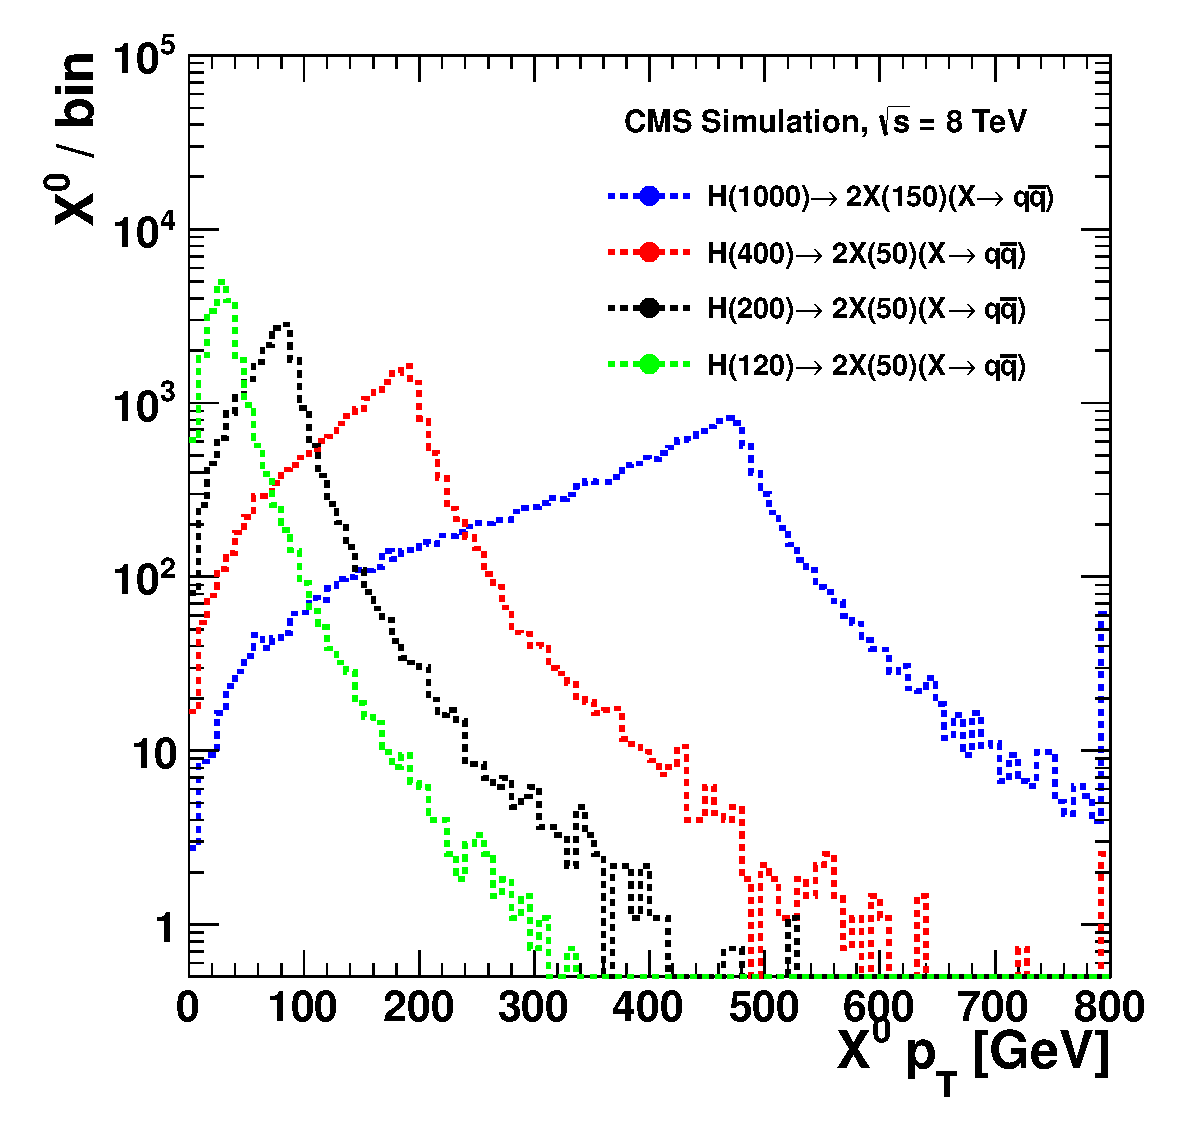
\includegraphics[width=0.495\textwidth]{plots/signal/xpt.pdf}
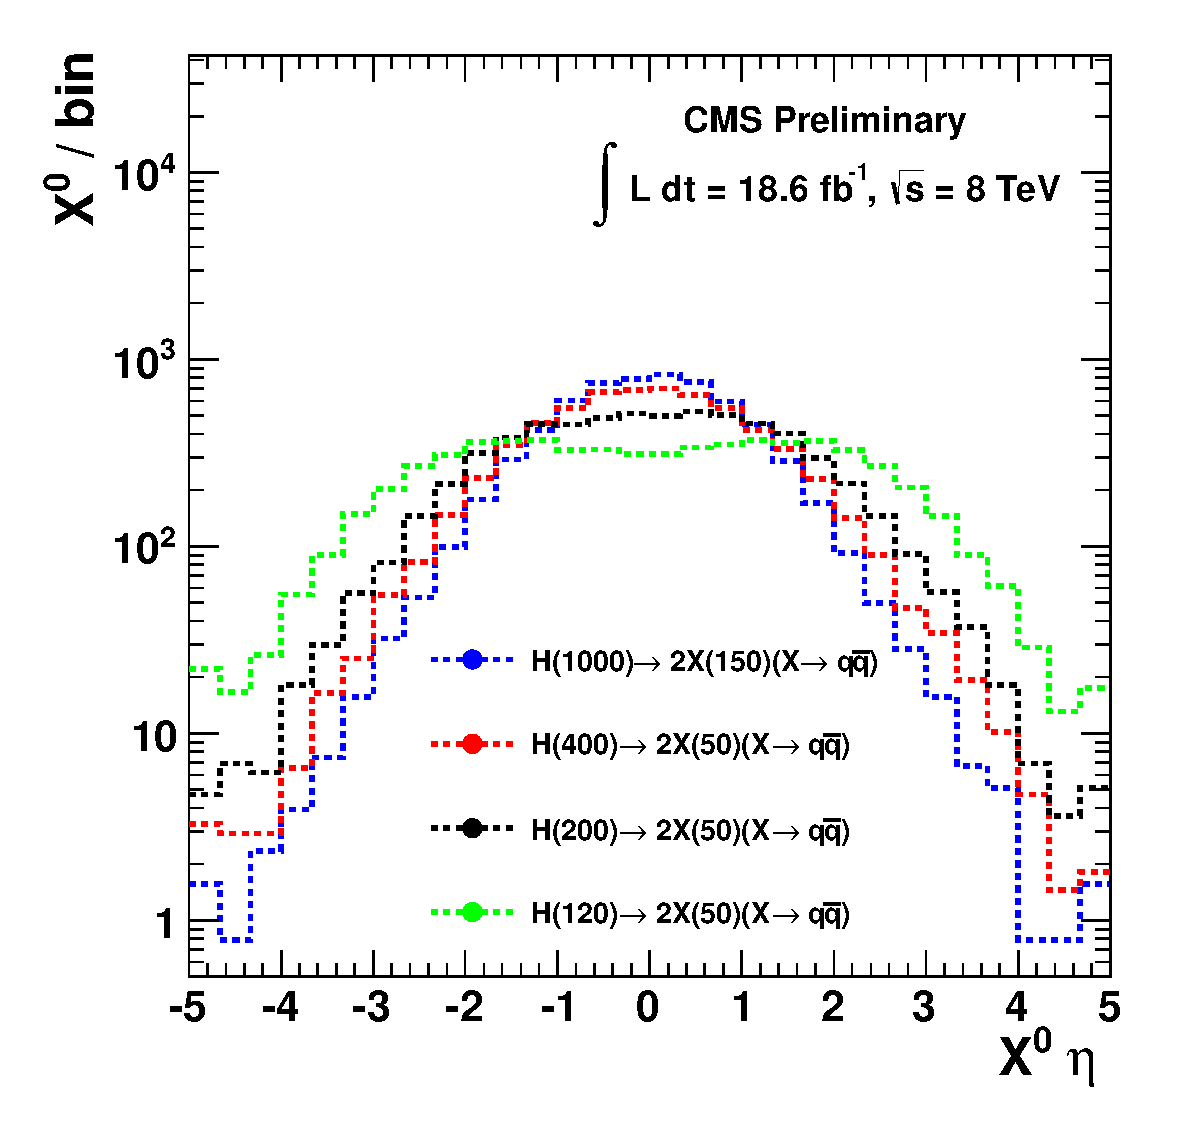
\includegraphics[width=0.495\textwidth]{plots/signal/xeta.pdf}
\caption{Generated \Higgs $p_T$ and \X $p_T$ and $\eta$ distributions for selected signal models.\label{fig:sigHX}}
\end{figure} 

The only significant background is expected to arise from QCD events, and the corresponding simulated samples
are listed in Table~\ref{tab:backgrMC}.
For each simulated background sample the number of events passing the signal trigger
scaled to the total integrated luminosity is shown. The per event weight factors that are applied according to the
number of events available in each sample are also given. The weight factors for samples with $\hat{p_T}$ 
below 470\GeV are significantly above 1, therefore the amount of simulated events in this region is insufficient. 
The background contribution   
significantly decreases with increased $\hat{p_T}$, therefore we do not consider samples with $\hat{p_T}$ higher
than 800 \GeV. For QCD events with $\hat{p_T}$ below 80\GeV the small efficiency of passing the trigger
 requirement of $H_T>$300\GeV 
makes the low $\hat{p_T}$ contribution negligible.  
In all the samples, the response of the detector is simulated
in detail using \GEANTfour~\cite{GEANT4}. The samples are then processed through the trigger emulation and
event reconstruction chain of the CMS experiment. An example event display of a reconstructed 
simulated signal event is presented in Figure \ref{fig:eventDisplay}.

\begin{figure}[htbp]
\centering
 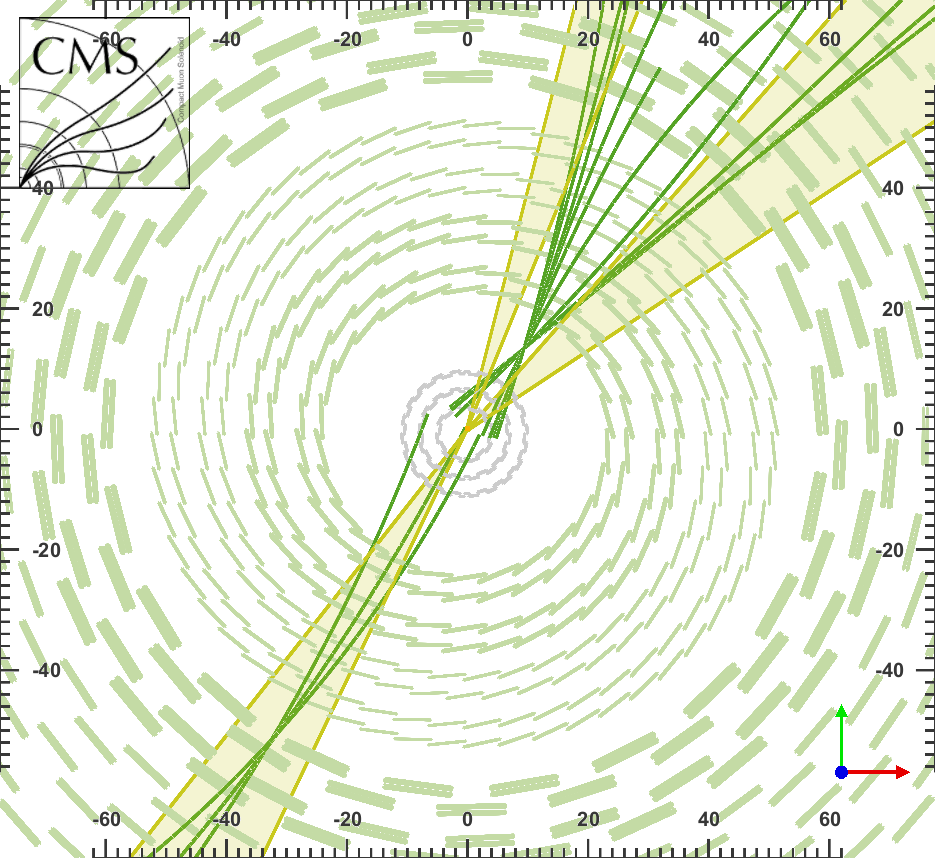
\includegraphics[width=0.6\textwidth]{plots/eventDisplay.png}
\caption{CMS event display of an example simulated signal event with a di-jet pair originating from a transversly displaced secondary vertex. \label{fig:eventDisplay}}
\end{figure}
 
\begin{table}[hbtp]
\begin{center}
\caption{Simulated signal samples used in the analysis. The masses of the \Higgs and \X bosons are given, 
as is the mean proper decay length of the \X~boson. \label{tab:signalMC}}
\begin{tabular}{|c|c|c|}
\hline 
  $M_{\Higgs}$ (\GeV) & $M_{\X}$ (\GeV) & $c\tau$ (cm) \\
\hline
       1000      &       350      &     3.5, 35, 350      \\          
       1000      &       150      &     1, 10, 100      \\          
       1000      &        50      &     0.4, 4, 40      \\          
       1000      &        20      &     0.15, 1.5, 15       \\          
       ~400      &       150      &     4, 40, 400      \\          
       ~400      &        50      &     0.8, 8, 80      \\          
       ~400      &        20      &     0.4, 4, 40      \\          
       ~200      &        50      &     2, 20, 200      \\          
       ~200      &        20      &     0.7, 7, 70      \\          
       ~120      &        50      &     5, 50, 500      \\          
       ~120      &        20      &     1.3, 13, 130      \\          
\hline
\end{tabular}
\end{center}
\end{table}


\begin{table}[hbtp]
\begin{center}
\caption{Simulated background samples used in the analysis.\label{tab:backgrMC}}.
\begin{tabular}{|l|c|c|c|}
\hline 
 \multicolumn{1}{|c|}{Dataset name} & Cross section  & Number of events passing  & Per event \\
                                    &     (pb)       & the trigger / 18.6 \fbinv & weight factor \\ 
\hline
\texttt{\small QCD\_Pt-600to800\_TuneZ2\_8TeV\_pythia6}               & 2.70e1       & 4.5e2 & 0.1  \\
\texttt{\small QCD\_Pt-470to600\_TuneZ2\_8TeV\_pythia6}               & 1.14e2       & 1.7e3 & 0.6 \\
\texttt{\small QCD\_Pt-300to470\_TuneZ2\_8TeV\_pythia6}               & 1.76e3        & 2.6e4 & 5.5 \\
\texttt{\small QCD\_Pt-170to300\_TuneZ2\_8TeV\_pythia6}               & 3.41e4 & 5.2e5 & 1.1e2 \\
\texttt{\small QCD\_Pt-120to170\_TuneZ2\_8TeV\_pythia6}               & 1.56e5  & 7.5e5 & 4.8e2 \\
\texttt{\small QCD\_Pt-80to120\_TuneZ2\_8TeV\_pythia6}                & 1.03e6  & 4.8e5 & 3.2e3 \\
\texttt{\small QCD\_Pt-50to80\_TuneZ2\_8TeV\_pythia6}                & 8.15e6  & 1.1e5 & 2.5e4 \\
\hline
\end{tabular}
\end{center}
\end{table}

 
\section{Event Reconstruction and Selection}

\subsection{Signal model sensitivity}
\label{subsec:sigsensitivity}

\subsubsection{\Higgs mass}

The \Higgs mass range sensitivity is mostly affected by the $H_T>300\GeV$ requirement imposed by the trigger. 
In order to provide trigger efficiency to this trigger filter,
we require $H_T>325\GeV$ in the offline reconstruction.

\begin{figure}[htbp]
\centering
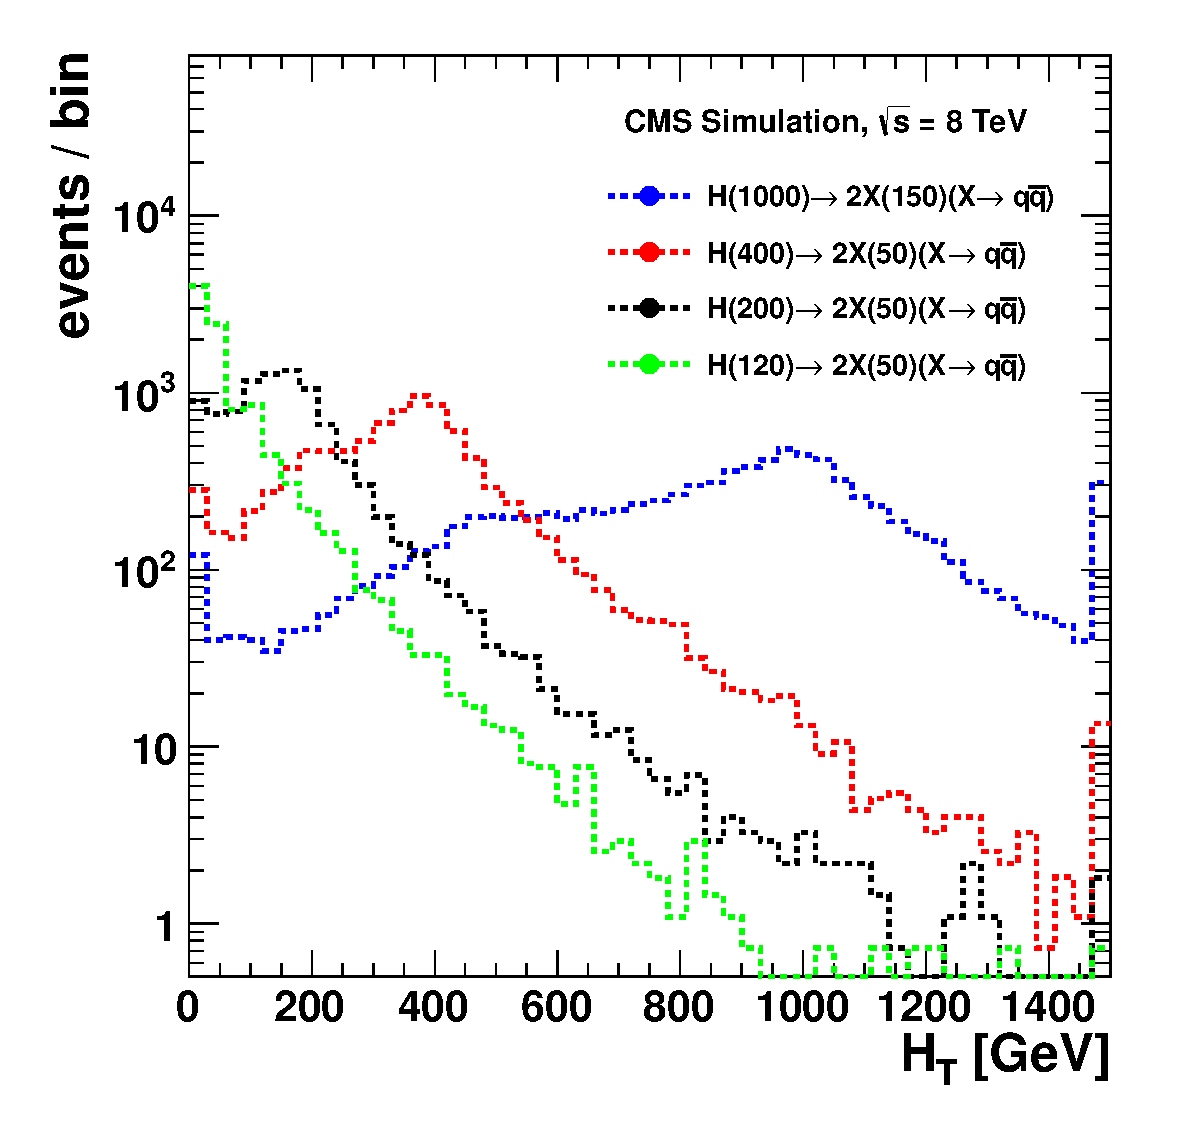
\includegraphics[width=0.49\textwidth]{plots/signal/ht.pdf}
\caption{$H_T$ distributions for the benchmark signal models.\label{fig:sight}}
\end{figure}

Figure \ref{fig:sight} presents the $H_T$ distributions for selected signal models; all available \Higgs 
mass points are shown.
The $H_T>325\GeV$ requirement reduces the sensitivity of the search in the low mass region of the exotic \Higgs,
therefore we analyze further only those signal models where mass of the \Higgs is 200\GeV or higher.

\subsubsection{\X mass given the \Higgs mass}

In this analysis we aim to reconstruct displaced dijet candidates originating from a common displaced
vertex using pairs of 
Particle Flow (PF) jets \cite{CMS-PAS-PFT-09-001} within the tracker acceptance ($|\eta|<2$).  
 PF jets are reconstructed with an anti-k$_T$
algorithm operated with a size parameter $R$ of 0.5 \cite{Cacciari:2008gp} which determines
the minimal angular distance between the jets. In order to reconstruct two distinct
jets with this algorithm the opening angle between the two quarks needs to be above 0.5 radians.
Figure \ref{fig:sigdR} presents the opening angle distributions between the two quarks originating
from $\X \to \qq $ decay for signal models with 
$M_{\Higgs}$=200,400,1000 \GeV.  

\begin{figure}[htbp]
\centering
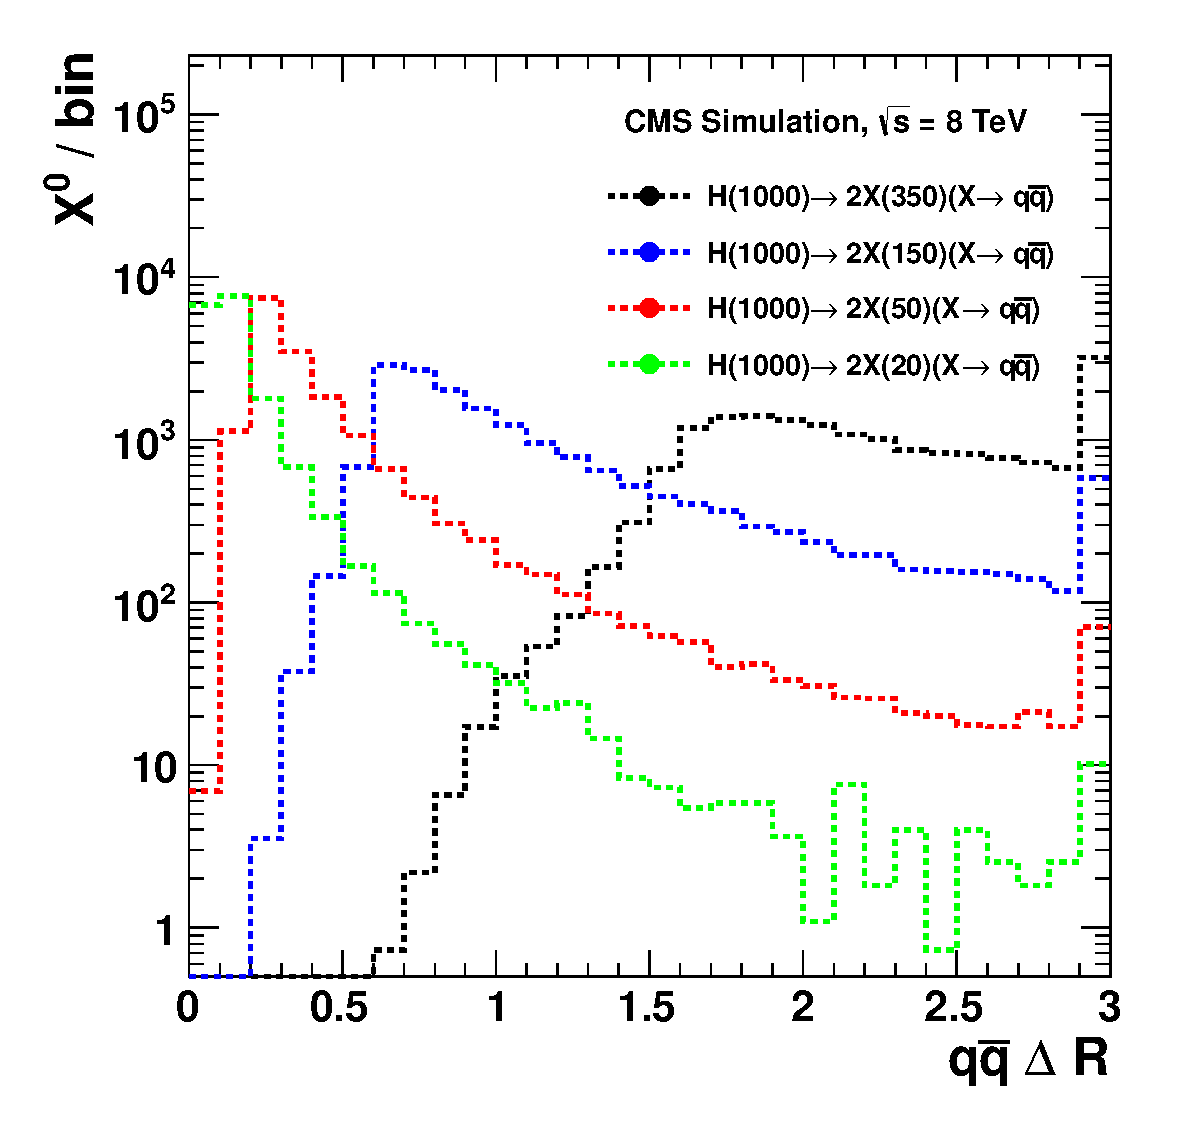
\includegraphics[width=0.49\textwidth]{plots/signal/dRH1000.pdf}
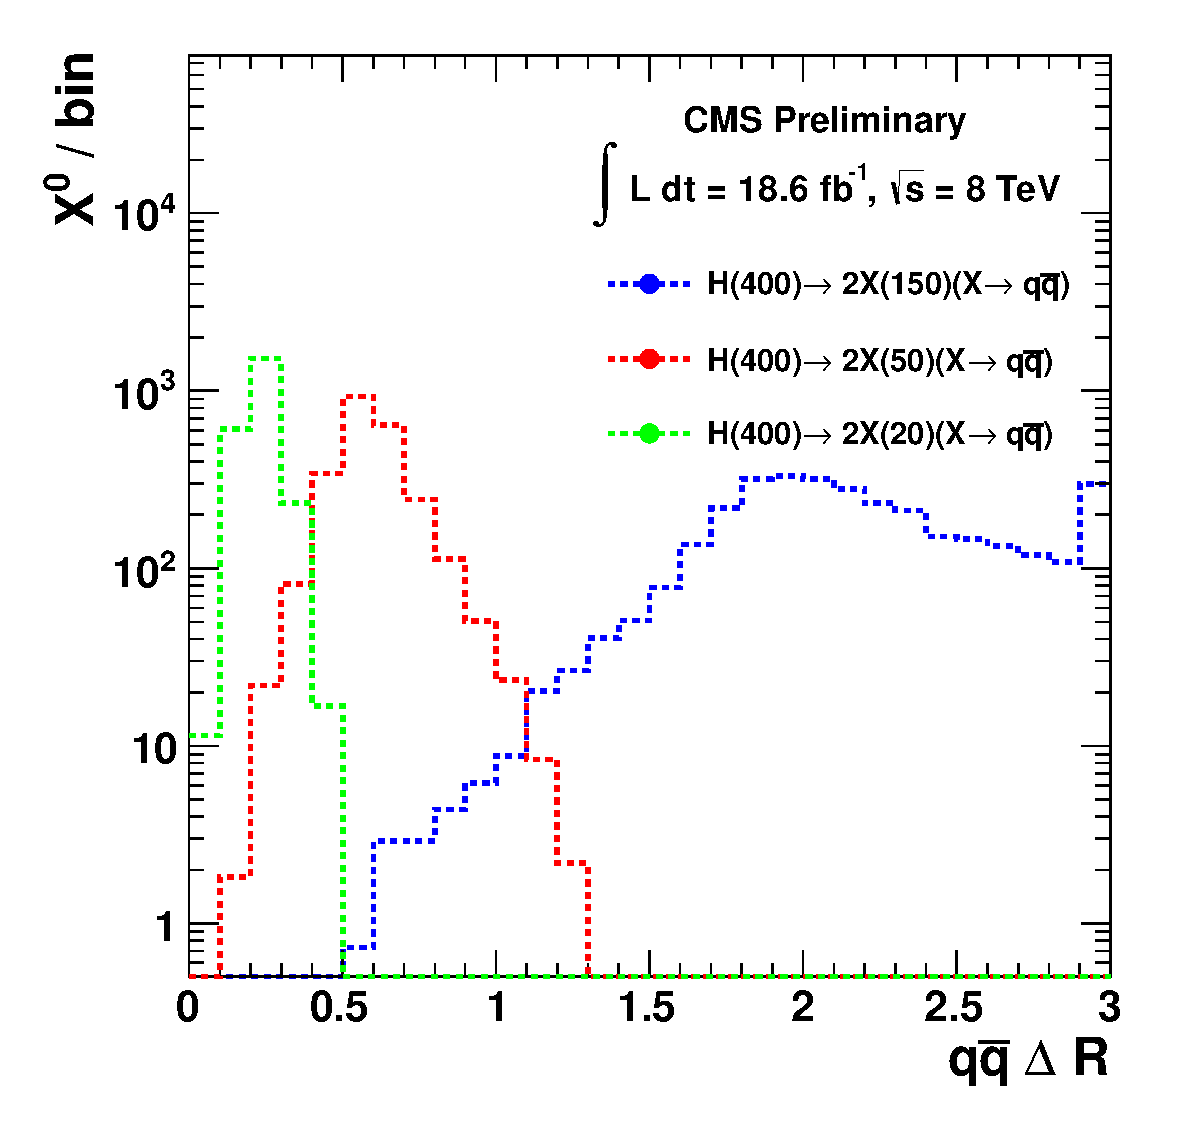
\includegraphics[width=0.49\textwidth]{plots/signal/dRH400.pdf}
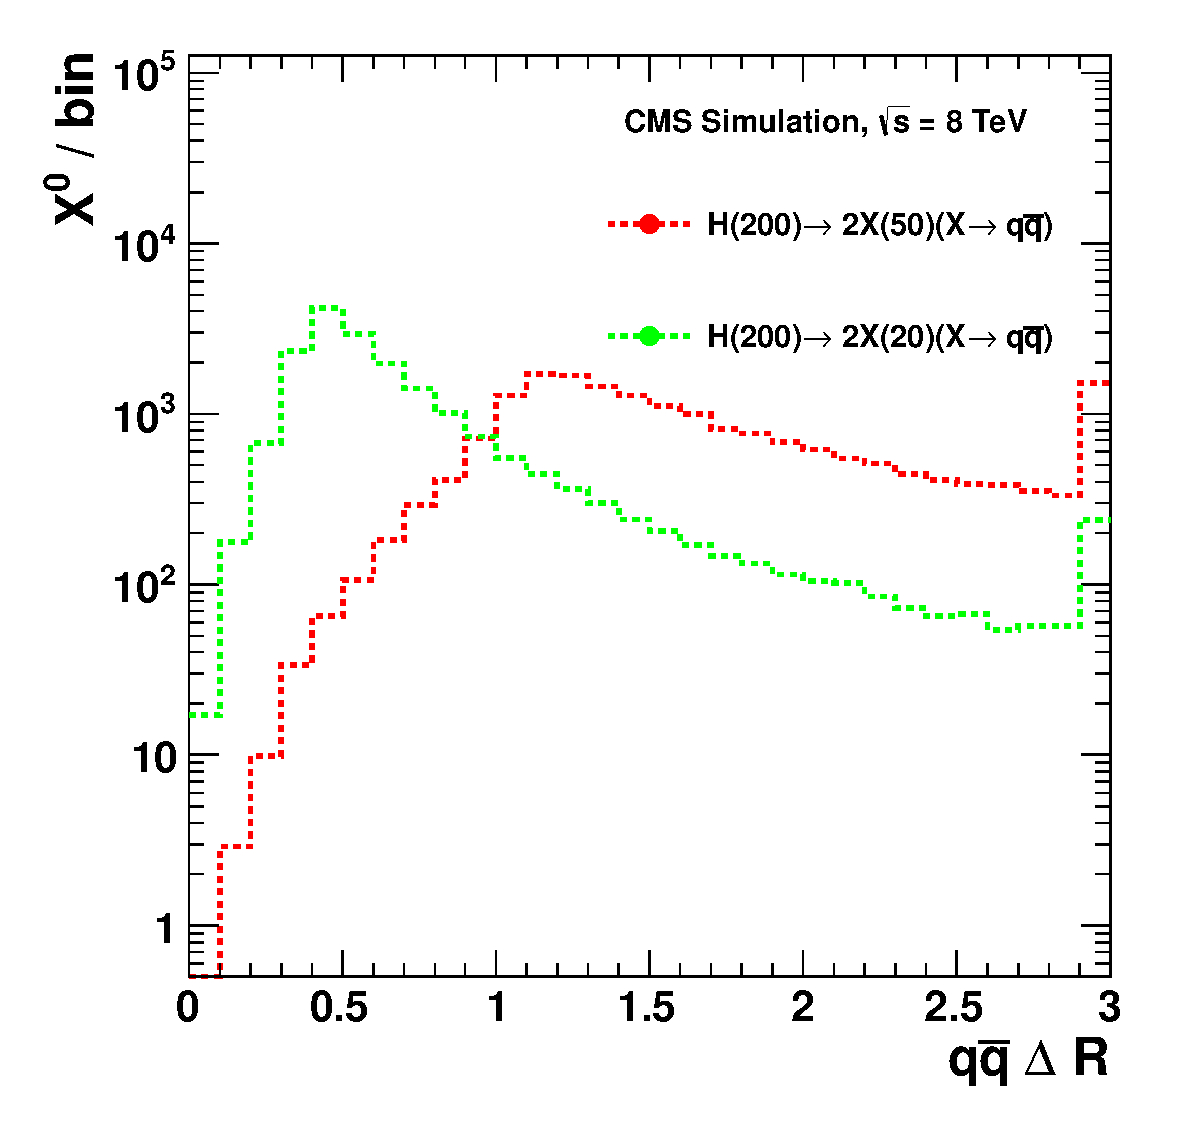
\includegraphics[width=0.49\textwidth]{plots/signal/dRH200.pdf}
\caption{Opening angle distributions of the $\qq$ pair originating from the $\X \to \qq$ decay as a function
of \Higgs and \X particles masses. \label{fig:sigdR}}
\end{figure}

\begin{figure}[htbp]
\centering
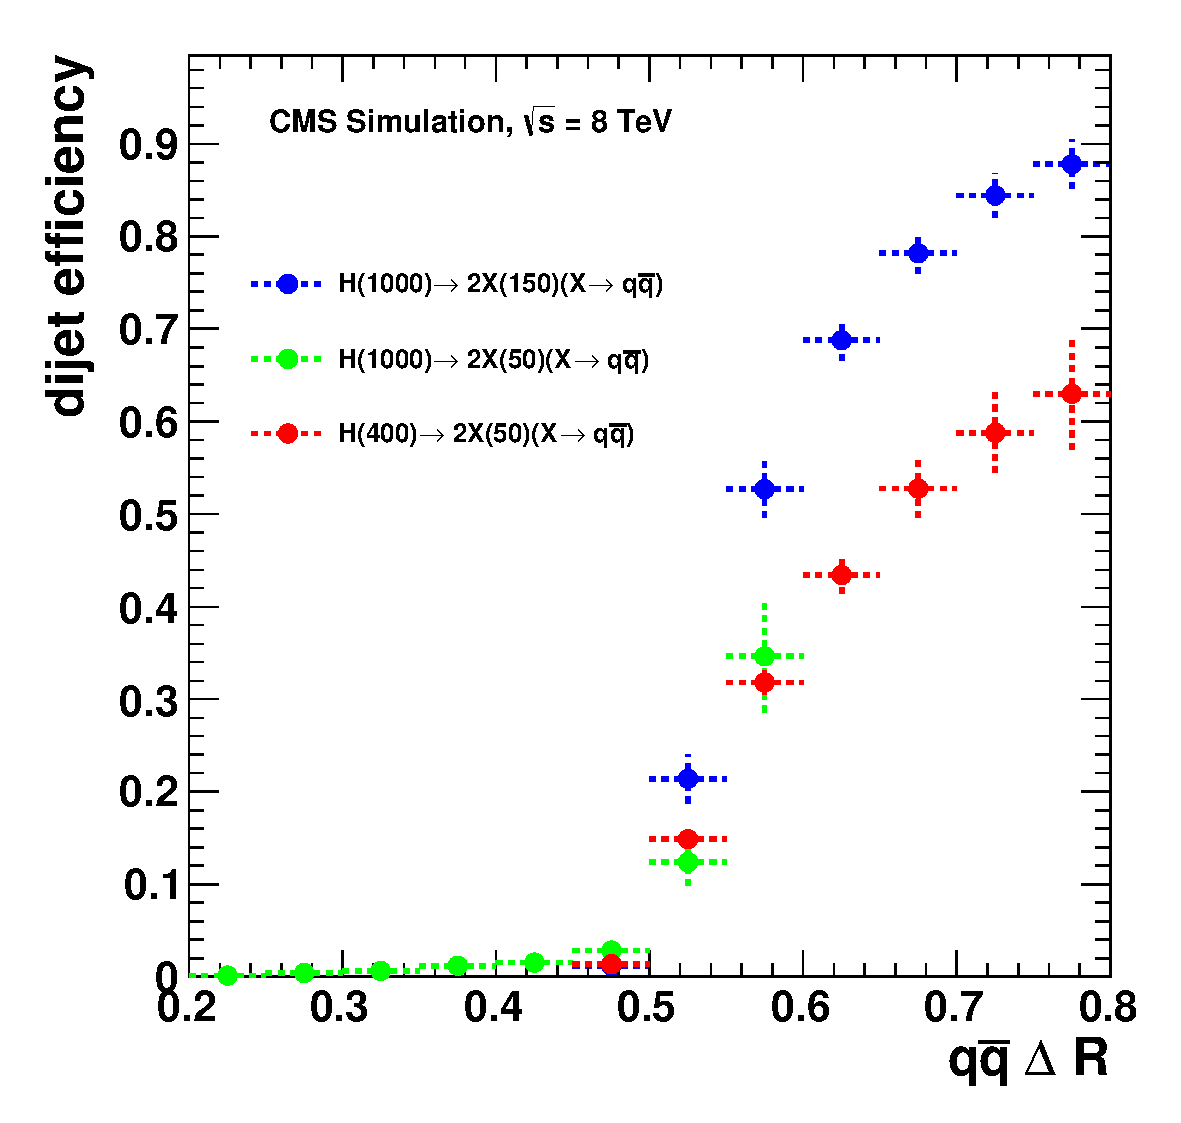
\includegraphics[width=0.49\textwidth]{plots/signal/effDijet.pdf}
\caption{Dijet reconstruction efficiency as a function of the quarks opening angle for jets reconstructed with an
anti-k$_T$ algorithm operated with a cone size of 0.5. Both reconstructed jets are required to have a $p_T>60$\GeV
and $|\eta|<2$.  \label{fig:effdR}}
\end{figure}

The efficiency of reconstructing a pair of jets
 corresponding to the $\X \to \qq$ decay using anti-k$_T$ algorithm with the 0.5 radius as a function of the
opening angle of the quark pair is shown in Figure \ref{fig:effdR}. Both jets are required 
to have the $p_T>60$\GeV and $|\eta|<2$ which causes the 
efficiency to be reduced for lower \Higgs  mass models.
 

The dijet analysis is therefore sensitive to the mass points of the long-lived particles \X for which 
a significant fraction of candidates have the quarks opening angle above 0.5, namely:
\begin{itemize}
\item $M_{\X}$ between 150-350\GeV for $M_{\Higgs}$=1000\GeV
\item $M_{\X}$ between 50-150\GeV for $M_{\Higgs}$=400\GeV
\item $M_{\X}$=50\GeV for $M_{\Higgs}$=200\GeV
\end{itemize}

Given the kinematic constraints we define the following acceptance criteria 
for the \X candidates at the generator level:
\begin{itemize}
 \item $\qq$ opening angle above 0.5;
 \item $p_T>40\GeV$ and $|\eta|<2.1$ for both quarks from the $\X \to \qq$ decay;
 \item transverse decay length, $L_{xy}<60\cm$ - the CMS tracker allows for track reconstruction originating at
a transverse displacement up to 60\cm, therefore secondary vertices with higher displacement cannot be reconstructed.
\end{itemize}

%All reconstructed signal dijet candidates that pass full selection criteria fulfill the acceptance definition. 

\subsection{Event filters}

The following event filters are applied to mitigate known detector effects affecting the quality of the data
acquired by CMS during the 2012 LHC run:
\begin{itemize}
\item {\bf primary vertex filter} - events are required to contain a primary vertex with at least four associated
tracks whose position is displaced from the nominal interaction point by no more than 2 \cm in the direction
transverse to the beam and no more than 24 \cm in the direction along the beam;
\item {\bf beam background filter} - each event is required to contain at least 10 tracks with at least 25\% of them 
being high-purity tracks;
\item {\bf beam halo filter} - events containing beam halo muons are rejected;
\item {\bf HBHE noise filter} - events with anomalous noise activity in the HCAL electronics readout are filtered;
\item {\bf HCAL laser event filter} - events with a spurious trigger of the HCAL calibration laser are removed;
\item {\bf anomalous ECAL super-crystal energy filter} - concerns a handful of super-crystals in the ECAL endcap region
which occasionally give anomalously high energies;
\item {\bf ECAL laser correction filter} - events are rejected when ECAL crystals are assigned very high transparency
corrections resulting in biased energy measurement;
\item {\bf tracking failure filter} - events where tracking algorithm stops without finishing the reconstruction 
are removed.   
\end{itemize}

The above filters reject 1.5\% events collected by the displaced jet triggers. 0.7\% and 0.5\% events are rejected
by the HBHE noise filter and the beam halo filter respectively. Contributions from other filters are typically
below 0.1\%. 

\subsection{Reconstruction}

In the reconstruction process described below, we identify characteristic variables
of the long-lived dijet candidates which provide
signal-to-background discrimination using simulated MC samples.    
There is no standard model process giving rise to displaced dijet pairs,
however jets may contain displaced (high impact parameter) tracks originating from B meson decays, nuclear
interactions of charged particles with the tracker material, \Kshort and $\Lambda^0$ decays, etc. These tracks, if 
present for two distinct jets,
may then cross at a displaced location and mimic a common dijet vertex. 

Signal and background MC plots in this section present the corresponding distributions 
scaled to the total available luminosity
of 18.6\fbinv. Applying the signal trigger to the background MC yields very low candidate counts, therefore
we apply only the HLT\_HT\_300 trigger.  
 The cross section of the signal process has been set to 10 $\mu$b for visual purposes.   

%%% primary vertrex
Events usually contain many primary vertices corresponding to multiple proton-proton collisions occurring 
in the same bunch crossing.
Among the set of primary vertices, we select the one whose tracks have the highest squared transverse momentum sum.
 The primary vertex position is
then used as a reference point for computing decay lengths and impact parameters. The impact of a wrong
primary vertex assignment on the background yield and the signal reconstruction efficiency is discussed
in Section \ref{subsec:pv}. 


We search for dijet candidates by selecting every pair of PF jets, where both jets are required to 
have $p_T>$ 60\GeV and $|\eta|<$ 2. 
The signal dijet candidates are limited
to those where both reconstructed jets are matched within a cone of 0.5 to generator level quarks originating
 from the \X boson decay. Applying this requirement does not change the signal reconstruction efficiency
once the full selection is applied. 

 
Additionally, tracks reconstructed with 
the CMS iterative tracking
algorithm \cite{Giordano:2012hr}, are associated within 0.5 cone to both jets. The track momentum vector used for 
the association is evaluated at the point of closest approach to the beam line. Only {\it high-purity} tracks
with $p_T>$ 1\GeV are considered. Among them we select a set of {\bf displaced tracks} defined as those with
a transverse impact parameter with respect to the primary vertex greater than 500\micron, which is large enough
to exclude most of the B hadron decay products. 
The individual impact parameters are signed with the sign of the scalar product between
 the dijet momentum and the impact parameter vectors in the transverse plane.
For each jet we also repeat the calculation of variables used in the displaced jet trigger
 using offline reconstruction, namely:

\begin{itemize}
\item the number of prompt tracks - for tracks with impact parameter in 3 dimensions smaller than 300\micron, 
Figure \ref{fig:discprompt}; 
\item the jet energy fraction carried by prompt tracks - for tracks with transverse impact parameter smaller 
than 500\micron, Figure \ref{fig:discprompt}.

\end{itemize} 

\begin{figure}
\centering
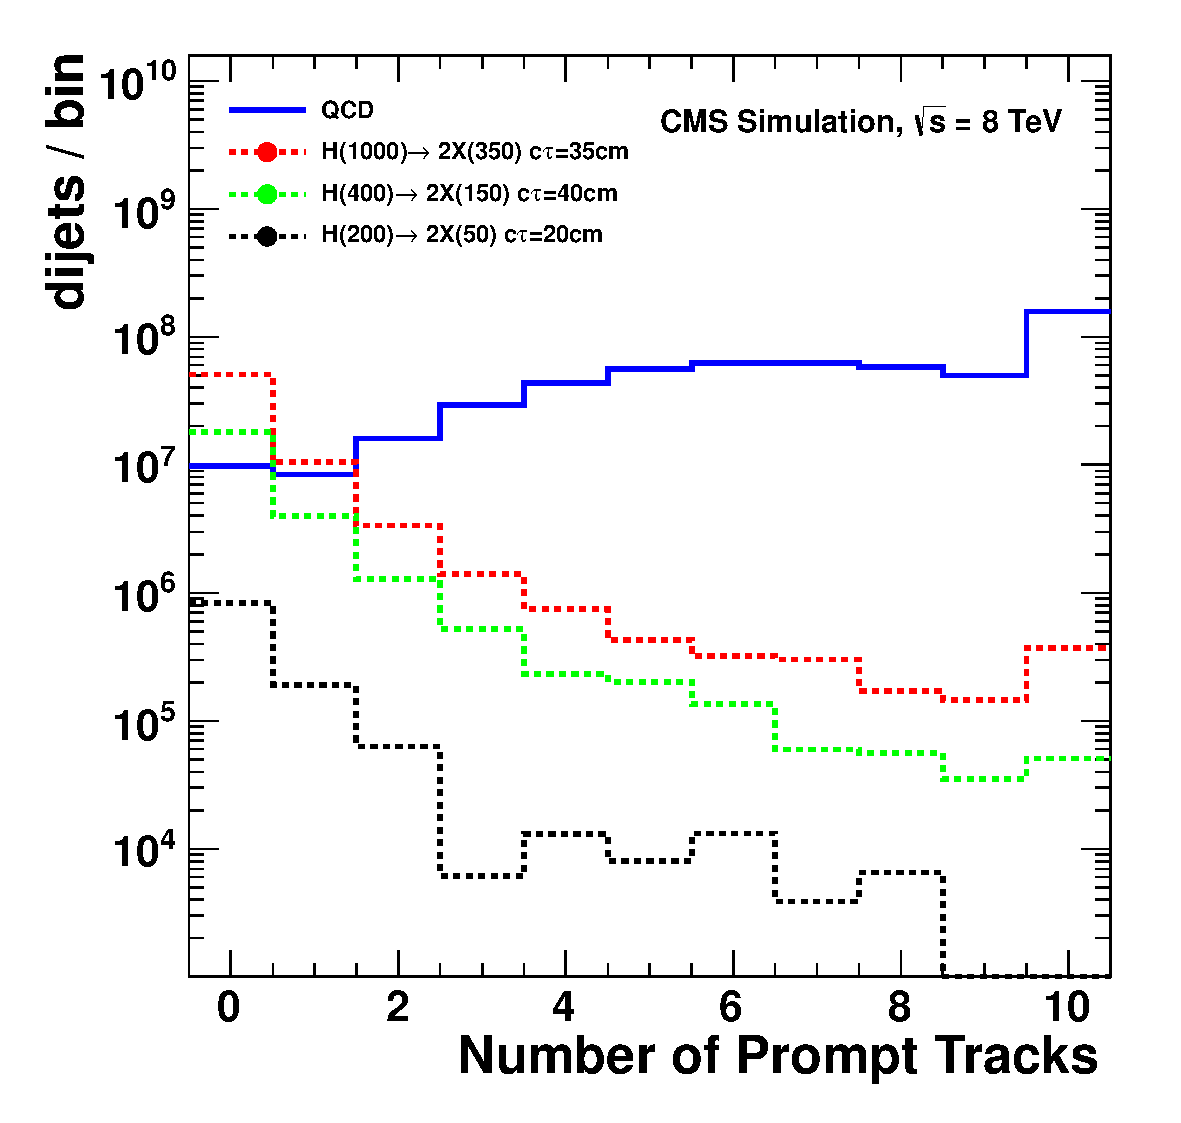
\includegraphics[width=0.49\textwidth]{plots/discrimination/disc_NPromptTracks.pdf}
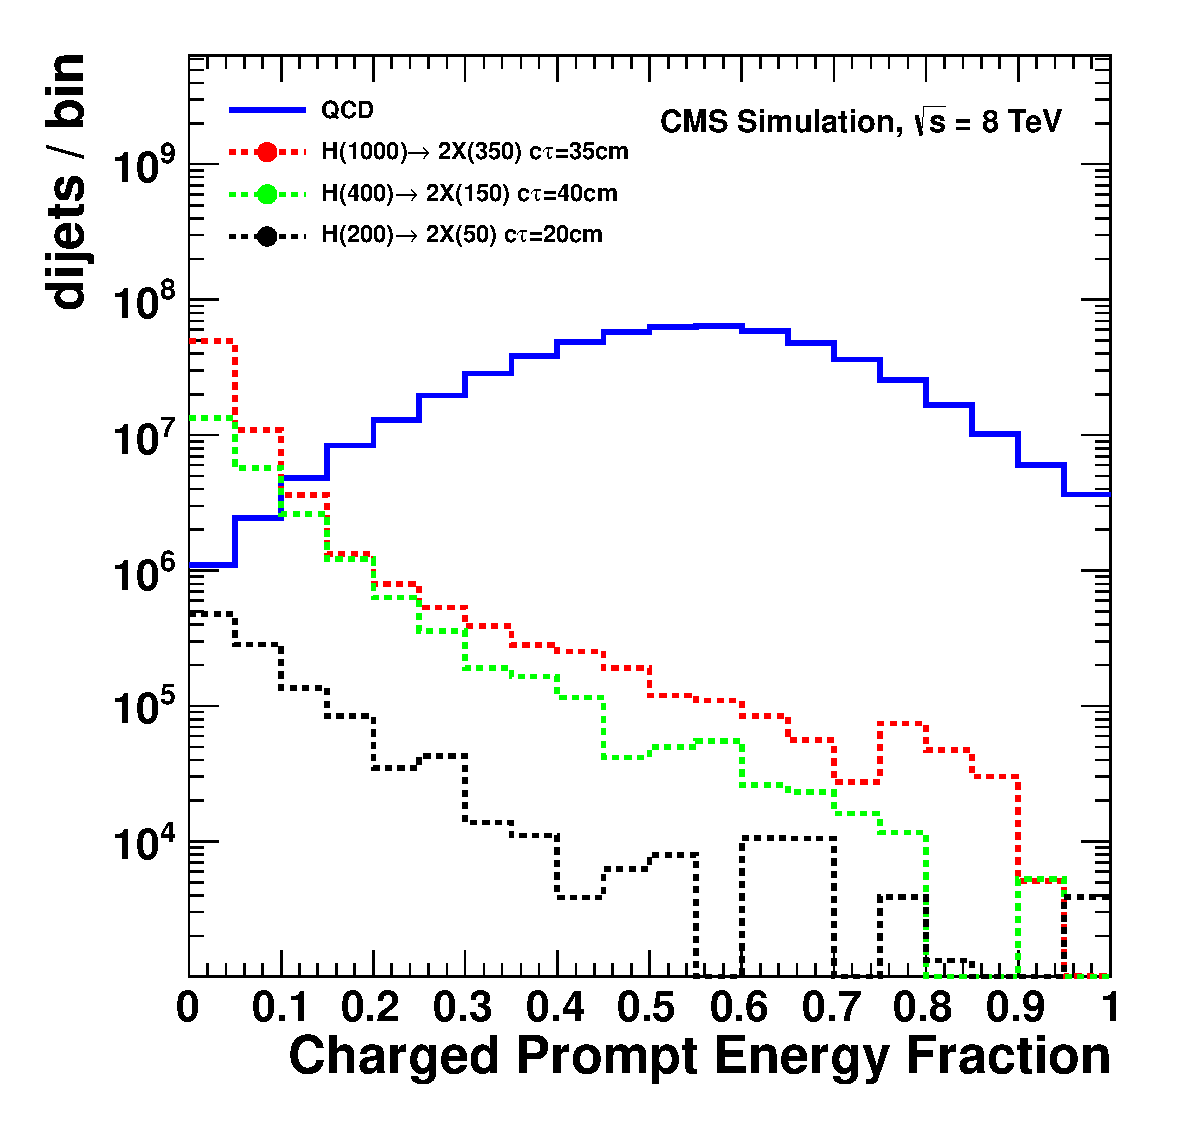
\includegraphics[width=0.49\textwidth]{plots/discrimination/disc_PromptEnergyFrac.pdf}
\caption{Number of prompt tracks associated to the jet and charged prompt jet energy fraction for signal and
background MC samples. There are two jets in a dijet pair, however the distributions for both jets are identical.
We present the distributions for the lower $p_T$ jet in the dijet pair.
\label{fig:discprompt}}

\end{figure}

Secondary vertices are searched among the tracks associated to each dijet pair 
using two different algorithms: 

\begin{enumerate}

\item{\bf Adaptive Vertex Fitter}
\label{subsec:AVF}
\cite{Waltenberger:1166320}. The secondary dijet vertex is required to have a chisquared per degree of freedom 
$\chi^2/dof < 5$. Additionally, for compatibility with the displaced dijet hypothesis we require that at least 
one track from each jet be included in the secondary vertex. 
This requirement greatly reduces the background contribution
from nuclear interaction vertices. The nuclear interaction vertices are characterized by low invariant mass
of the outgoing tracks, therefore it is unlikely that the outgoing tracks are associated to two distinct jets. 
The following quantities obtained from the vertex fit, with plots presented in Figure
\ref{fig:discvtx}, provide signal to background discrimination:
\begin{itemize}
 \item track multiplicity;
 \item fraction of tracks assigned to the vertex with a positive value of signed impact parameter;
 \item number of missing tracker hits behind the vertex position per track - each track in CMS is reconstructed 
from hits in the silicon tracker using a Kalman Filter algorithm \cite{Giordano:2012hr}. The algorithm propagates
 track seeds through the CMS tracker in the direction from the beam line towards the calorimeters. Whenever a hit 
is found along the trajectory the track parameters are updated, while occasional missing measurements 
are allowed. 
This variable represents an average count of missing tracker measurements 
starting from the fitted vertex position until the innermost hit of the vertex tracks. The fitted vertex position
may be significantly closer to the beam line than the track production point, if the track comes from a nuclear
 interaction or a $V^0$ decay;
 \item vertex invariant mass;
 \item vertex $p_T$;
 \item $L_{xy}$ significance - where $L_{xy}$ is the distance between secondary and primary vertices
in the transverse plane.
\end{itemize}


\begin{figure}
\centering
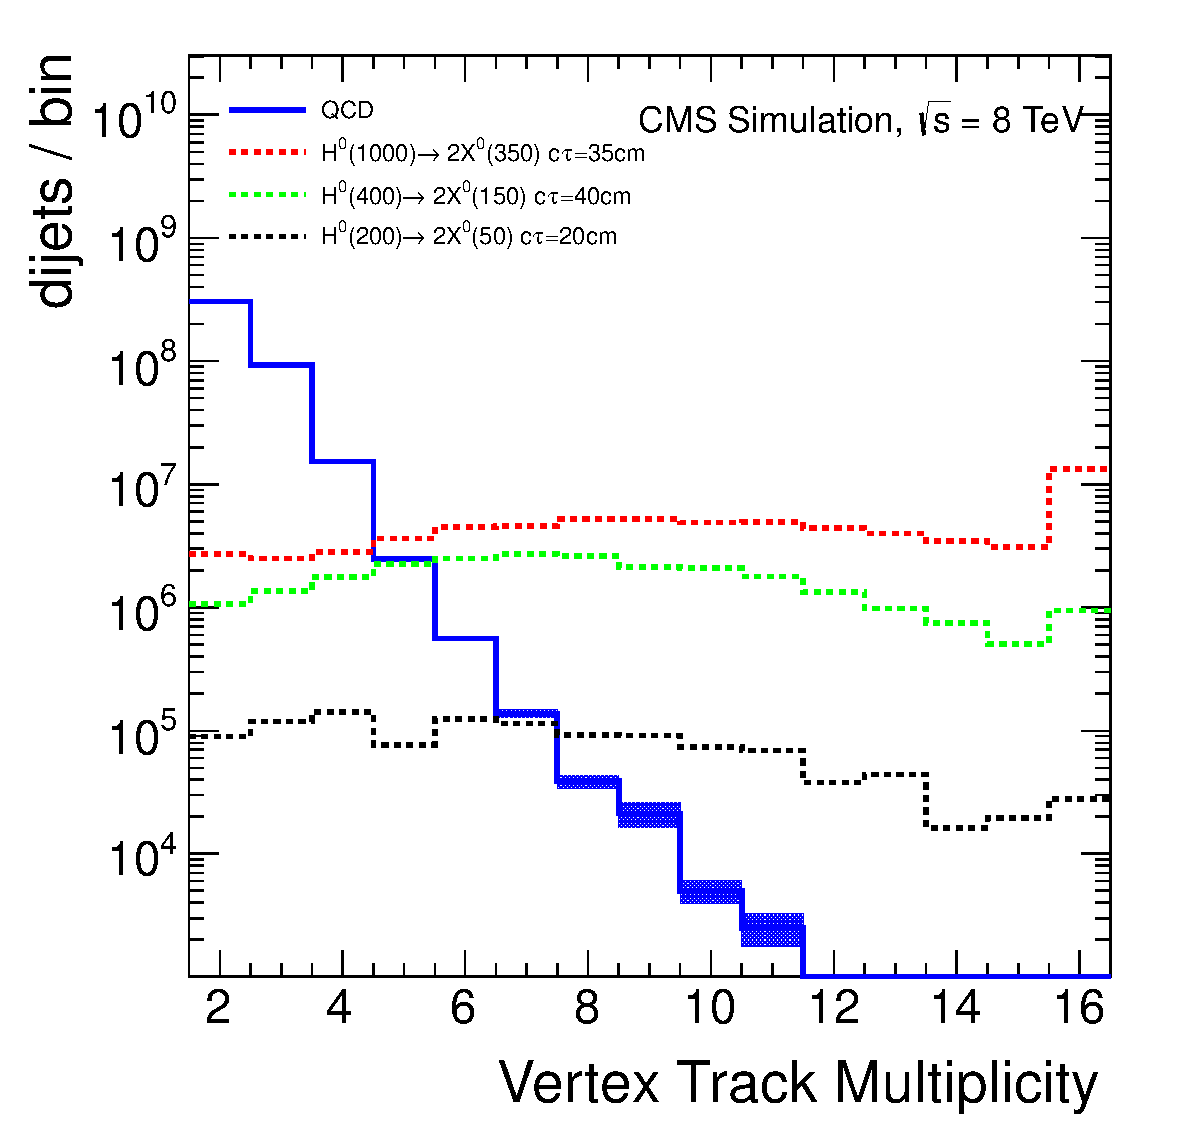
\includegraphics[width=0.49\textwidth]{plots/discrimination/disc_vtxN.pdf}
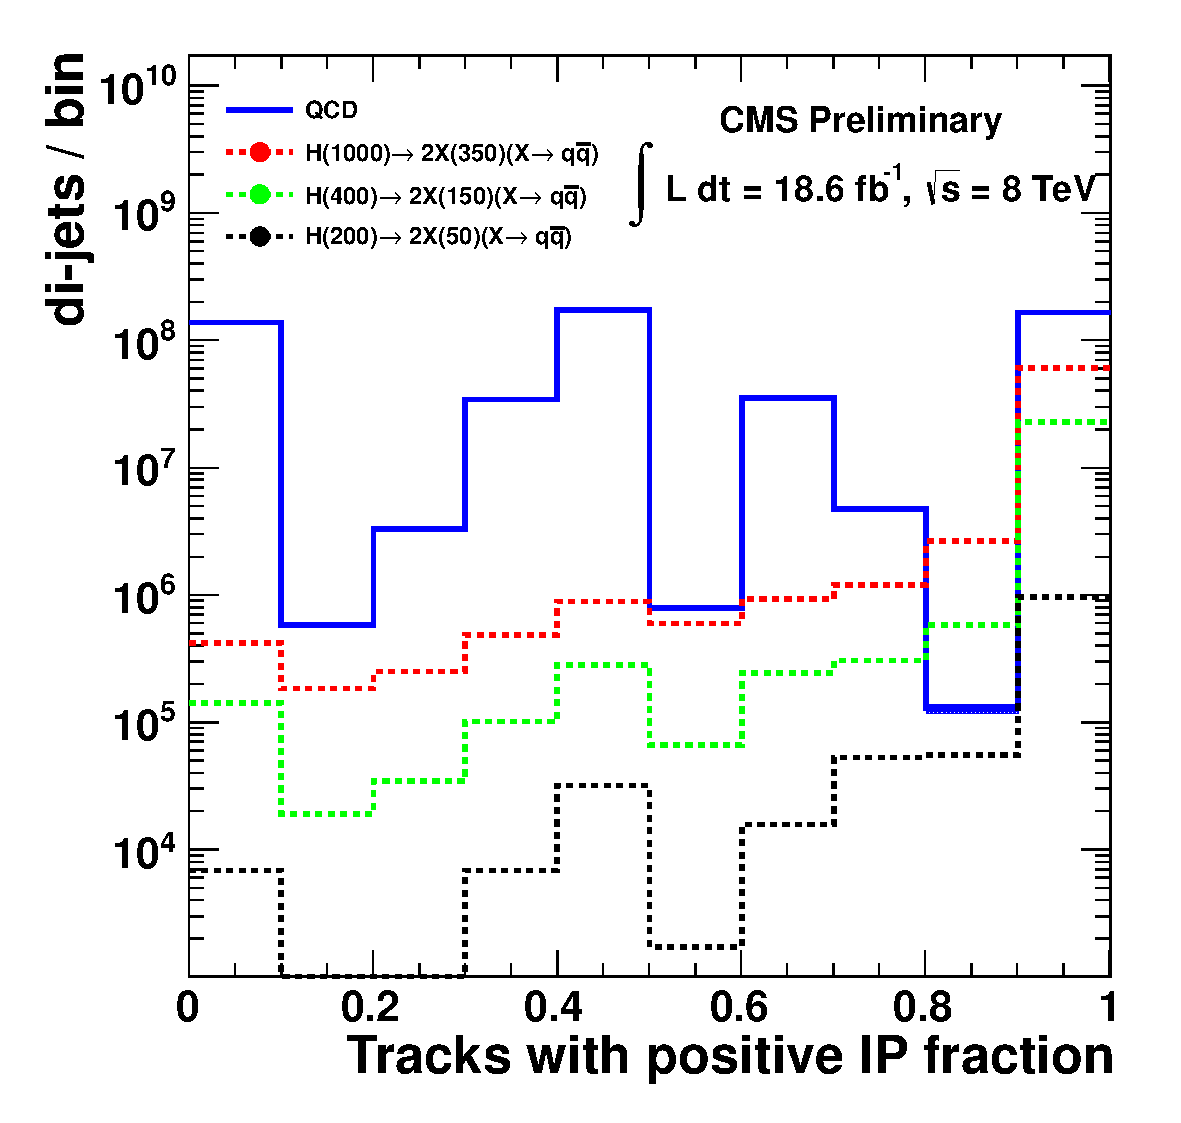
\includegraphics[width=0.49\textwidth]{plots/discrimination/disc_Posip2dFrac.pdf}
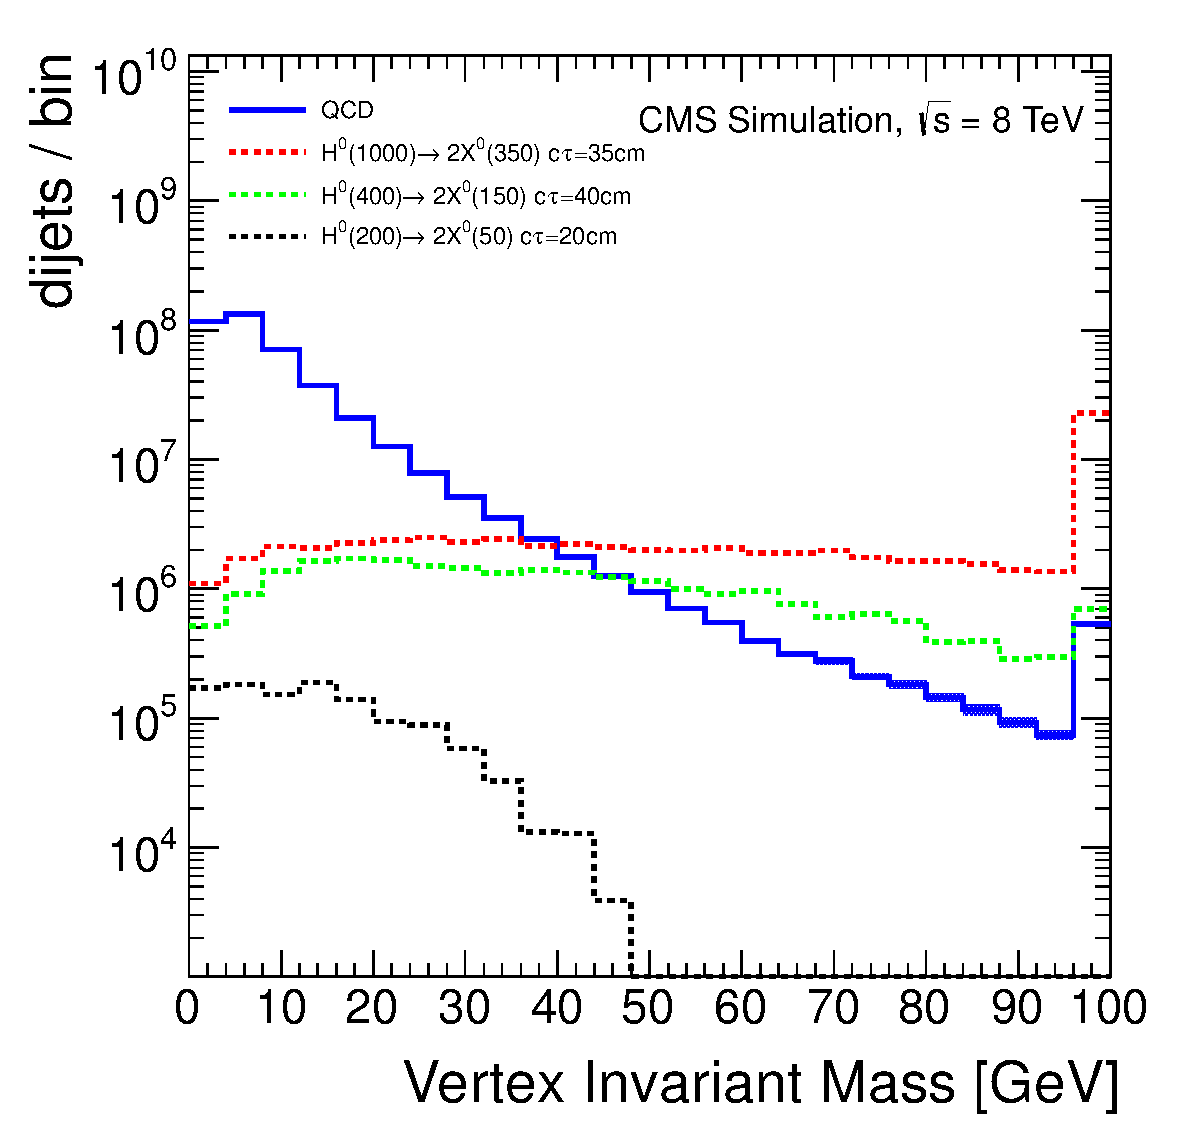
\includegraphics[width=0.49\textwidth]{plots/discrimination/disc_vtxmass.pdf}
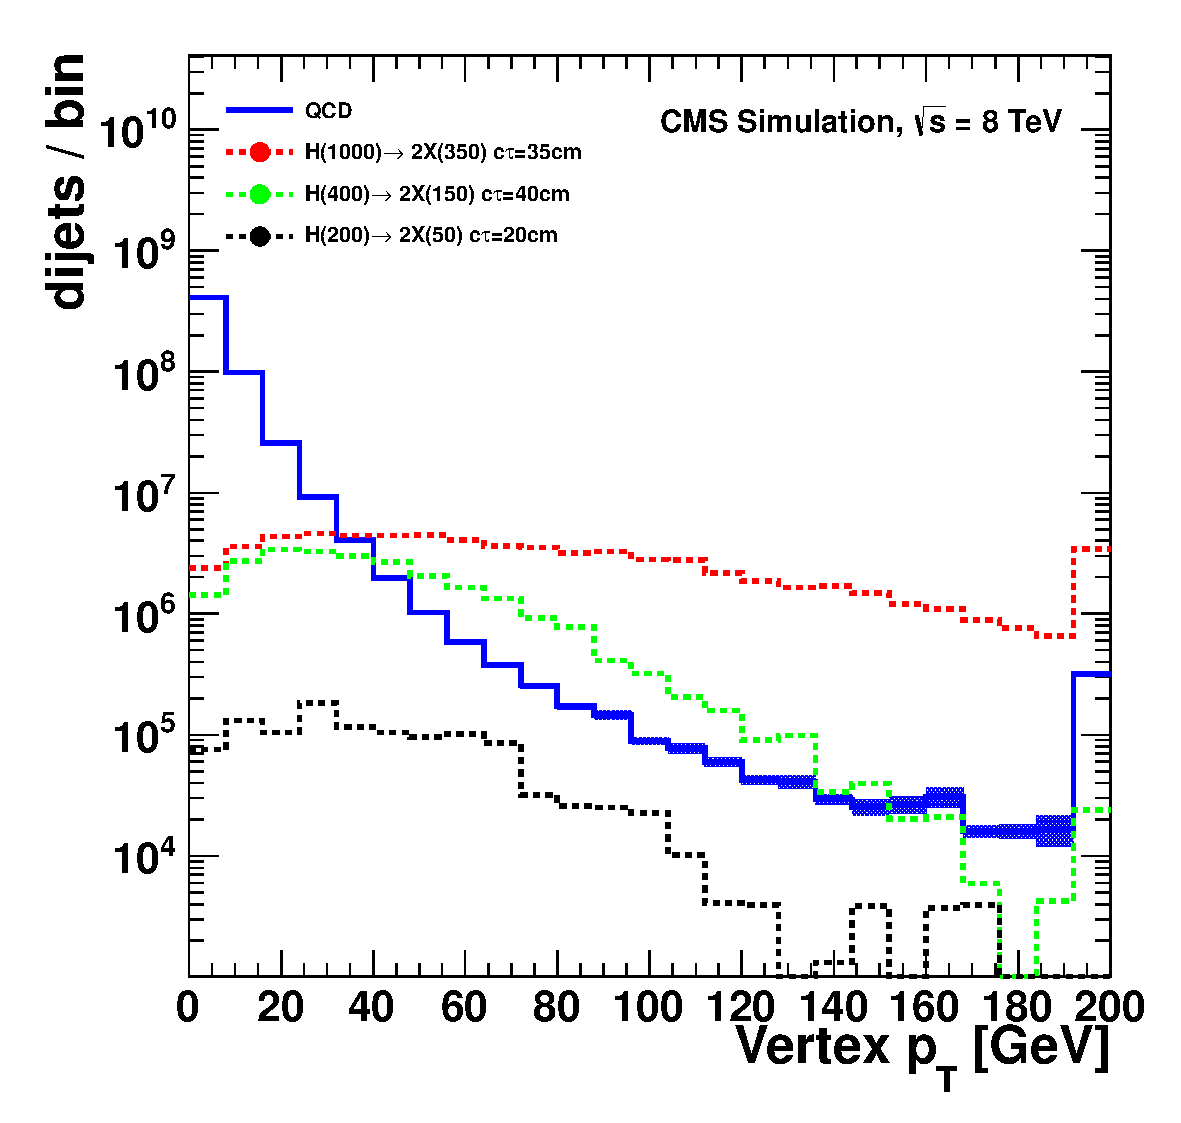
\includegraphics[width=0.49\textwidth]{plots/discrimination/disc_vtxpt.pdf}
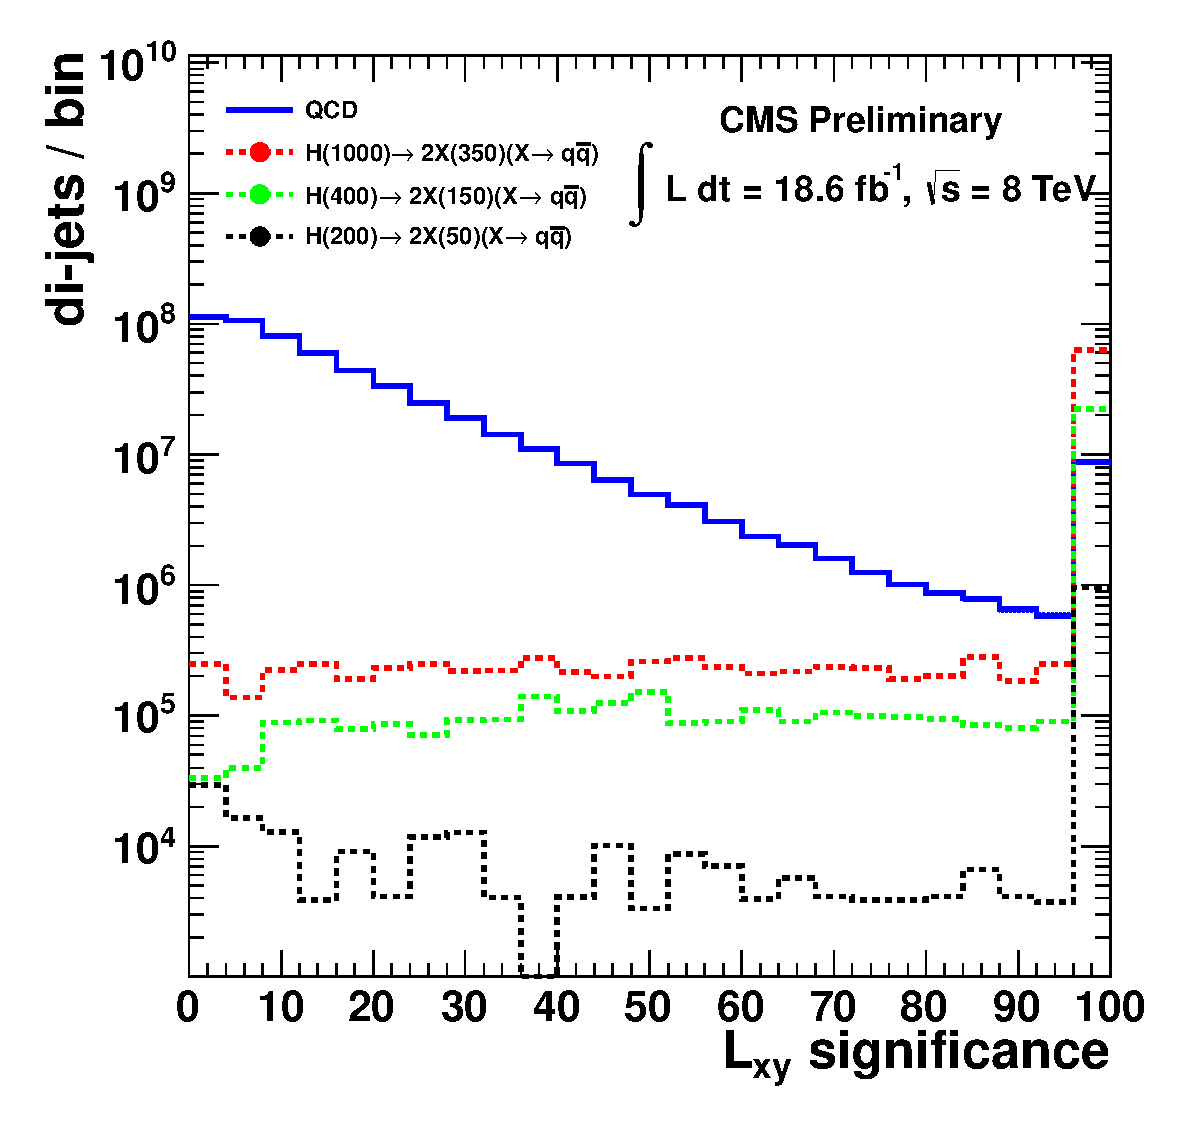
\includegraphics[width=0.49\textwidth]{plots/discrimination/disc_lxysig.pdf}
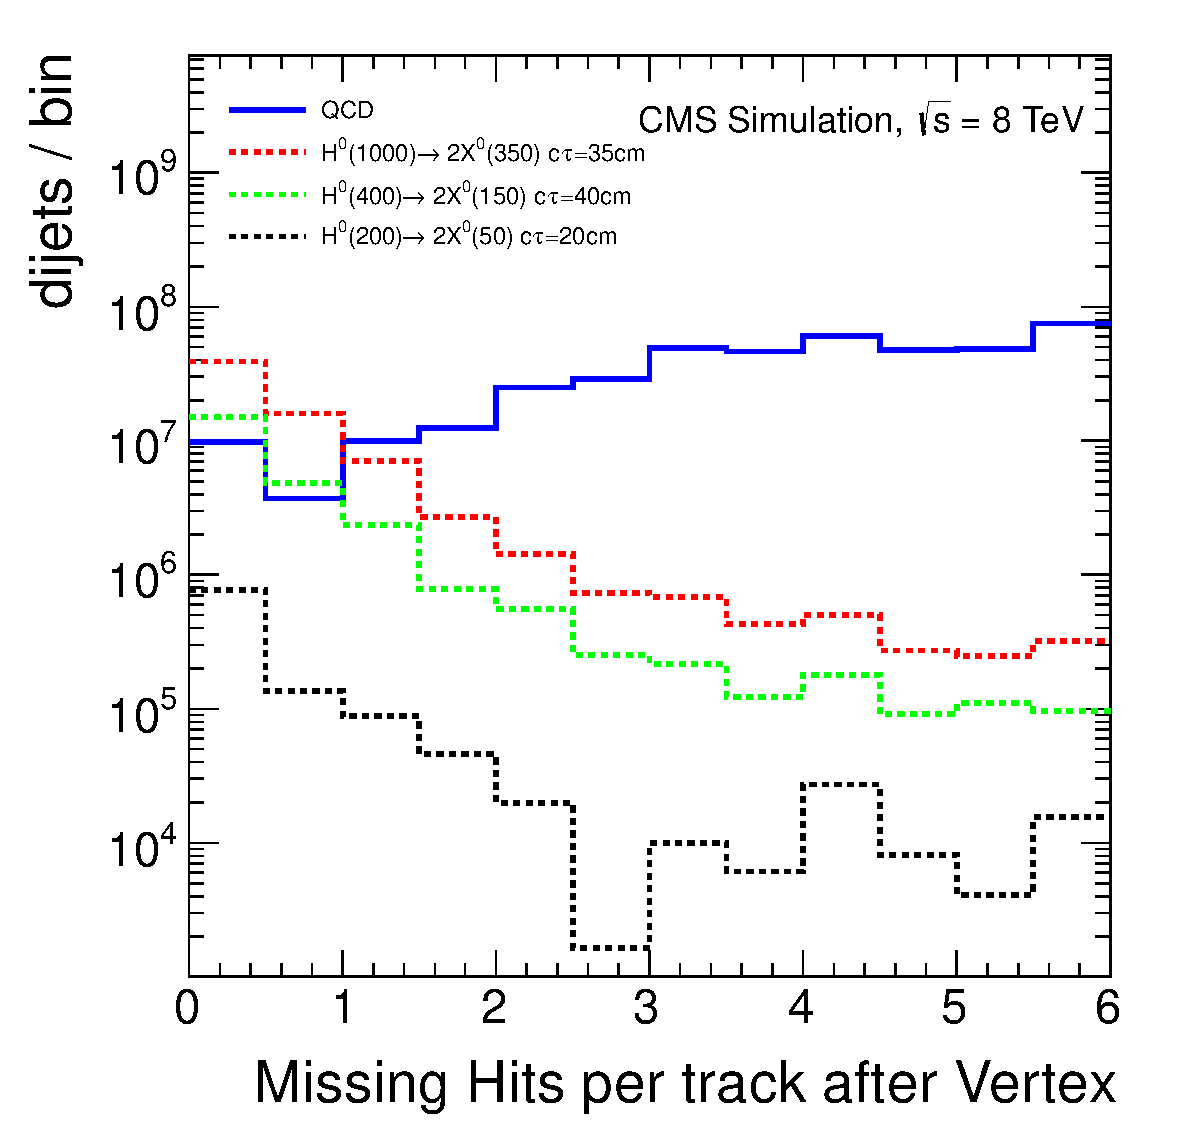
\includegraphics[width=0.49\textwidth]{plots/discrimination/disc_NAvgMissHitsAfterVert.pdf}
\caption{Secondary vertex discrimination variables for signal and background MC samples.\label{fig:discvtx}}

\end{figure}

\item{\bf Clusters of the expected path length}  
\label{subsec:Clusters}
- in this algorithm, for each of the displaced tracks associated to either jet a decay point consistent 
with the displaced dijet hypothesis 
is determined. As schematically presented in Figure 
\ref{fig:guesslxydiagram} such a point 
 can be obtained as the crossing point of   
the particle trajectory and a straight line drawn from the primary vertex in the direction of the dijet momentum.  
Information about the production point for each track is then used to compute an expected path length in the
transverse plane, $L_{xy}^{exp}$.  
For high momentum tracks the trajectory in the transverse plane is a straight line,
 therefore the decay point can be determined from the crossing point between two lines
 and the expected path length is simply:
\begin{equation}
 L_{xy}^{exp}=\frac{d_{xy}}{sin(\phi_{track} - \phi_{di-jet})}
\label{eqn:lxystraight}
\end{equation}
where $d_{xy}$ is the transverse impact parameter. However, in the presence of axial magnetic field 
the above formula is not valid due to track curvature. In order to find the expected path length in such case,
 we find a corresponding crossing point for the track helix with a radius $R$. Since we consider only
tracks with $p_T>$1\GeV which translates to the helix radius $R$ above 80\cm, 
the calculation is limited only to the first order in 
$d_{xy}/R$. 
 A line drawn from the primary vertex along the dijet momentum crosses the helix twice, yielding
 two solutions, although only one of them behaves properly when $R \to \infty$ 
and reduces to equation \ref{eqn:lxystraight}. Nevertheless, we consider two  
separate cases:
\begin{itemize}
 \item primary vertex lies inside the track helix:
\begin{equation}
 L_{xy}^{exp} = \frac{d_{xy}}{sin(\phi_{track} - \phi_{di-jet})} (1 - \frac{d_{xy}}{R}) + o((\frac{d_{xy}}{R})^2)
\end{equation} 
 \item primary vertex lies outside of the track helix:
\begin{equation}
 L_{xy}^{exp} = \frac{d_{xy}}{sin(\phi_{track} - \phi_{di-jet})} (1 + \frac{d_{xy}}{R}) + o((\frac{d_{xy}}{R})^2)
\end{equation} 
\end{itemize}
The difference between the two above cases lies only in the sign of the track curvature correction. This sign
however,  can be
determined from the track charge and the vector-product between the track transverse momentum vector and transverse
impact parameter vector:
\begin{equation}
q\cdot sgn((\vec{d_{xy}}\times\vec{p_T}) \cdot \vec{B})
\end{equation}   
where $\vec{B}$ vector is longitudinal. The final formula applied to each track is thus:
\begin{equation}
 L_{xy}^{exp} = \frac{d_{xy}}{sin(\phi_{track} - \phi_{di-jet})} (1 + q\cdot sgn((\vec{d_{xy}}\times\vec{p_T}) \cdot \vec{B}) \cdot \frac{d_{xy}}{R})
\label{eqn:lxy}
\end{equation}


\begin{figure}
\centering
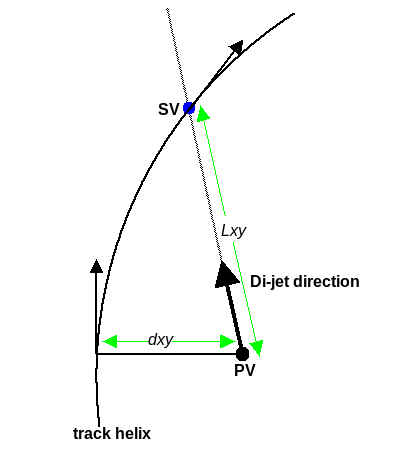
\includegraphics[width=0.3\textwidth]{plots/guessLxy.png}
\caption{Graphical representation of the crossing point (SV) between track helix and a straight line originating from the primary vertex (PV) in the direction of the dijet momentum. \label{fig:guesslxydiagram}}
\end{figure} 

For a genuine secondary vertex associated with a dijet pair the $L_{xy}^{exp}$ values obtained with equation
\ref{eqn:lxy} for each track should be close
 together, therefore we perform a 1-dimensional hierarchical clustering algorithm (appendix \ref{sec:hiercluster})
in order to select tracks belonging to the cluster. 
Clustering is performed with a size parameter equal to 15\% of 
the vertex $L_{xy}$ reconstructed with Adaptive Vertex Fitter. 
The tracks are added to the cluster given that the distances between the $L_{xy}^{exp}$
values are not larger than the size parameter. 
 If two or more clusters 
are reconstructed, the one closest to the vertex is selected. 
This algorithm is complimentary to Adaptive Vertex Fitter
since it uses additional information about the dijet direction. Discriminating variables provided
 by this algorithm include:
\begin{itemize}
\item cluster track multiplicity, Figure \ref{fig:discclr};
\item cluster RMS - a root-mean-square of the $L_{xy}^{exp}$ values belonging to the cluster
 relative to the vertex $L_{xy}$ given by Equation \ref{eqn:clrrms}. Additionally to cluster density, this
variable provides information whether both vertex and cluster reconstructions share the same tracks.
 If the two sets of tracks
are different that fact greatly increases the value of the cluster RMS, Figure \ref{fig:discclr}.
\begin{equation}
RMS_{cluster} = \sqrt{1/N_{tracks}\sum_{i=0}^{N_{tracks}}\frac{ (L_{xy}^{exp}(i) - L_{xy})^2}{L_{xy}^2}}
\label{eqn:clrrms}
\end{equation}
\end{itemize}

\begin{figure}
\centering
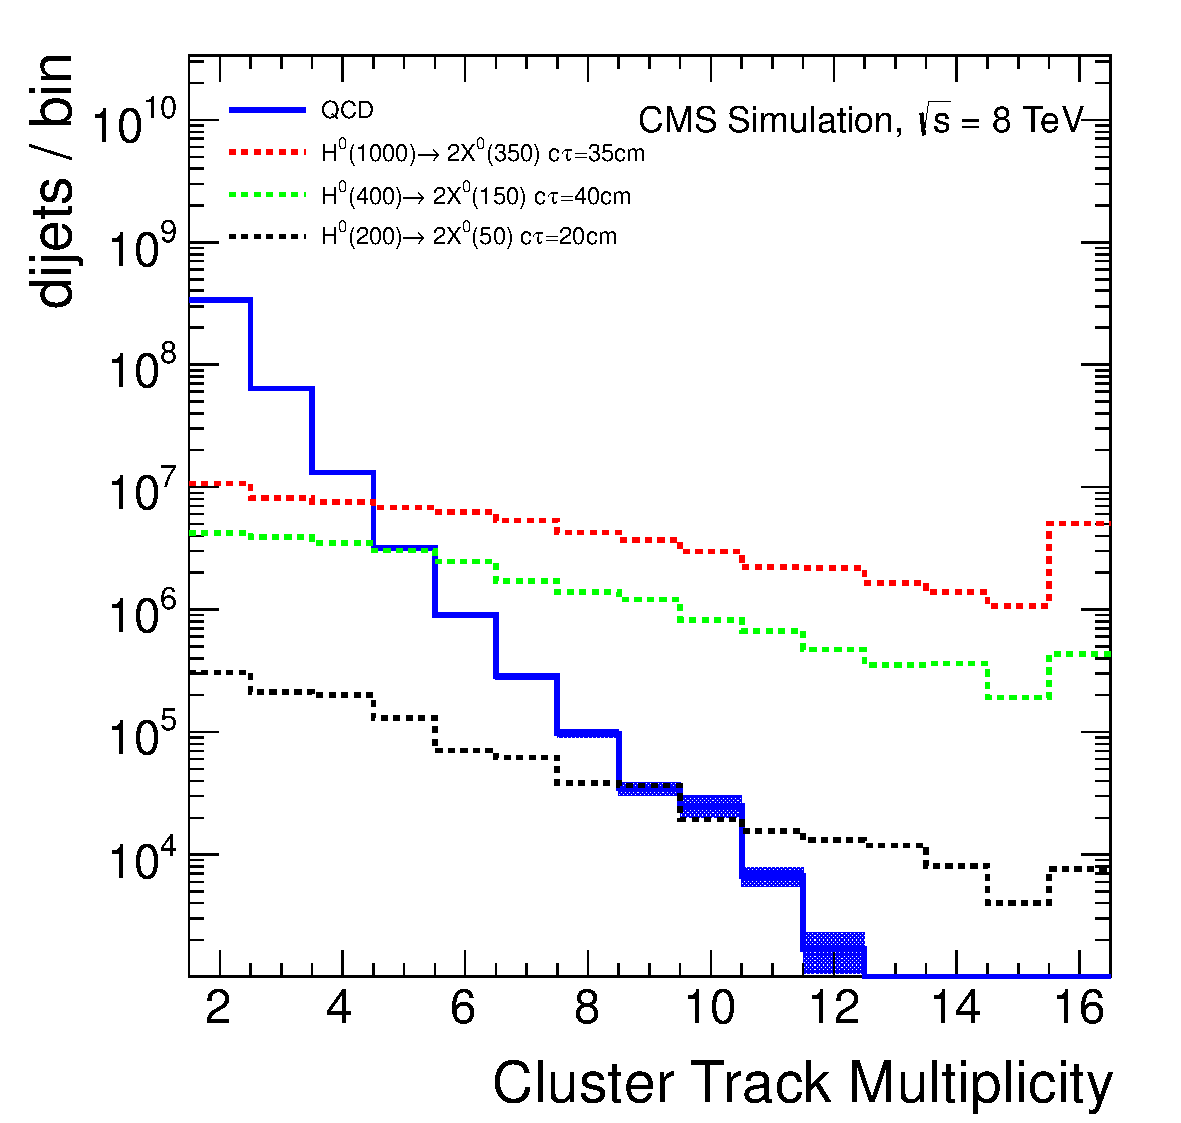
\includegraphics[width=0.49\textwidth]{plots/discrimination/disc_clrN.pdf}
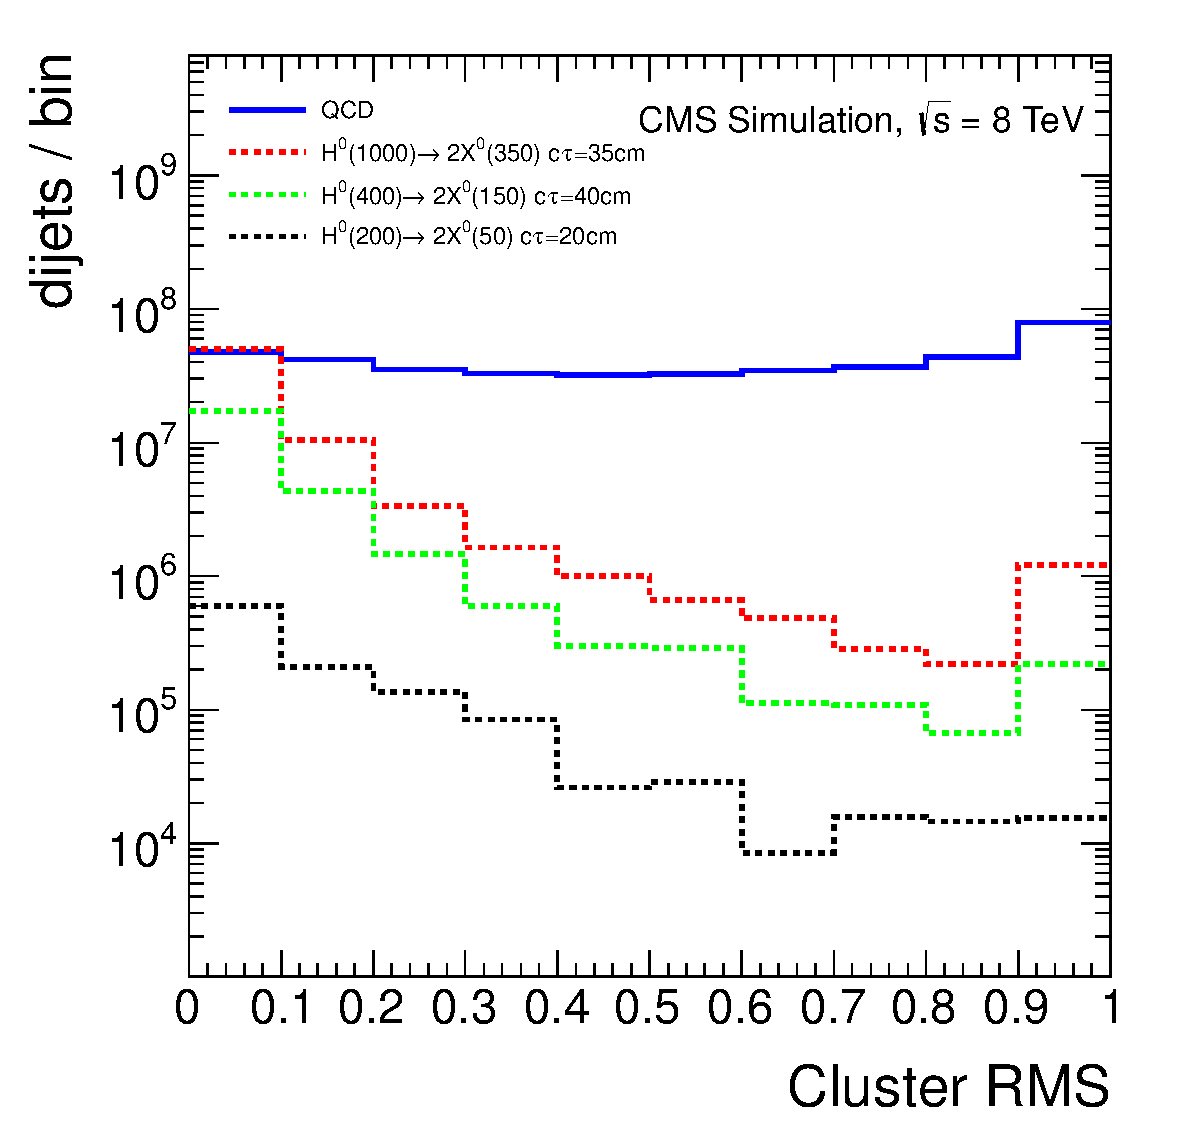
\includegraphics[width=0.49\textwidth]{plots/discrimination/disc_clrRMS.pdf}
\caption{Cluster discrimination variables for signal and background MC sample. \label{fig:discclr}}

\end{figure}


\end{enumerate}

\subsection{Selection}
\label{subsec:selection}

In this analysis  
to determine the background level we use a data driven technique
of independent selection criteria, the "ABCD method", which is
 described in detail in Section \ref{sec:background}. This method requires
at least two selection criteria where the probability of a background candidate to pass one of the criteria is
not strongly correlated with whether it passes the other criteria. Such selection criteria can be generally
constructed
from variables which are mutually independent. 
 In order to eliminate pairs of variables that are not independent,
 correlation factors have been studied using the background samples.  
Correlation factors between variables $x$ and $y$ are obtained from binned two-dimensional histograms 
according to the formula:
\begin{equation}
 corr(x,y) = cov(x,y)/RMS(x)RMS(y), \hspace{5pt} cov(x,y)= \sum_i(x_i y_i)/N - \sum_i(x_i)/N \sum_i(y_i)/N
\label{eqn:corr}
\end{equation}
where N is the normalization of the histogram and index i loops over the histogram bins. Based on the study of the correlation factors, we construct
3 independent selection criteria for the background estimation:

\begin{itemize}     
\item[Selection 1.] {\bf Combination of the number of prompt tracks and prompt tracks jet energy fraction selections} - for first jet in the dijet pair;
\item[Selection 2.] {\bf Combination of the number of prompt tracks and prompt tracks jet energy fraction selections} - for second jet in the dijet pair;
\item[Selection 3.] {\bf Combined vertex \& cluster likelihood discriminant}. 
We select variables which have small model dependence and are 
well uncorrelated with prompt tracks variables. They include:
\begin{itemize}
 \item vertex track multiplicity;
 \item fraction of tracks assigned to the vertex with positive value of signed transverse impact parameter;
 \item cluster track multiplicity;
 \item cluster RMS.
\end{itemize}  
The likelihood discriminant is obtained using signal and background Monte Carlo samples, where samples for
various signal models are added together due to small signal dependence of the variables used.
For each dijet candidate a signal probability is computed according to the formula:
\begin{equation}
p=\frac{p_S}{p_S+p_B}=\frac{1}{1+p_B/p_S}=\frac{1}{1+\Pi_i p_B{}_i/p_S{}_i}
\label{eqn:likelihood}
\end{equation}
where i index loops over variables included in the discriminant. The correlations between individual variables 
within the discriminant are
neglected. Individual probability densities are determined 
using 1-dimensional histograms for signal and background candidates separately.
\end{itemize}

As presented in Table \ref{tab:corr}, the individual correlation factors between the variables used for background
estimation do not exceed a few percent level in the background MC samples.
There are large correlations between number of prompt tracks and jet energy fraction carried by prompt tracks 
for the same jet, hence these two selections are applied together, while there is very little correlation for these
variables between the two jets which form the dijet pair. The choice of variables is additionally motivated
 by the fact
that the prompt track variables are independent between the two jets due to lack of standard model 
process giving rise
to displaced dijet pairs, while the variables associated with the secondary vertex use displaced tracks
from both jets simultaneously.    

\begin{table}[htbp]
\centering
\caption{Correlation factors obtained with equation \ref{eqn:corr} between the variables 
used for background estimation obtained from background QCD Monte
Carlo samples. N1 and N2 represent the numbers
of prompt tracks for jet 1 and 2 respectively, while fraction 1 and 2 the jet energy fraction carried by 
prompt tracks.
\label{tab:corr}}
\begin{tabular}{c|ccccc}
 & Vtx/Cluster & N1 & N2 & fraction 1 & fraction 2 \\
\hline
Vtx/Cluster & - & 1.1\% & 2.5\% & -2.7\% & 1.8\%  \\
N1 & & - & 2.3\% & 26\%  & 1.2\% \\
N2 & & & - & 0.5\% & 31\% \\
fraction 1 & & & & - & 0.3\% \\
fraction 2 & & & & & - \\
\end{tabular}
\end{table}

The final selection criteria on the variables used for background estimation are described in Section 
\ref{subsec:cutvalues}. For all remaining discrimination variables we require loose pre-selection criteria:   
\begin{itemize}
 \item vertex invariant mass $>$ 4\GeV;
 \item vertex $p_T>$ 8\GeV;
 \item average number of missing tracker hits behind the secondary vertex position $\leq$ 2 per track;
 \item $L_{xy}$ significance $>$ 8.
\end{itemize}

In case a single jet is used in more than one di-jet pair after pre-selection, we resolve
the ambiguity by choosing the highest $L_{xy}$ significance candidate for each jet, thus ensuring that
each jet is only used once. 

Pre-selection criteria efficiencies are presented in Table \ref{tab:seleff}.  
When the pre-selection requirements are applied to each dijet candidate,
the efficiencies are computed using the number of events with at least one candidate fulfilling the selection.
The requirement for the signal candidates to be matched with a decay of an \X boson at the generator level,
 denoted in Table \ref{tab:seleff} as {\it signal dijet}, 
is inefficient with respect to the trigger, if the two triggering
jets do not originate from the same \X boson particle.  
The $H_T>300\GeV$ requirement imposed by the trigger reduces the efficiency for lower masses of the \Higgs, 
while the vertex reconstruction efficiency is affected by the acceptance of the CMS tracker, which cannot 
reconstruct vertices displaced by more than 60\cm in the transverse plane. However, if the trigger accepted a signal event and the secondary vertex is reconstructed
for at least one of the \X boson candidates the pre-selection criteria efficiency is high for the signal samples
when compared to the background.   

\begin{table}[!htbp]
\centering
\caption{Trigger and pre-selection criteria efficiency for data,
background Monte Carlo and three selected signal models. 
Event selection efficiencies in each row are relative to events that passed the criteria from rows above.
All criteria, except the trigger, are applied to individual dijet candidates.
There may be many dijet candidates in a single event, therefore
for those criteria the efficiency is computed using the number of events 
containing at least one dijet candidate that fulfills the selection. 
\label{tab:seleff}}
\begin{tabular}{lccccc}
%\hline
 & \multicolumn{5}{c}{pre-selection criteria efficiency} \\
\cline{2-6}
 & & &  $M_H$=1000\GeV & $M_H$=400\GeV & $M_H$=200\GeV \\
 & & &  $M_X$=350\GeV & $M_X$=150\GeV & $M_X$=50\GeV \\
selection & data & bkg. MC & $c\tau$=35\cm & $c\tau$=40\cm & $c\tau$=7\cm\\
\hline
trigger & - & 0.01\% & 97\% & 53\% & 3.9\% \\
has dijet & 99\% & 99\% & 100\% & 100\% & 99\% \\
signal dijet & - & - & 88\% & 65\% & 21\% \\
has vertex & 25\% & 24\% & 69\% & 59\% & 61\% \\
has cluster &  72\% & 72\% & 99\% & 98\% & 98\% \\
\hline
vertex $\chi^2$ & 93\% & 93\% & 100\% & 99\% & 99\% \\
vertex mass &  78\% & 82\% & 98\% & 97\% & 74\% \\
vertex $p_T$ & 43\% & 42\% & 97\% & 95\% & 92\% \\
max missing hits & 8.5\% & 12\% & 98\% & 98\% & 98\%  \\
$L_{xy}$ significance & 78\% & 68\% & 100\% & 100\% & 100\% \\
\hline 
\end{tabular}
\end{table}

In order to validate the simulation based study we compare the data and background MC distributions
in a control region for candidates passing the pre-selection.
We use a control region that requires passing the single jet trigger
(HLT\_HT300\_SingleDisplacedPFJet60) and vetoes events passing the double jet trigger
 (HLT\_HT300\_DoubleDisplacedPFJet60). Compared to the signal region, there is a factor of 100 less instantaneous 
luminosity and the signal efficiency for all considered signal models is at least factor of 10 less
compared to the efficiency
in the signal region. Plots \ref{fig:promptness}, \ref{fig:discriminant}, \ref{fig:vertex} 
and \ref{fig:cluster} present all 
discrimination variables used in the analysis in the control region
after candidate pre-selection. The {\it number of missing hits per track after vertex} requirement has been removed
in order to increase the statistics of the 
data and background Monte Carlo samples. 
%Good agreement between data and background Monte Carlo is found. 

\begin{figure}[htbp]
\centering
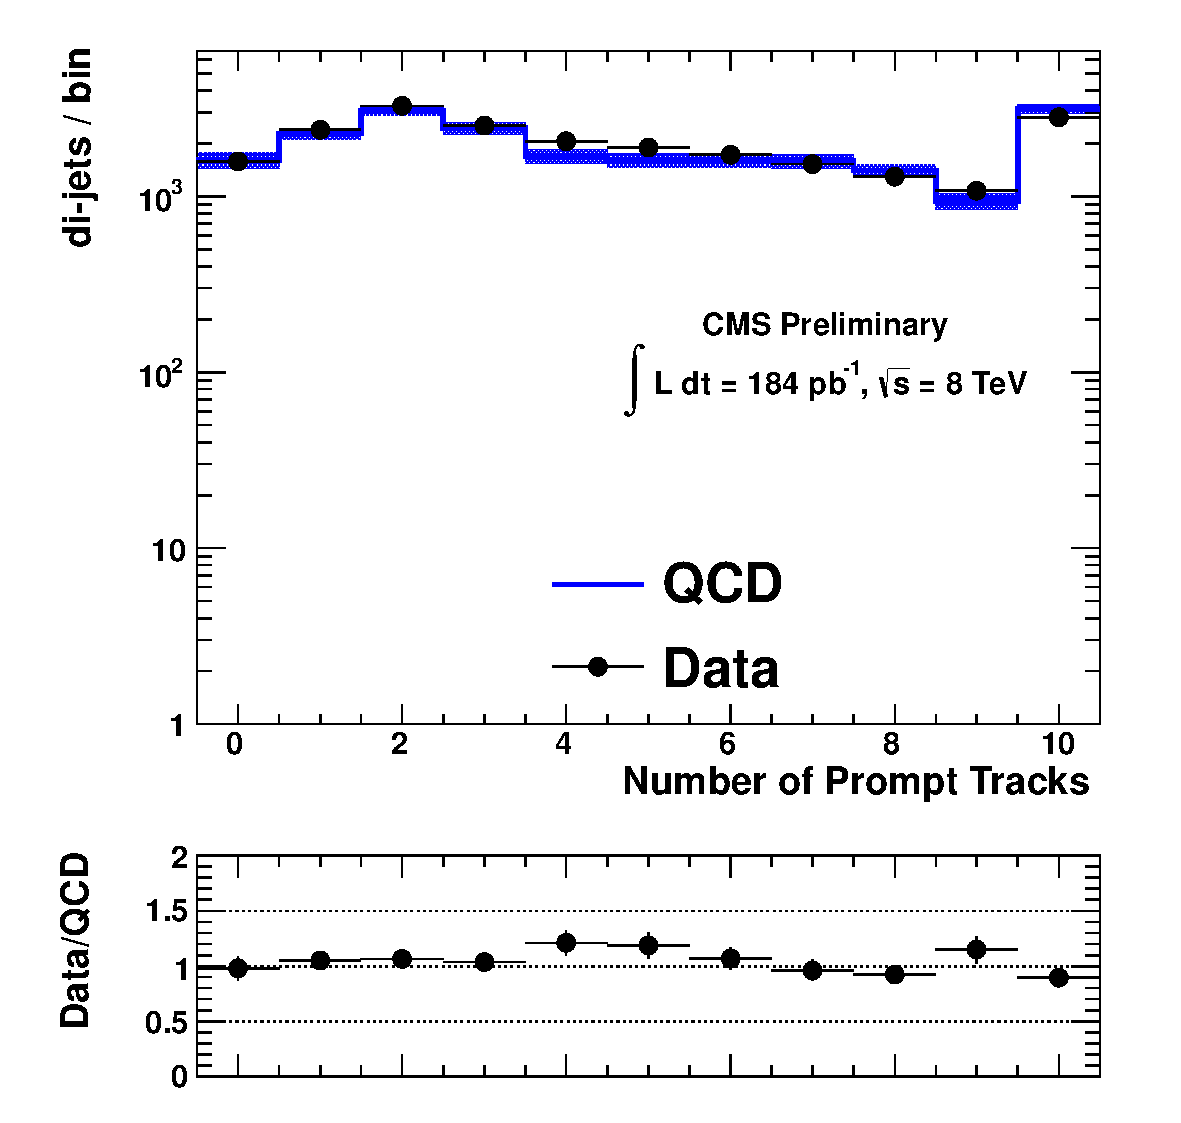
\includegraphics[width=0.49\textwidth]{plots/control/ctrl_NPromptTracks.pdf}
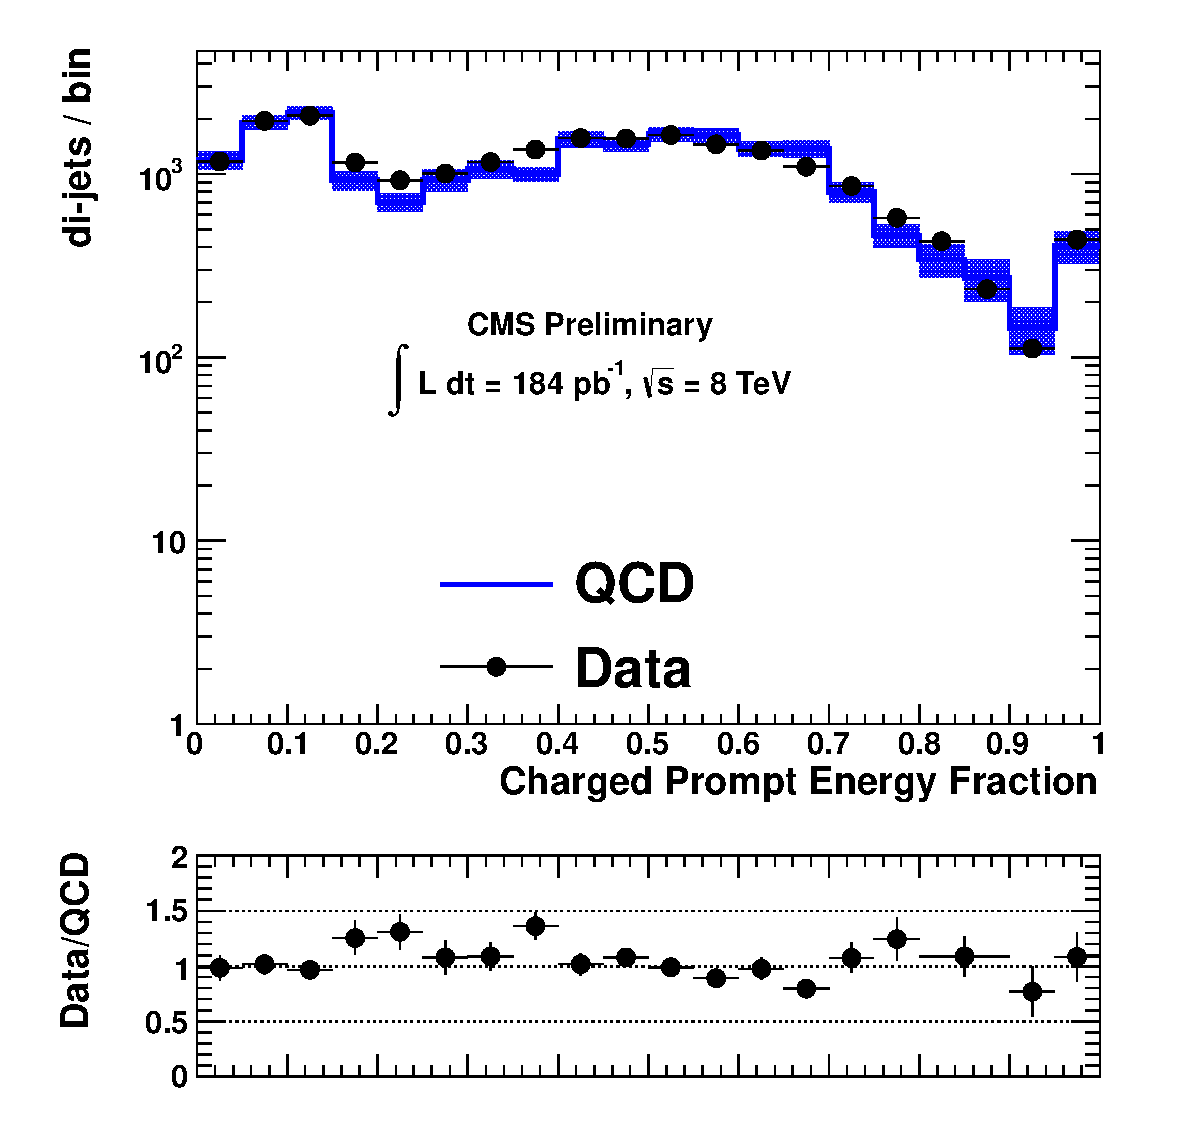
\includegraphics[width=0.49\textwidth]{plots/control/ctrl_PromptEnergyFrac.pdf}

\caption{Prompt track variables corresponding to the ones used in the trigger. 
The characteristic shape towards low values in both variables
shows the contribution of jets passing the non-prompt trigger requirement. \label{fig:promptness}}
\end{figure}

\begin{figure}[htbp]
\centering
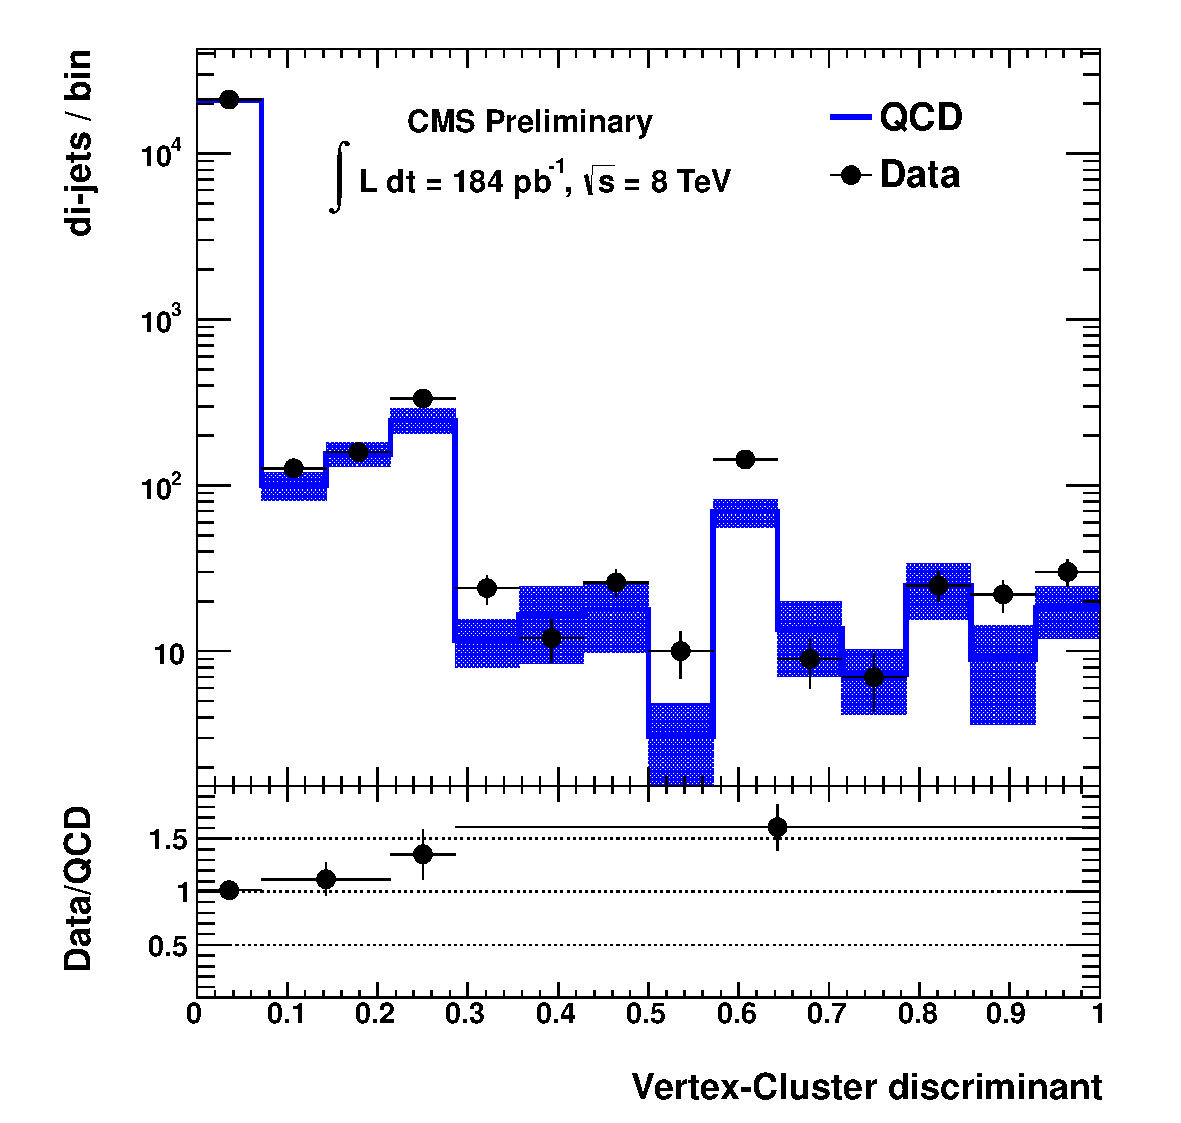
\includegraphics[width=0.49\textwidth]{plots/control/ctrl_Discriminant.pdf}
\caption{Vertex-Cluster likelihood discriminant.\label{fig:discriminant}}
\end{figure}

\begin{figure}[htbp]
\centering
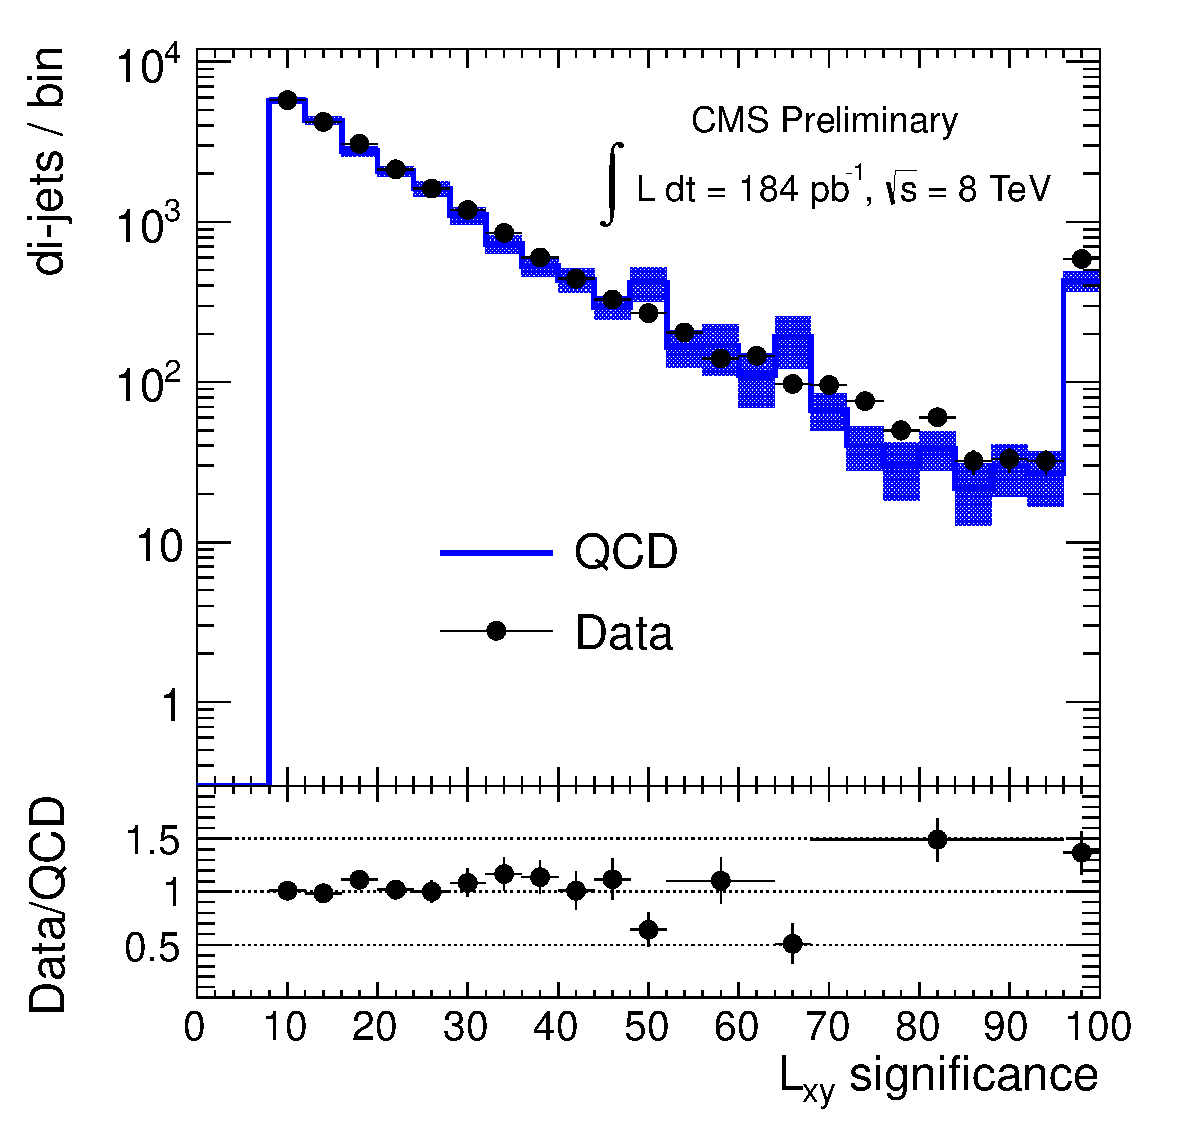
\includegraphics[width=0.49\textwidth]{plots/control/ctrl_Lxysig.pdf}
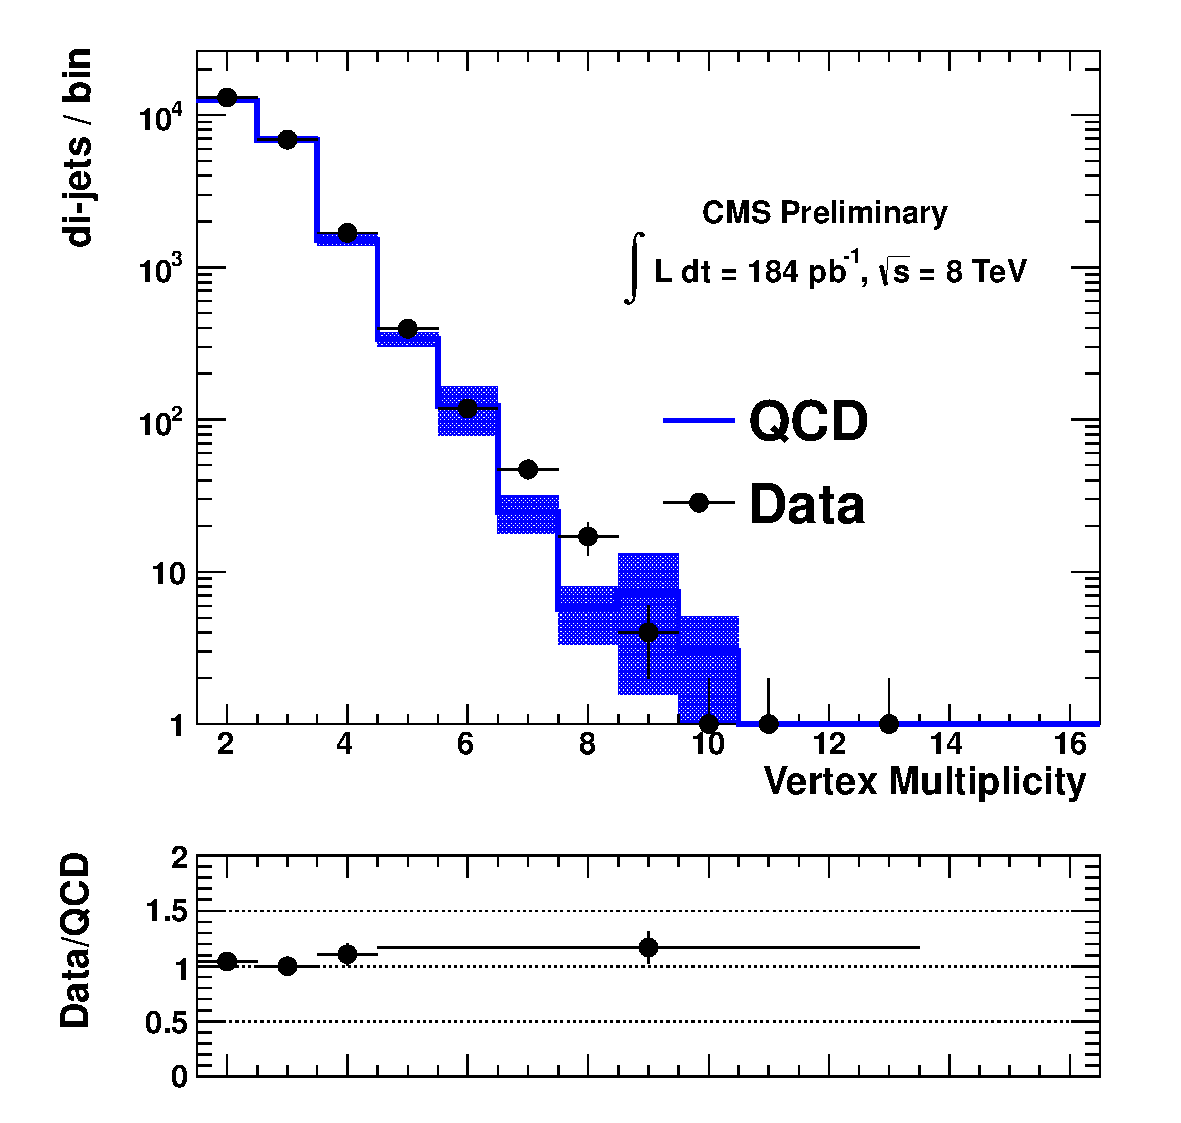
\includegraphics[width=0.49\textwidth]{plots/control/ctrl_VtxN.pdf}\\
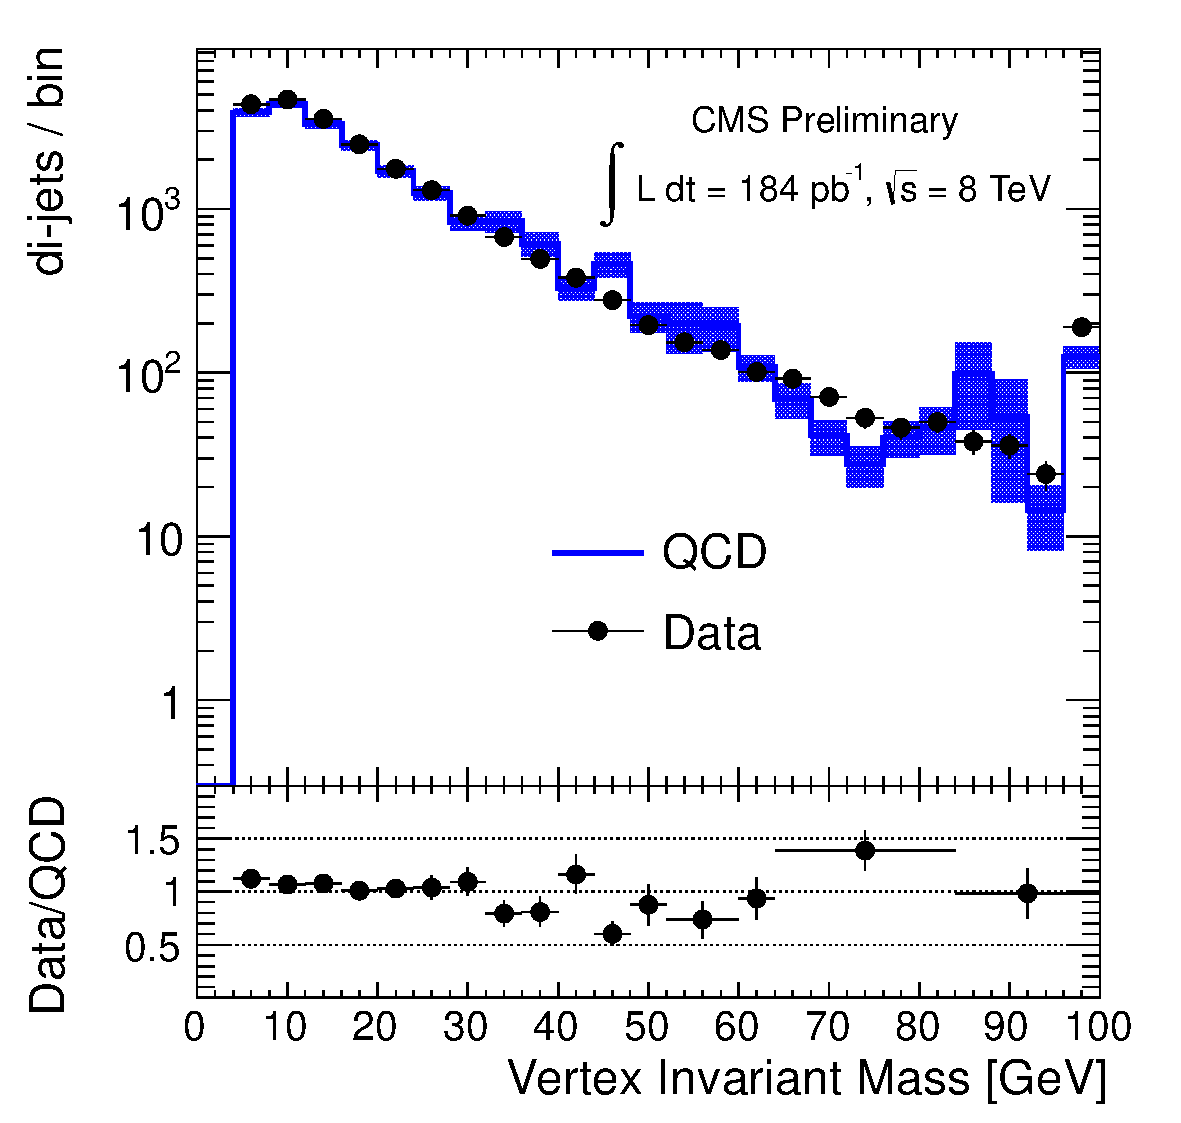
\includegraphics[width=0.49\textwidth]{plots/control/ctrl_Vtxmass.pdf}
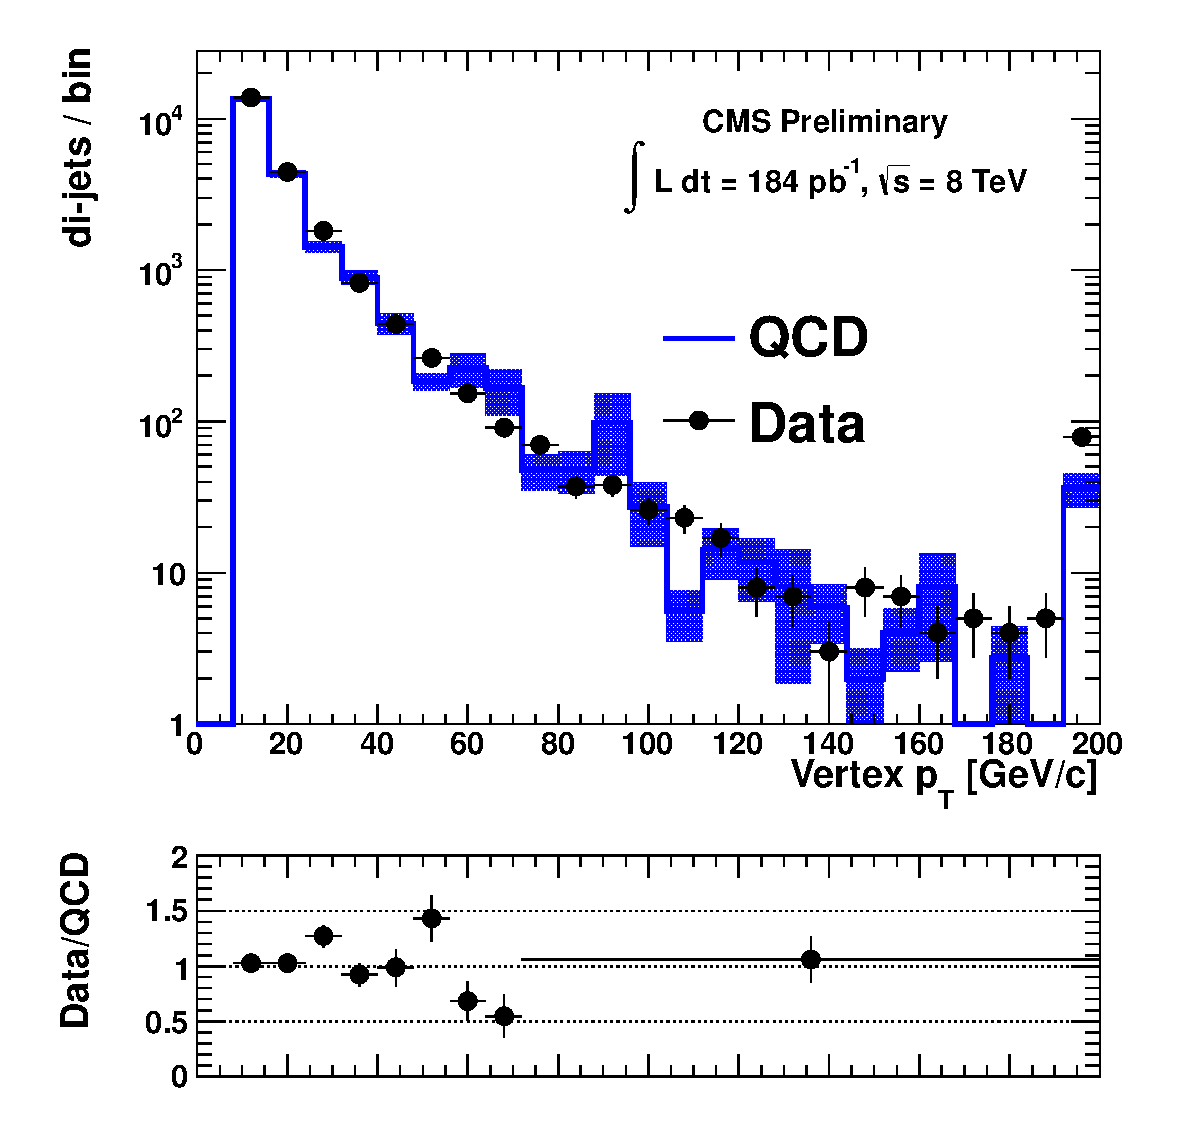
\includegraphics[width=0.49\textwidth]{plots/control/ctrl_Vtxpt.pdf}\\
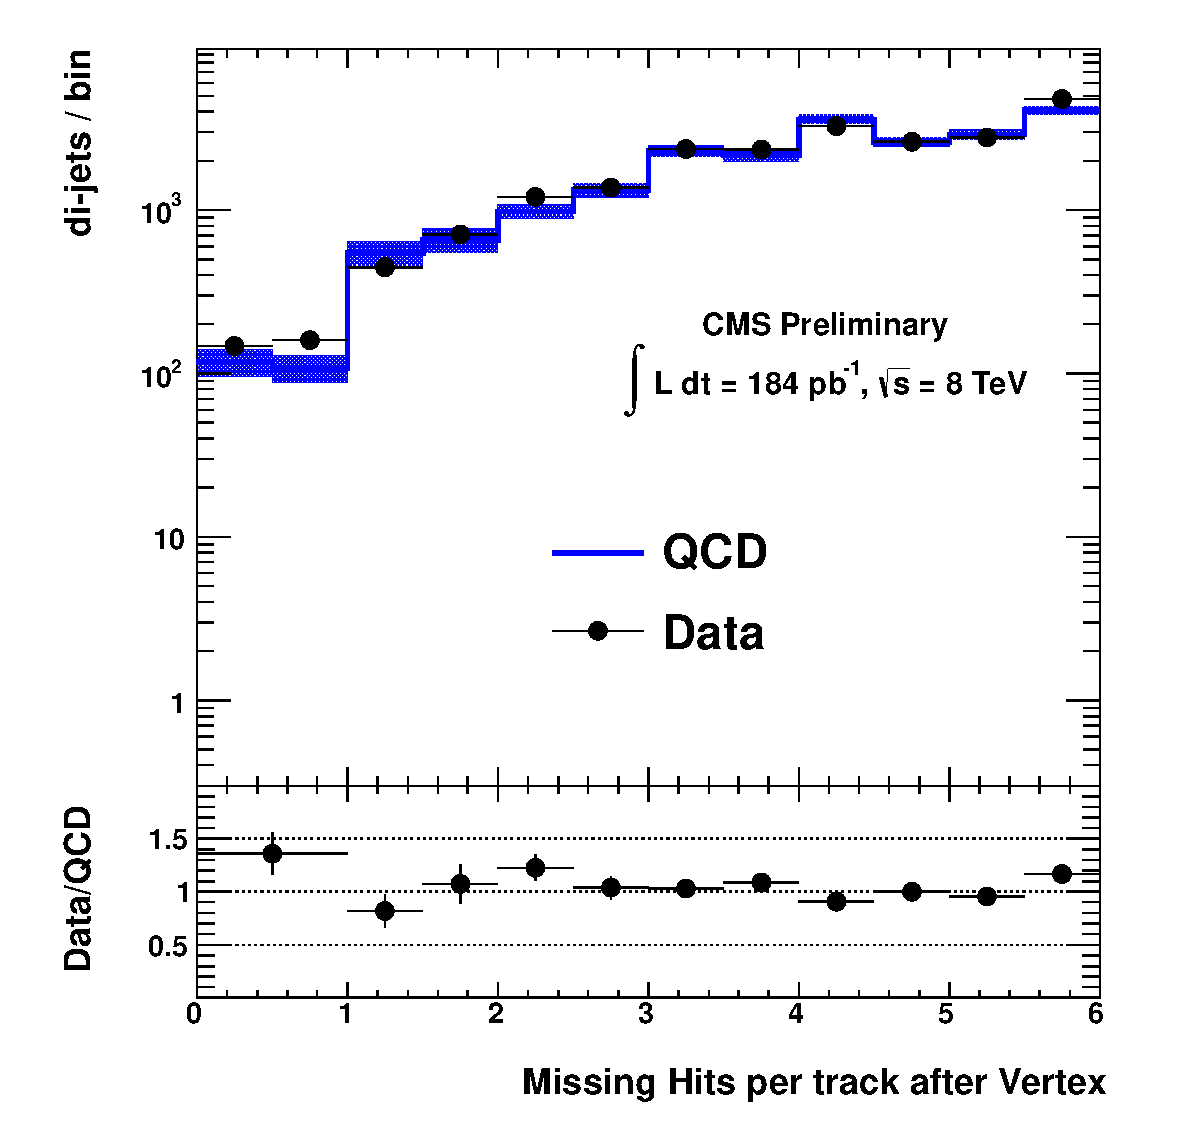
\includegraphics[width=0.49\textwidth]{plots/control/ctrl_NAvgMissHitsAfterVert.pdf}
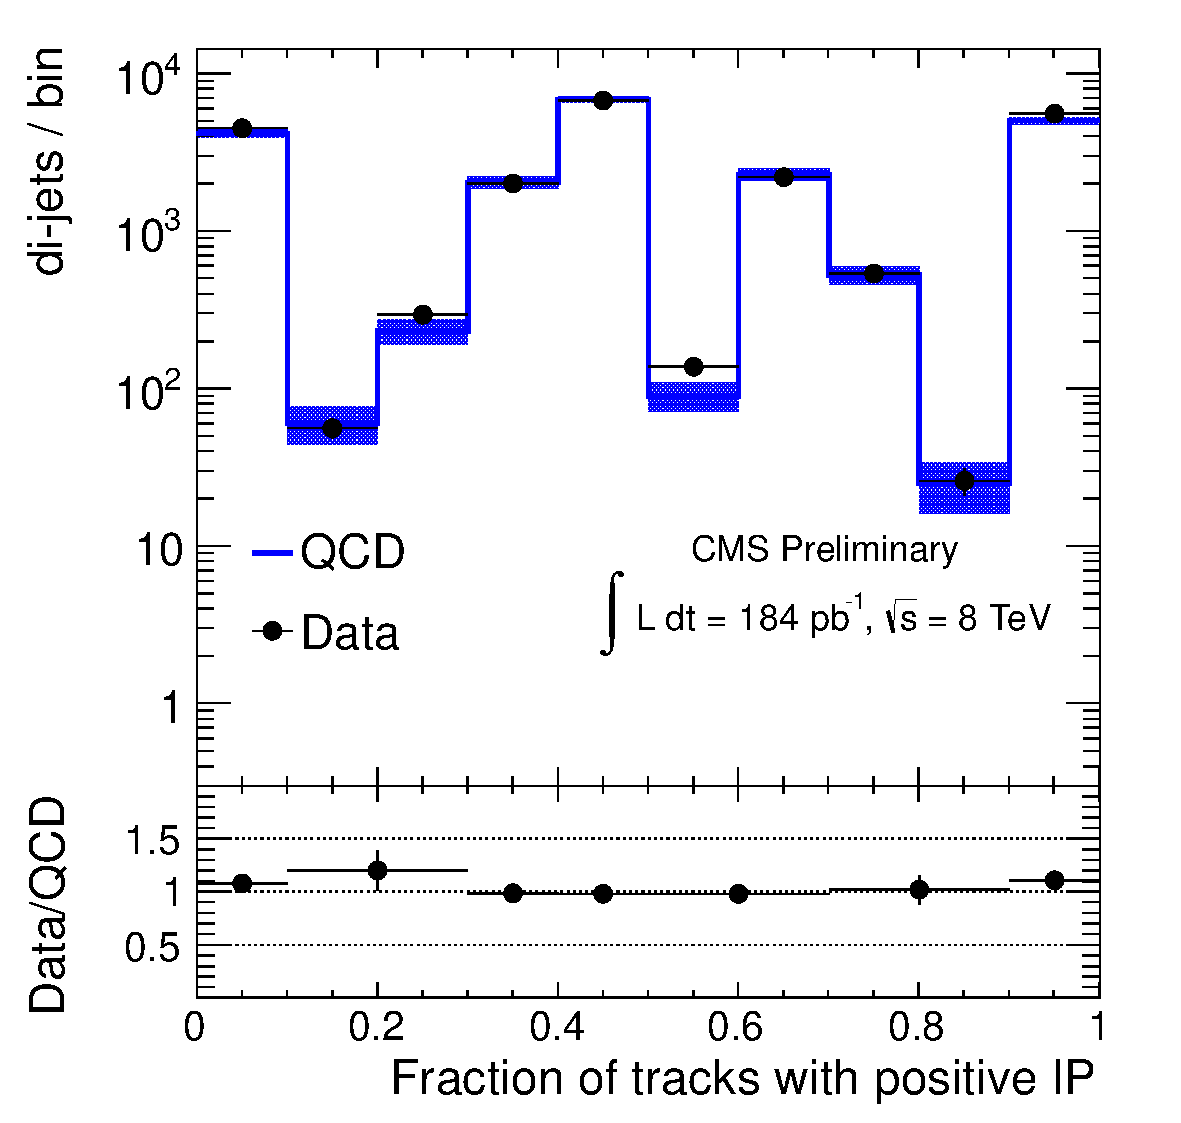
\includegraphics[width=0.49\textwidth]{plots/control/ctrl_Posip2dFrac.pdf}

\caption{Vertex variables. \label{fig:vertex}}
\end{figure}


\begin{figure}[htbp]
\centering
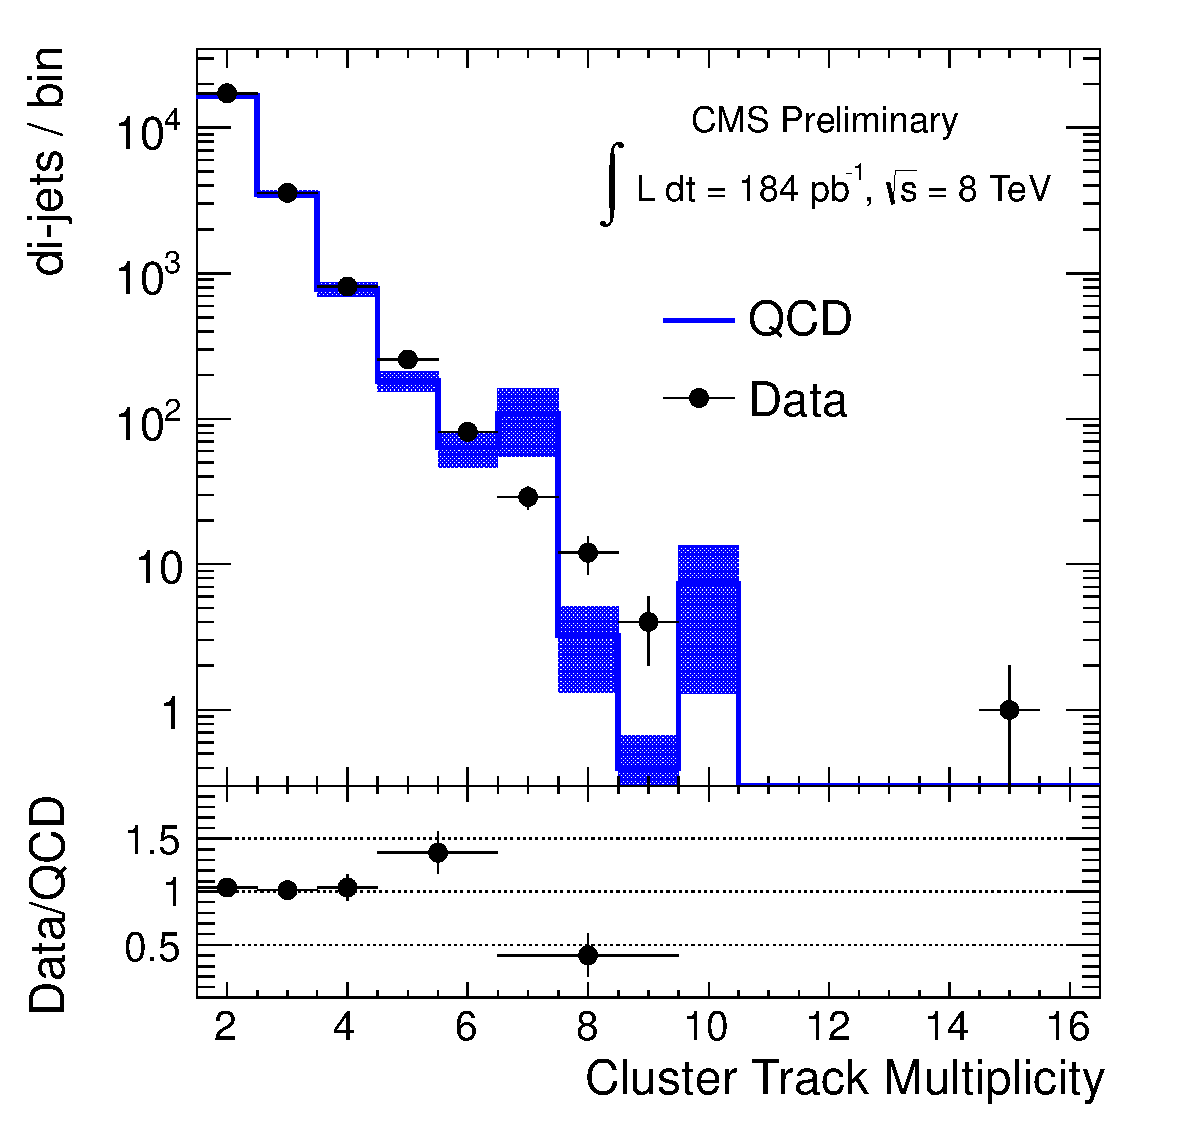
\includegraphics[width=0.49\textwidth]{plots/control/ctrl_clrN.pdf}
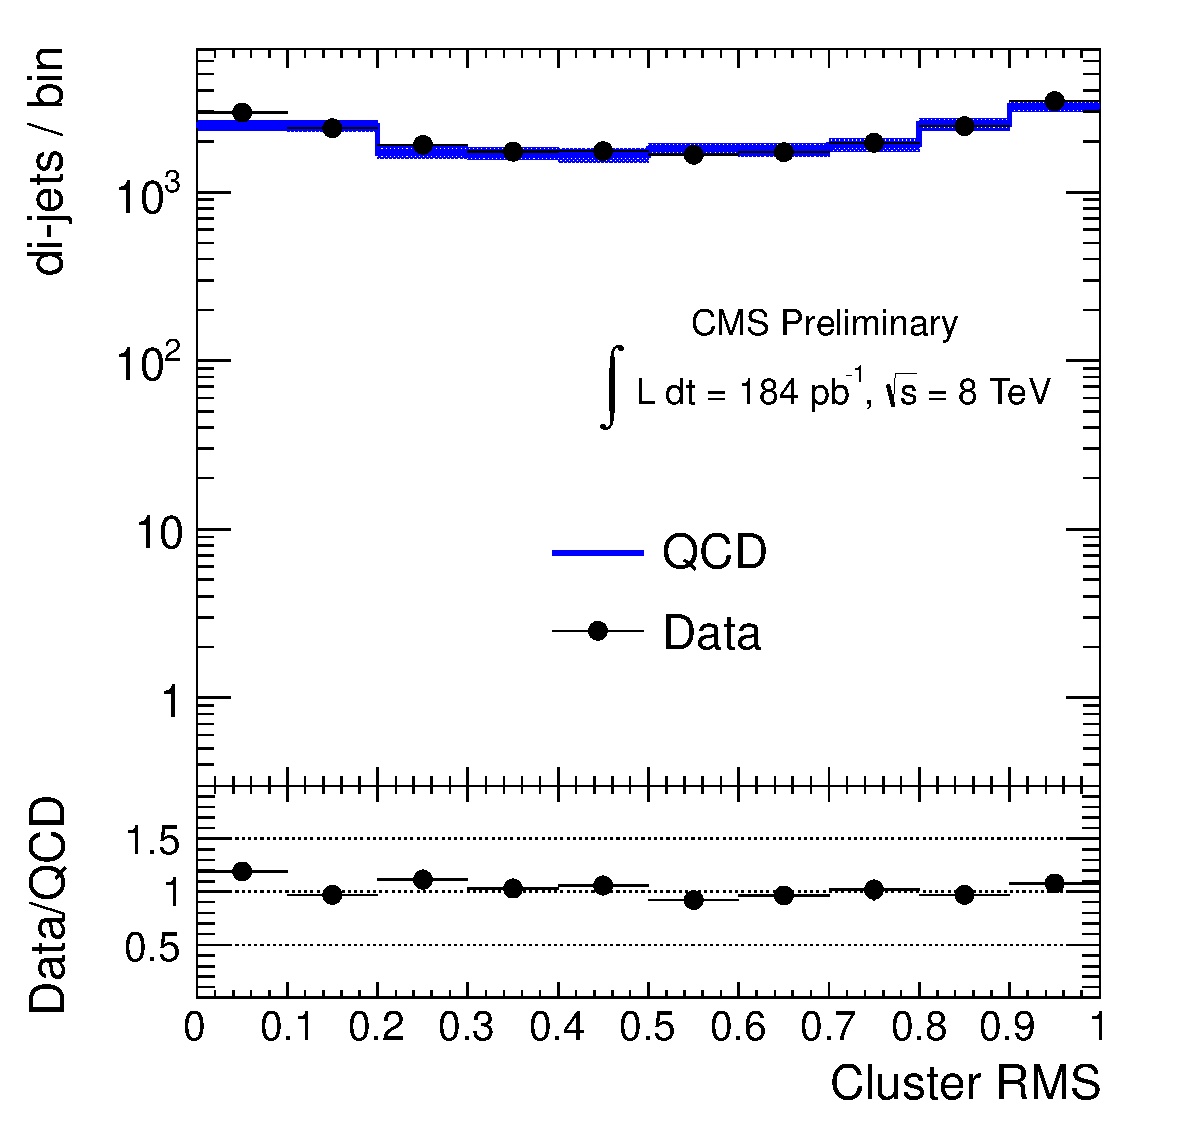
\includegraphics[width=0.49\textwidth]{plots/control/ctrl_clrRMS.pdf}

\caption{Cluster of $L_{xy}^{exp}$ variables. Candidates for which cluster RMS is above 1 do not share
tracks between the vertex and cluster reconstructions. \label{fig:cluster}}
\end{figure}

 

\chapter{Background}
This chapter focuses on a precise estimate of the search background. The
background prediction is of crucial importance for searches beyond the SM, because an observation
of an upward deviation with respect to the background prediction may hint at a new discovery.
First a data-driven background estimate is introduced. The benefit of a data-driven technique
as compared to a simulation-based estimate is that it avoids possible issues of 
mismodelling. Then tests of the background estimate are performed 
in control regions to establish the correctness of the method and to assess
its systematic uncertainty.


\section{Method of uncorrelated variables (ABCD)}


% We use an extension of the ABCD method 
% a little paragraph in there saying something like: to establish the notation, we consider a simple version of the ABCD method
% involving two independent cuts. 

% make an introduction about the ABCD method for only two variables

\label{sec:abcd}
We use a data-driven method of independent selections, ``the ABCD method".
To establish the notation, we introduce a simple version of the method that involves two 
independent selection criteria. As schematically presented in Fig.~\ref{fig:abcd} 
with two selection criteria one can divide the events into four
regions.
\begin{figure}[htbp]
\centering
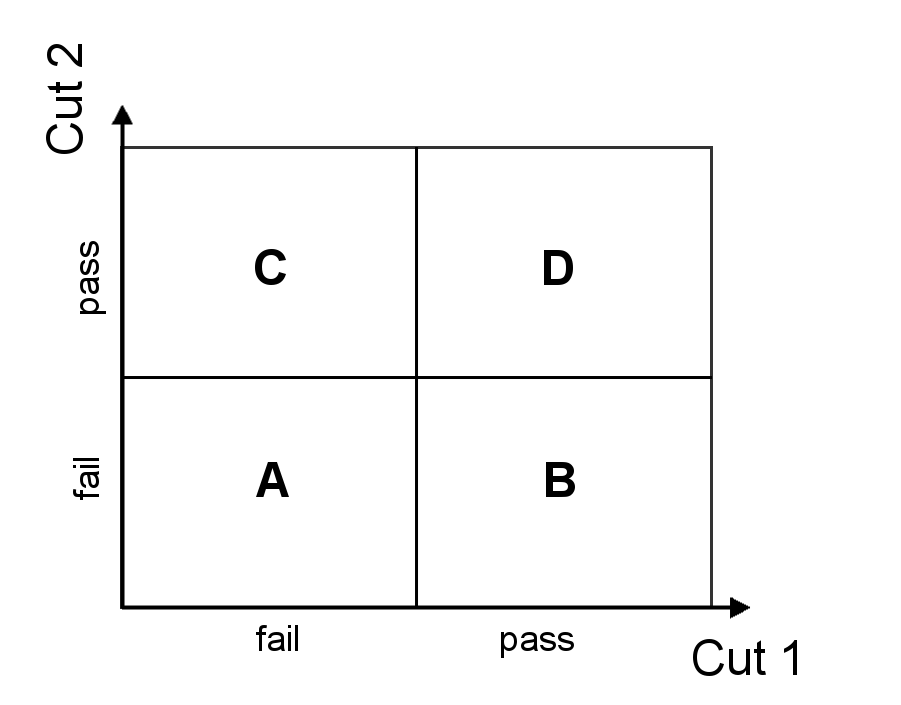
\includegraphics[width=0.65\textwidth]{plots/abcd.png}
\caption{Naming convention for the regions used in ``the ABCD method".\label{fig:abcd}}
\end{figure}
The regions A, B, and C are background dominated because the events that fall into those regions fail at least 
one of the selection criteria which have been optimized for signal detection. 
Given that for background events the probability of passing the first criterion is independent 
from whether it passes the second criterion, the number
of background events in the signal region, D, can be obtained from the event counts in regions A, B and C using the formula:

\begin{equation}
\text{D} = \frac {\text{BC}}{\text{A}}
\end{equation}


In this analysis, we use an extension of ``the ABCD method" using
 three, instead of two, independent selection criteria, see Section \ref{sec:selection} for the definitions of those criteria for displaced dijets. 
The three selection criteria divide the events into eight
regions (A, B, C, ..., H), as listed in Table \ref{tab:regions}, with  H being the signal region.

\begin{table}[htbp]
\centering
\caption{Naming convention for the regions used in background estimation. "+" corresponds to a selection 
being applied, while "--" to a selection being inverted. \label{tab:regions}}
\vspace{0.1cm}
\begin{tabular}{cccc}
 \hline
  Region & selection 1 & selection 2 & selection 3 \\
 \hline
 A & -- & -- & -- \\
 B & + & -- & -- \\
 C & -- & + & -- \\
 D & -- & -- & + \\
 E & -- & + & + \\
 F & + & -- & + \\
 G & + & + & -- \\
 H & + & + & + \\
\hline
\end{tabular} 
\end{table}

With three independent selections the background level in the signal region H can be estimated from various combinations
of the event counts in other regions. Among the suitable combinations 
there are six that use event counts in only
three regions, namely:
\begin{enumerate}
 \item FG/B = (+,--,+)(+,+,--) / (+,--,--) -- the right hand side of the equation uses
 a notation that indicates which selections are passed and which are failed by 
 the events in a given region
 \ie (+,--,+) corresponds to region F where events pass the first and third selection,
 while they fail the second selection;
 \item EG/C = (--,+,+)(+,+,--) / (--,+,--)
 \item EF/D = (--,+,+)(+,--,+) / (--,--,+)
 \item DG/A = (--,--,+)(+,+,--) / (--,--,--)
 \item BE/A = (+,--,--)(--,+,+) / (--,--,--)
 \item CF/A = (--,+,--)(+,--,+) / (--,--,--)
\end{enumerate}


%\begin{itemize}
%\item FG/B, EG/C, EF/D - for these background estimates the numerator regions are such that two selections
%are applied and one is inverted, while the denominators are regions where one selection
%is applied and two are inverted;
%\item DG/A, BE/A, CF/A - the numerators are such that the two regions taken together involve
%all three selections both applied and inverted

%for these background estimates two selections are combined into one
%and therefore we apply and inverted
%these choices combine two selections together and apply or invert it with the 
%remaining selection.
%\end{itemize}

A seventh background prediction can be formed by combining three of the predictions above:

\begin{equation}
\frac{\text{DG/A}\cdot\text{BE/A}}{\text{EG/C}} = \frac{\text{BCD}}{\text{A}^2} = \frac{(+,-,-)(-,+,-)(-,-,+)}{(-,-,-)^2}
\end{equation}


The combination BCD/A$^2$ is constructed from regions with at least two selections inverted.
It minimizes the statistical uncertainty on the background estimate, because in regions 
A, B, C, and D
the background event counts are largest. We use BCD/A$^2$ as our background prediction
central value.
%A seventh background prediction, which minimizes statistical uncertainty,
%can be formed by combining three of the estimates above:
%\begin{equation}
%DG/A * BE/A / EG/C = BCD/A^2
%\end{equation}
In the case of perfectly independent 
variables, all above combinations predict statistically consistent  amounts of background. 
However, to account for possible systematic
effects due to residual dependence of the selections, we assign a systematic uncertainty 
that is equal to the largest difference 
between BCD/A$^2$ and any of the six other predictions.

\section{Selection optimisation}
\label{sec:cutvalues}
We determine the numerical values of the selection criteria that are employed in the background estimation procedure 
by optimizing the expected limit for each tested signal model.
The signal models considered include various values of the \Higgs mass, the \X mass, and the \X lifetime.
The selection variables
do not strongly depend on the particles masses, therefore the optimal selection criteria
vary only as a function of the
mean transverse decay length ($L_{xy}$)
of the \X bosons. We use two sets of selection criteria,
depending on whether the mean
$L_{xy}$ of the \X bosons is below or above 30\cm. The selection criteria are
detailed in Table \ref{tab:background}.

\begin{table}[htbp]
\centering
\caption{Optimised selection criteria and the corresponding background expectations with their statistical and systematic uncertainties.\label{tab:background}}
\vspace{0.1cm}
\begin{tabular}{r|c|c}
%\hline
$\bf L_{xy}$ \bf selection &\bf  $\bf <30\cm (low)$ & \bf  $\bf >30\cm (high)$ \\
\hline
prompt tracks & $\leq1$ & $\leq1$ \\
%\hline
prompt energy & $<0.15\%$ & $<0.09\%$ \\
%\hline
vertex/cluster disc. & $>0.9$ & $>0.8$  \\
\hline
\bf expected bkg. & $\bf 1.60\pm0.26(stat)\pm0.51(syst)$ & $\bf 1.14\pm0.15(stat)\pm0.52(syst)$ \\
%\hline
\end{tabular}
\end{table}

\section{Background tests}
\label{sec:backgroundtests}
The background estimation procedure described in Section \ref{sec:abcd} is general and can be applied
to any dataset if the selections used are independent.
In this Section we describe various background closure tests
 performed in QCD MC simulation and 
selected control regions in data.
We test the optimal selection criteria from Section \ref{sec:cutvalues} and also other various selections points.
%In order to perform background tests we apply various selections, not only the optimal ones
%listed in Section \ref{sec:cutvalues}.
The figures shown in the following Sections present the observed number
of events along with the seven background estimates which were described
 in Section \ref{sec:abcd}.
Uncertainties are statistical only. 
For each of the tested selection points the background prediction 
and its uncertainty are obtained 
using the prescription from Section \ref{sec:abcd}. 
%The background prediction and its statistical 
%and systematic uncertainties are
% not explicitly plotted given that all of the 7 combinations employed in its derivation are shown.  
The compatibility between the predicted and observed background is estimated with a {\it p-value} for each measurement. 
%The {\it p-values} are then converted into {\it significances} using the normal distribution. 
 The {\it p-value}
is computed with respect to the estimated background probability density function (p.d.f.). 
The background prediction has an associated uncertainty, 
therefore the background p.d.f. is a Poissonian function convolved  
with a Gaussian error function. The probability of observing $n$ background events is given by:
\begin{equation}
B(n,b,\sigma_b)= \frac{1}{\sqrt{2\pi}\sigma_b} \int_{0}^{\infty} 
\exp\left[ -\frac{\left(x-b\right)^2}{2\sigma_b^2}\right]\frac{x^n e^{-x}}{n!}dx
\label{eqn:bdensity}
\end{equation}
where $b$ is the background central value and $\sigma_b$ is the total uncertainty.
The Gaussian probability density of the background mean has been truncated at 
0 in order to avoid unphysical values. Such a truncation results in a not properly normalized p.d.f. in Eq. 
\ref{eqn:bdensity}, however the {\it p-values} computed according to Eq. \ref{eqn:pvalues} take the 
normalization into account.   
\begin{equation}
{\it p} (n_\text{obs},b,\sigma_b) = \sum_{k\geq n_{obs}} B(k,b,\sigma_b) / \sum_{k} B(k,b,\sigma_b)
\label{eqn:pvalues}
\end{equation}
The {\it p-values} are then converted into {\it significances} using the normal
 distribution. The {\it significances} are shown in the bottom plots (Figs. 
\ref{fig:bkg_MC}-\ref{fig:10percent}) aligned to the corresponding background
measurements.  

\subsection{QCD MC background prediction}
\label{subsec:bkgQCDMC}

Due to the limited statistics of the QCD MC samples, the displaced jet trigger requirement has been removed. In addition, the background is estimated with looser
 selection on prompt tracks variables compared to the final selection. 
In order to validate the background prediction with 
the observed Poissonian event counts, the cross-section weights (Table \ref{tab:backgrMC}) 
are removed. 
Therefore this test serves only to identify biases due to non-independent selections,
and cannot be translated
into a background prediction in data.  
As shown in Fig. \ref{fig:bkg_MC} good agreement between predicted and observed background level is found, 
and the discrepancy is not significant for the tested selection points. Therefore, we conclude that the  
bias due to possible interdependence between the variables is small in the QCD MC samples. 

\begin{figure}[htbp]
  \centering
  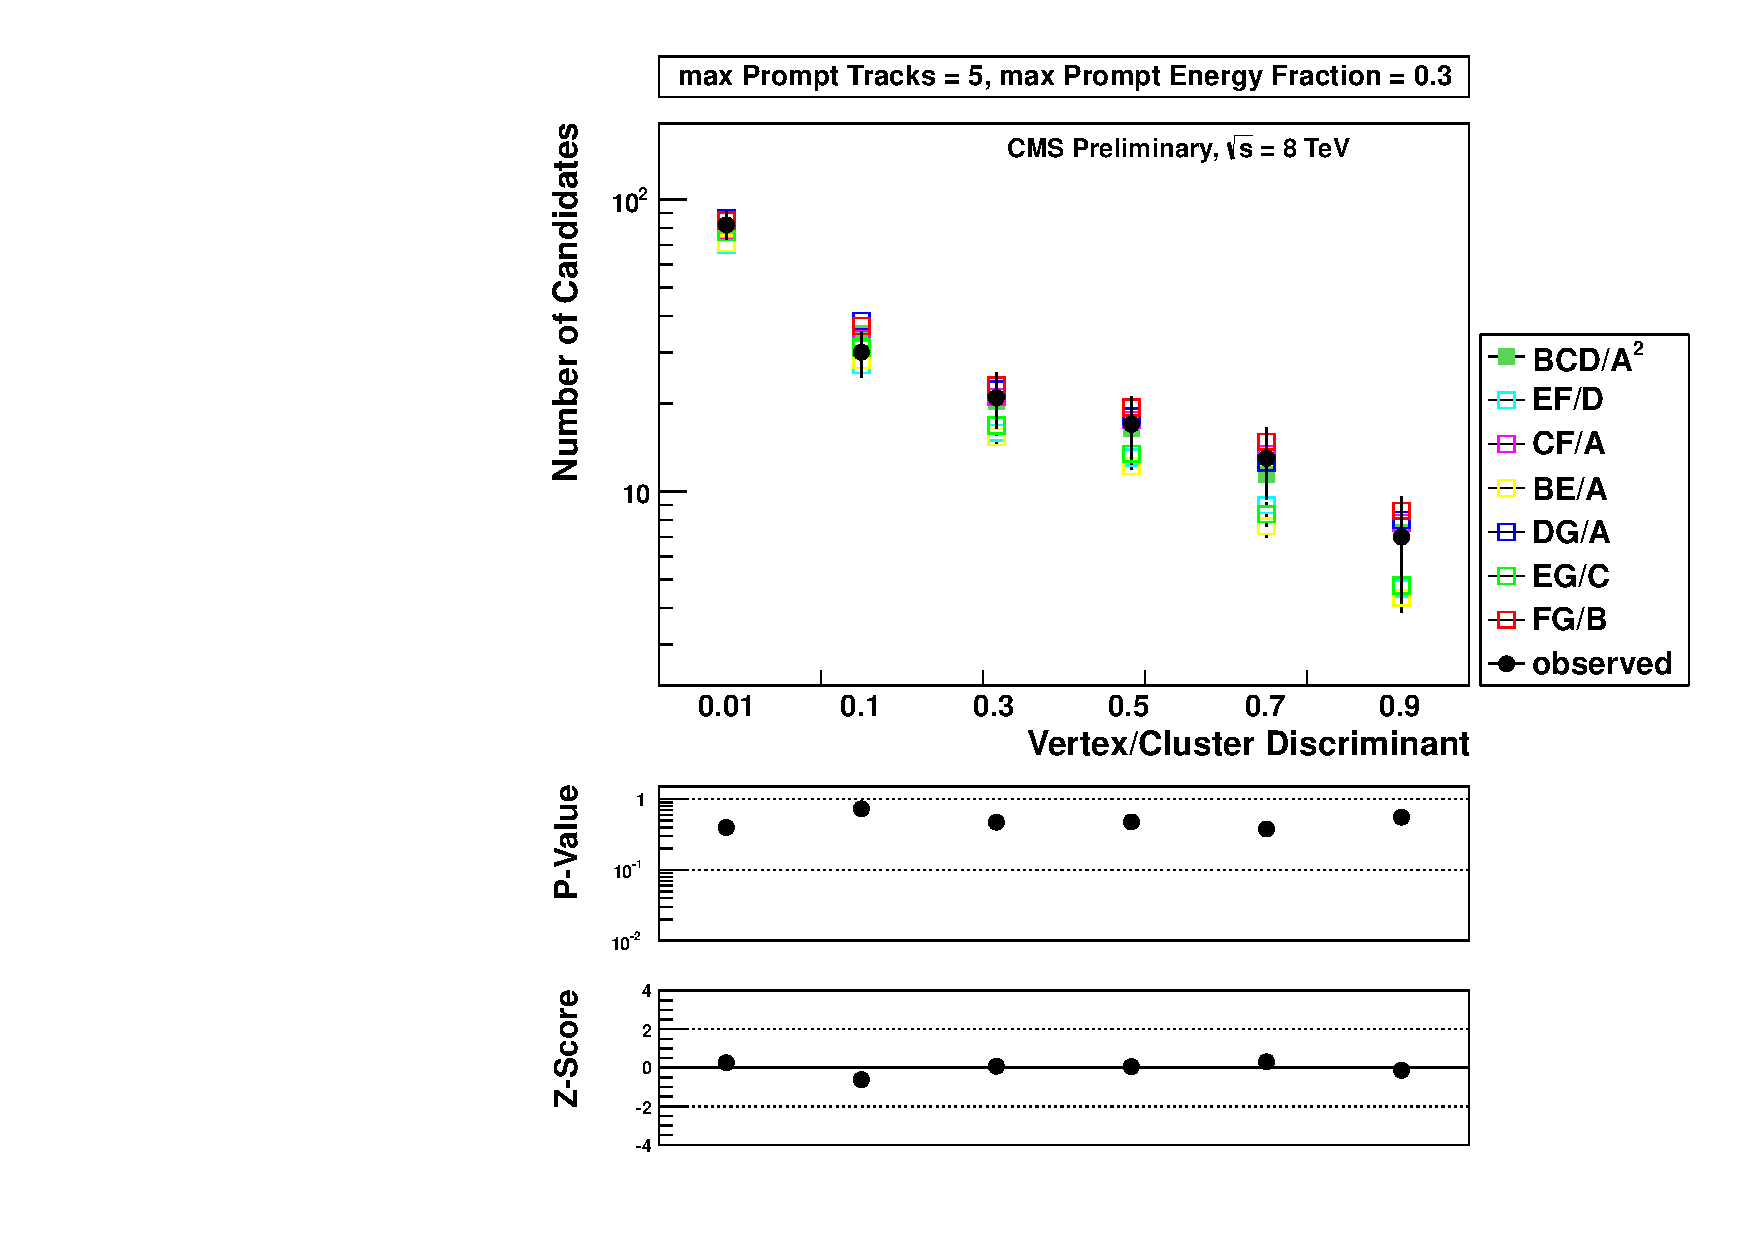
\includegraphics[width=0.495\textwidth]{plots/background/bkg_MC1.pdf}
  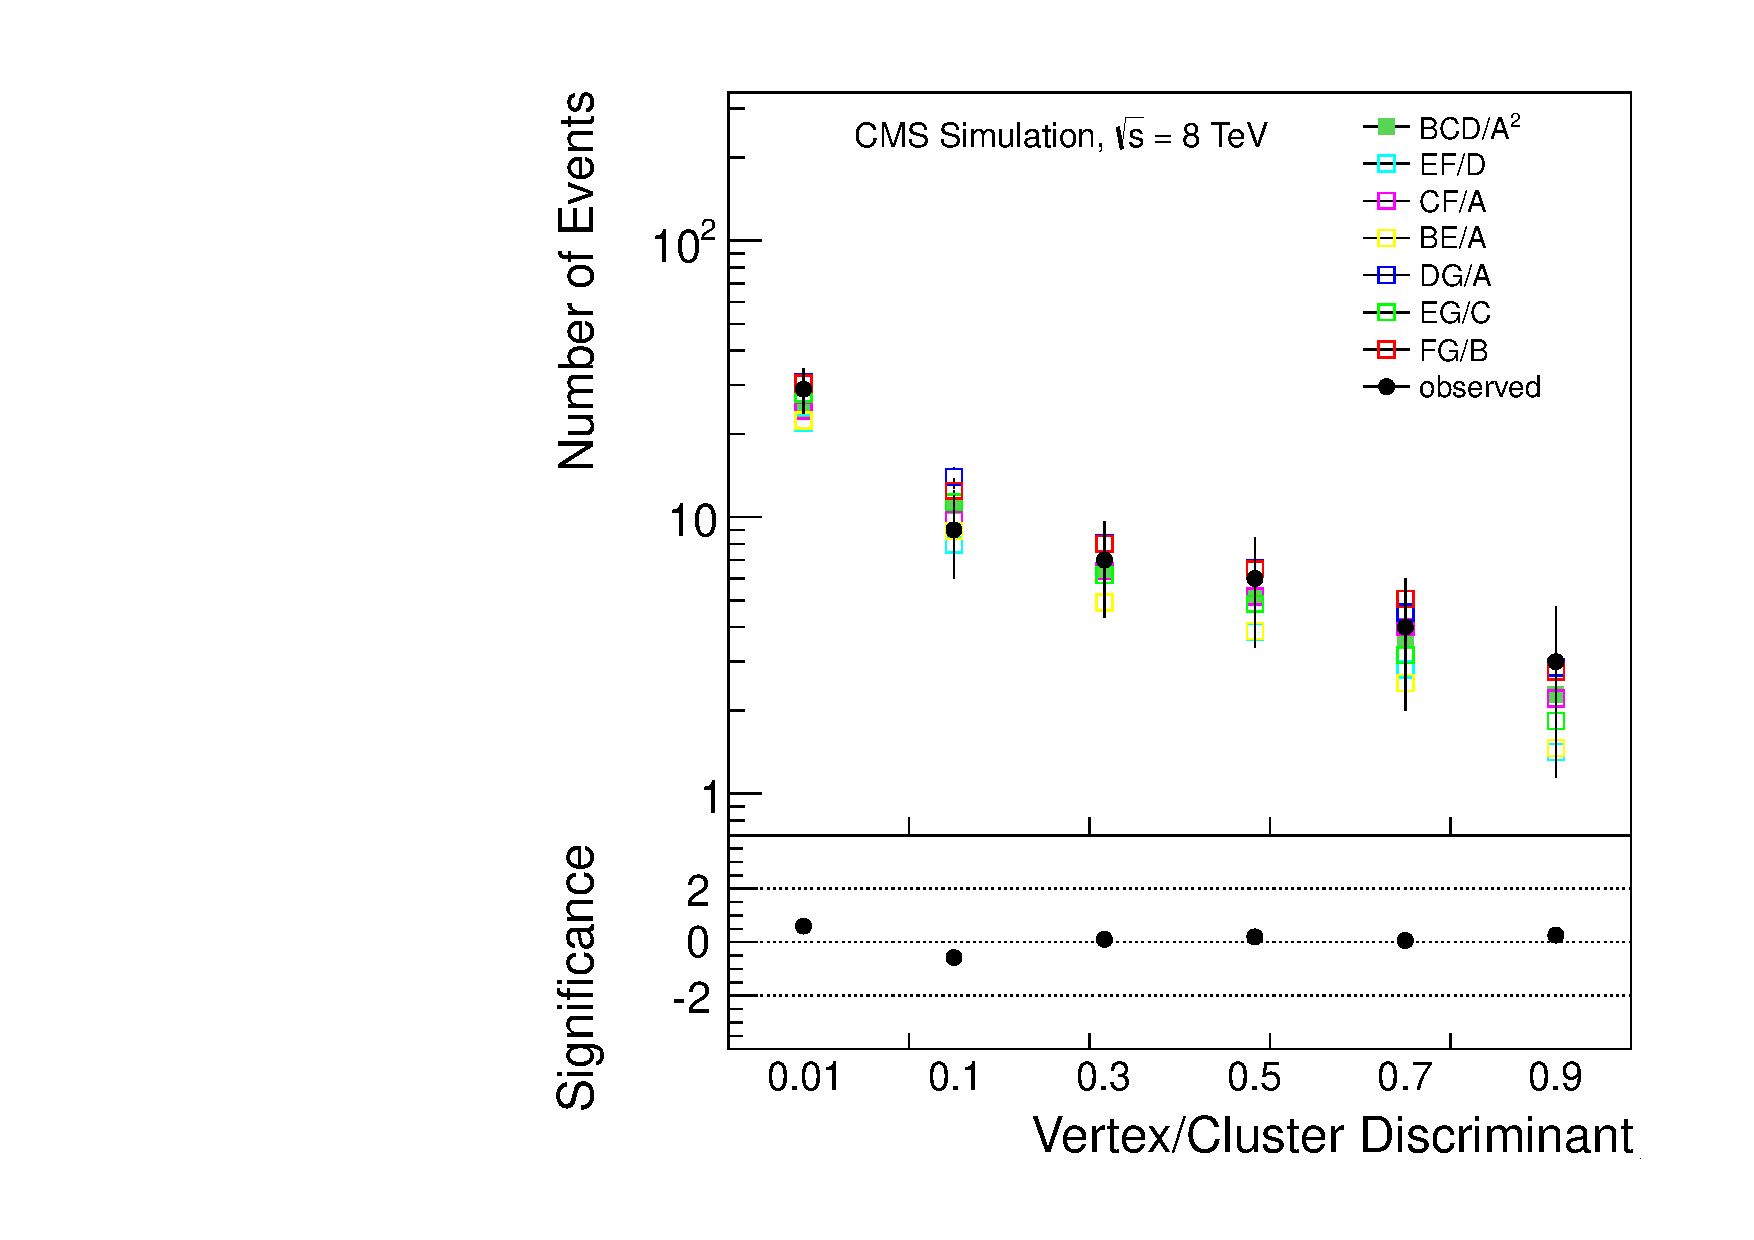
\includegraphics[width=0.495\textwidth]{plots/background/bkg_MC2.pdf}
  \caption{Predicted and observed background level for QCD MC sample as a function of the vertex discriminant selection criteria.
The selection requires at most 5 (left) and 4 (right)  prompt tracks and that their jet energy fraction be below 30\% (left) and 25\% (right), which
is significantly looser than the final selection. \label{fig:bkg_MC}}
  \end{figure}


\subsection{Data control region}
\label{subsec:bkgCtrl}

As a data control region we use candidates passing all of the preselection criteria listed in Section
 \ref{sec:selection}, but with the {\it missing hits} selection inverted. We again choose only 
 one candidate per event applying the same procedure as described in Section \ref{sec:selection}.
 Such a region has a very small 
signal acceptance compared to the signal region, as the {\it missing hits} criterion has a very high signal 
efficiency, while providing a
background sample with good statistics. Using this control region we are able to test final selection
criteria with amounts and uncertainties of predicted background comparable to the signal region. 
 As shown in Fig. \ref{fig:bkg_NMiss}, 
the background predictions in this control region are in good agreement 
with the observed background levels. Given that the significance
of the discrepancies is small, we conclude
that the background estimation method is valid and the systematic uncertainty on the background
 prediction is not underestimated.

\begin{figure}[htbp]
\centering
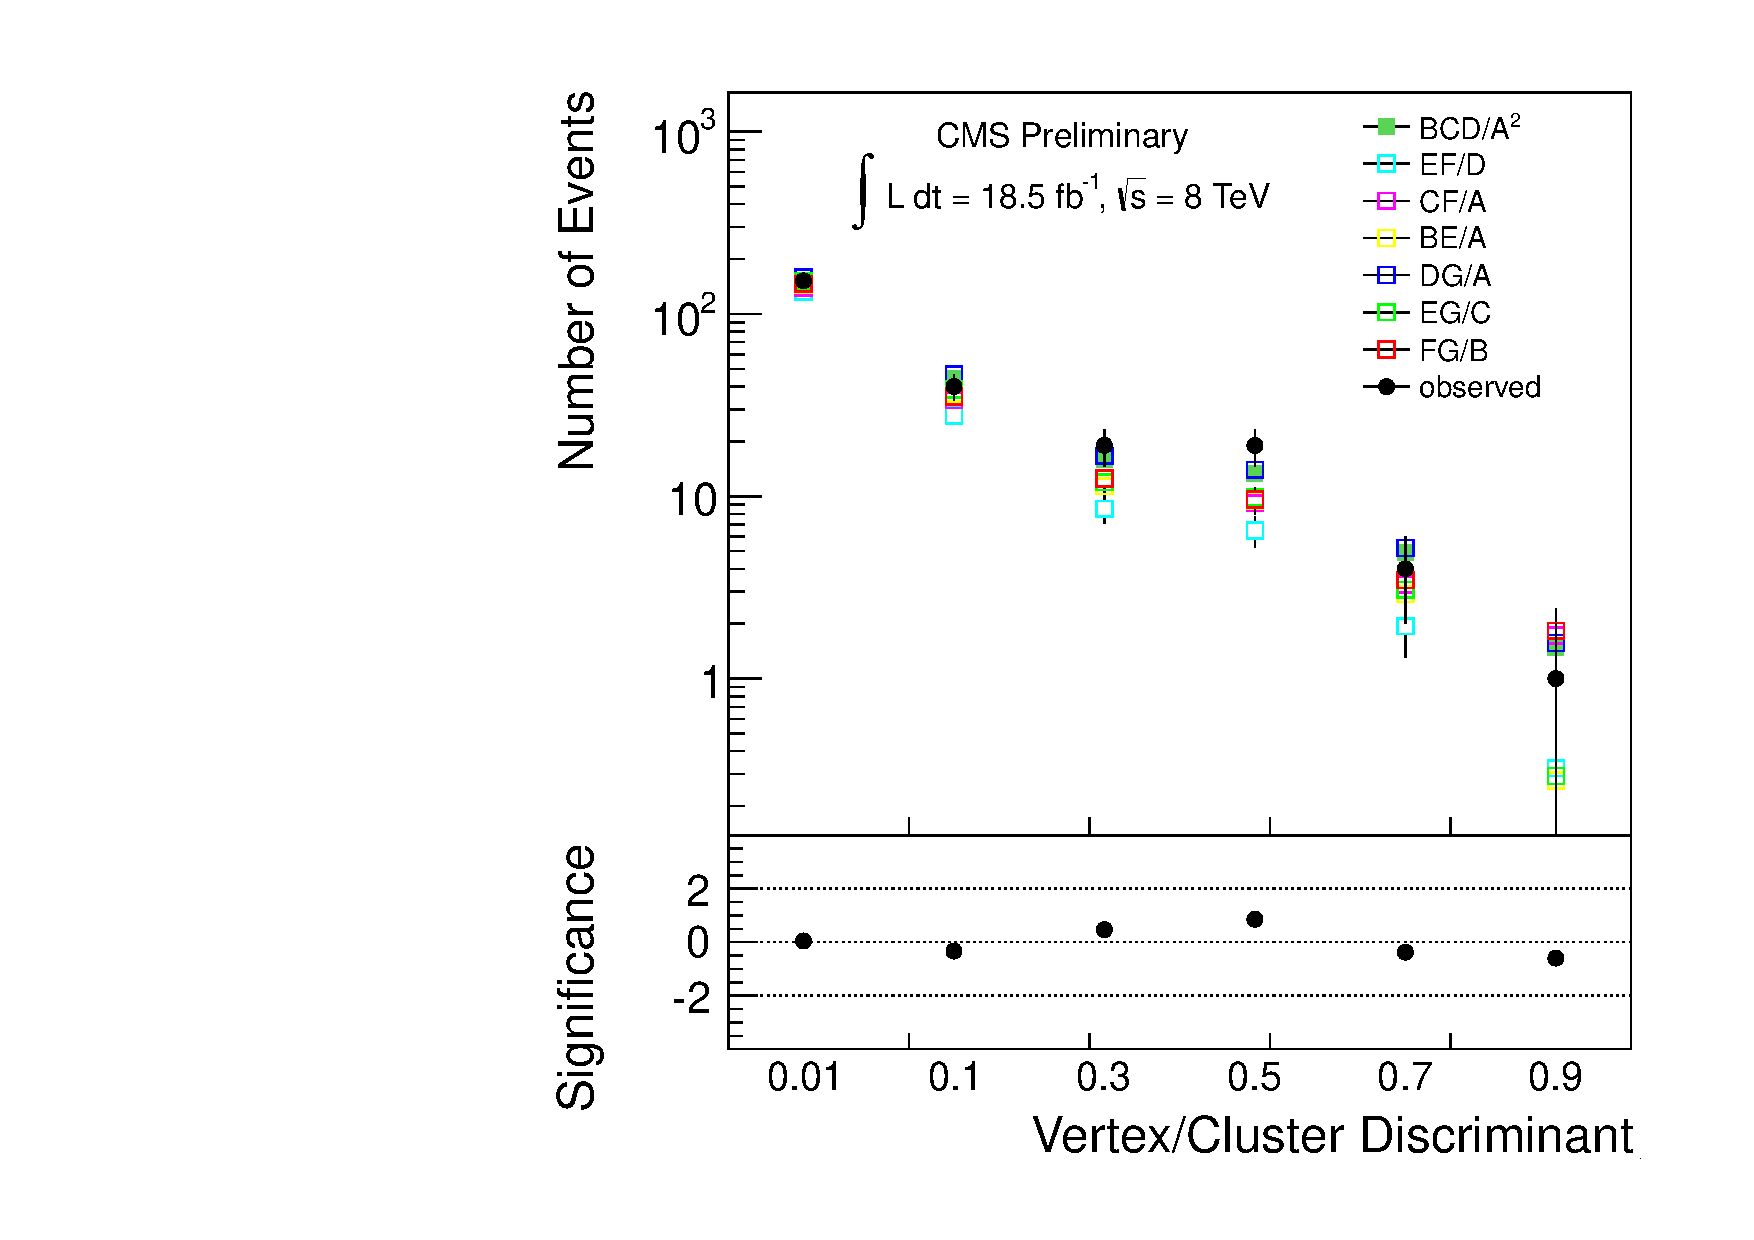
\includegraphics[width=0.495\textwidth]{plots/background/bkg_NMiss1.pdf}
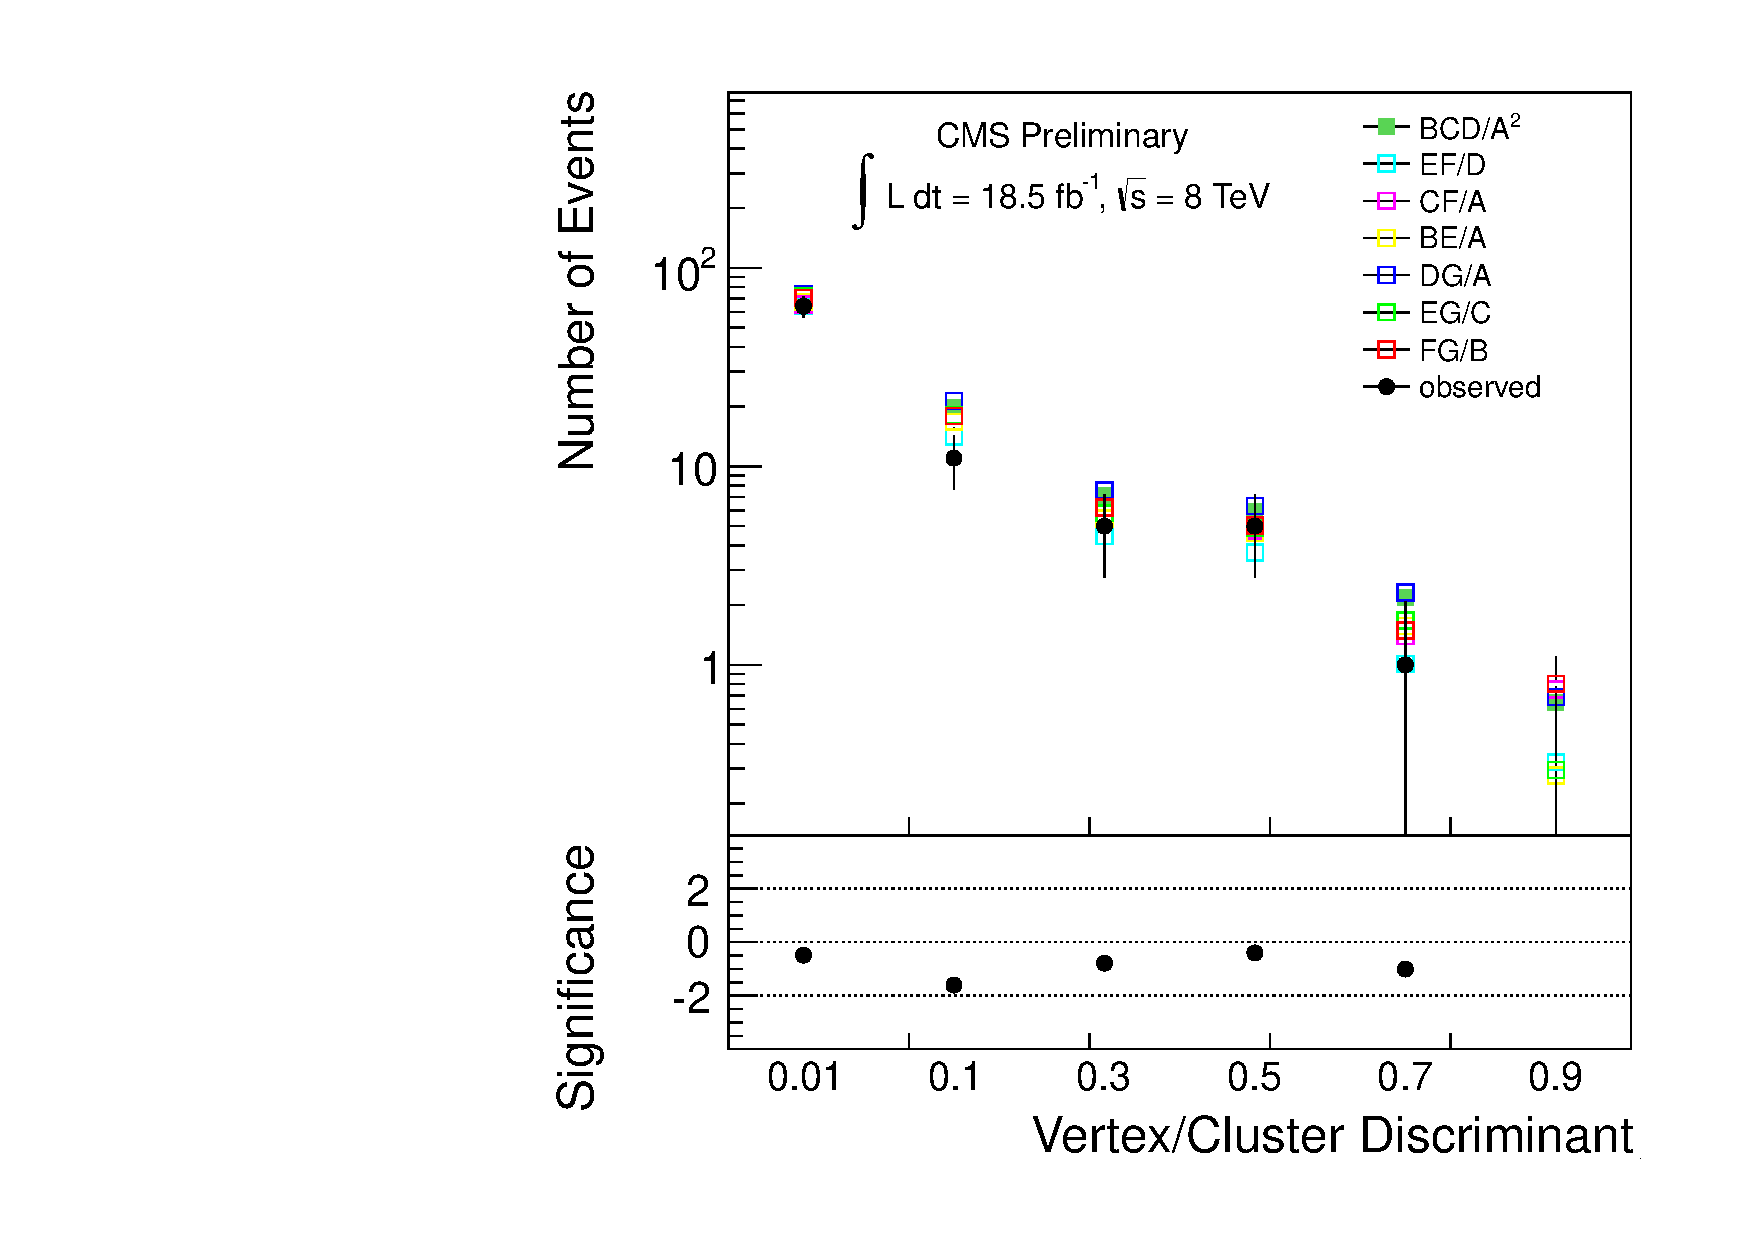
\includegraphics[width=0.495\textwidth]{plots/background/bkg_NMiss2.pdf}
\caption{Predicted and observed background levels in the data control region as a function of the vertex
discriminant selection criteria. The selection requires at most 1 prompt track and that the jet energy fraction carried by prompt tracks is
below 15\% and 9\% on the left and right plot, respectively.\label{fig:bkg_NMiss}}
\end{figure}

\section{Background estimate based on 10\% of the dataset}
\label{sec:partunblinding}

In order to check that there is no anomalous background present,
 we initially examined the data corresponding to only 10\% of all available 
data in the signal region.  
We select the data using one out of every ten luminosity sections, where a luminosity
section is a period of approximately 23 seconds of active data taking. This way of choosing the data is sensitive to possible problems that occur only for selected data taking periods, and also to effects that may arise from
correlations between consecutive events accepted by the trigger. A comparison of the data and predicted
background is presented in Fig. \ref{fig:10percent}. No anomalous background is observed in this sample,
however, the background predictions are small, thus limiting the statistical
power of the test.

\begin{figure}[htbp]
  \centering
  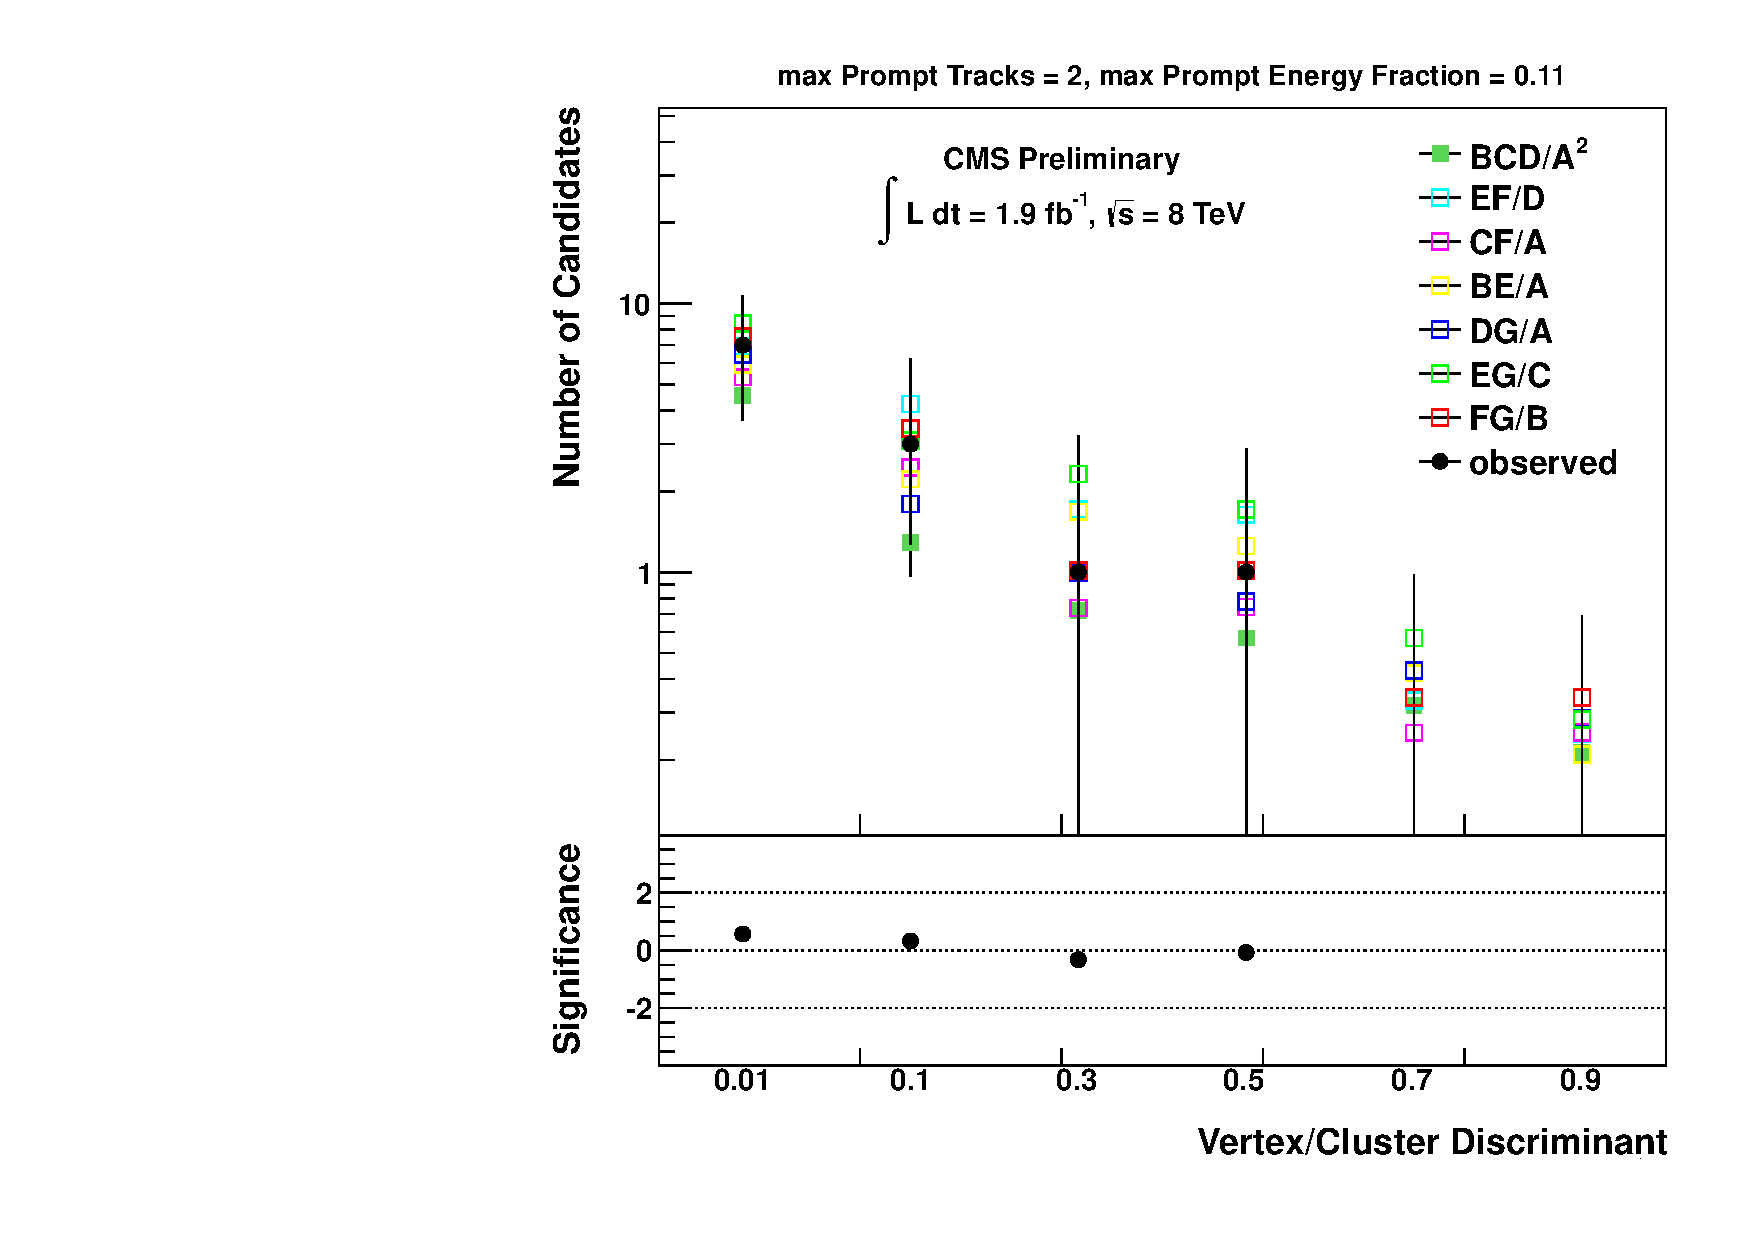
\includegraphics[width=0.495\textwidth]{plots/background/tenpercent1.pdf}
  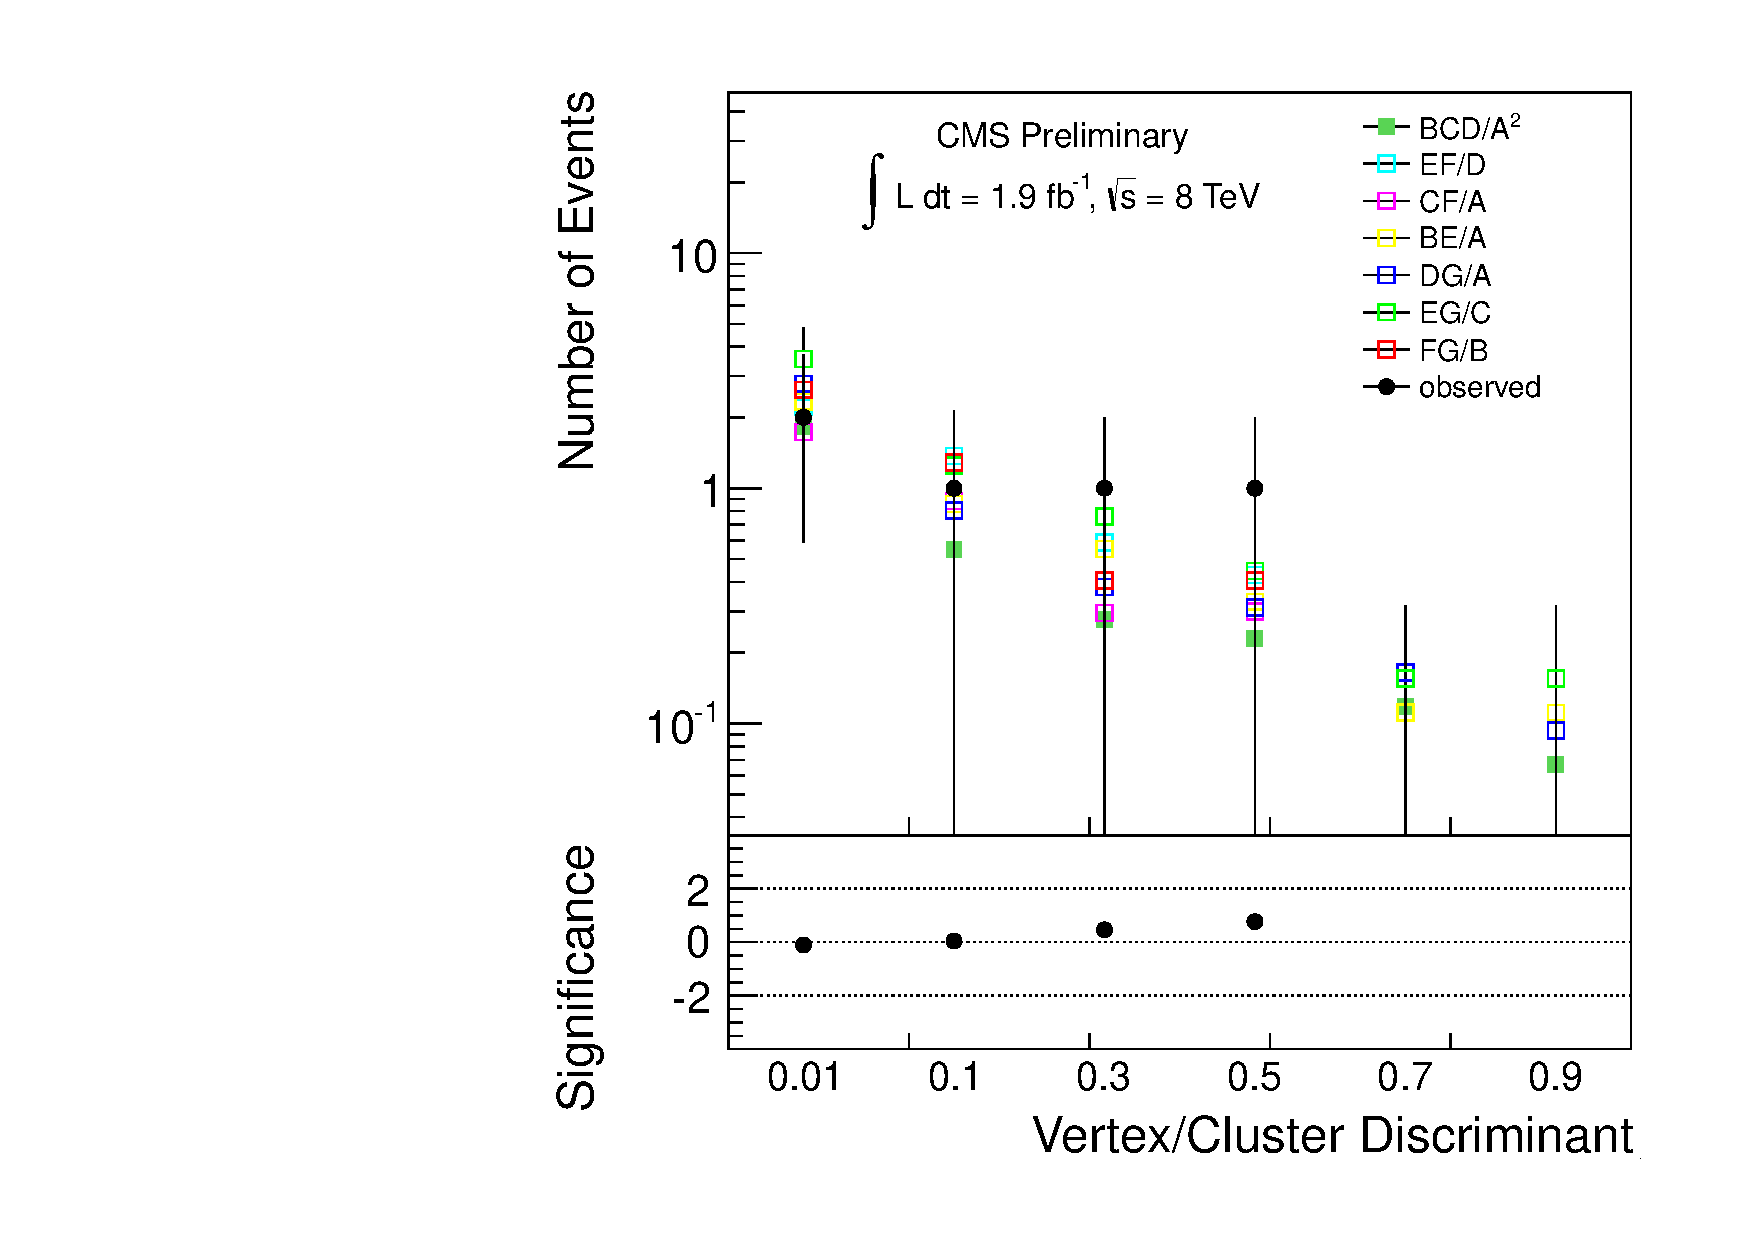
\includegraphics[width=0.495\textwidth]{plots/background/tenpercent2.pdf}
  \caption{Data and predicted background level in the 10\% data sample as a function of vertex discriminant
selection criteria. The selection requires at most 2 (left) or 1 (right) prompt tracks while the jet energy 
fraction carried by the prompt tracks is required to be less than 11\%. \label{fig:10percent}}
\end{figure}  




\chapter{Systematic Uncertainties}
We describe the sources of systematic uncertainty which inlcude those related to 
the background prediction, the integrated luminosity, and the signal reconstruction efficiency. 
The signal efficiencies are obtained from Monte Carlo simulations of the various signals processed
through full detector simulation. The systematic uncertainties are then estimated by determining
the relevant differences between data and simulation using control samples. The sources
of systematic uncertainty are discussed below and their impact on the analysis result is
evaluated.
 
As discussed in Section \ref{sec:cutvalues} the analysis aims to optimize the expected limit
in case no signal is present in the data.
 With the level of the predicted
background, we study the impact of a hypothetical signal efficiency systematic uncertainty 
on the limit result in Appendix \ref{app:sys}. 
Upon an increase in signal systematic uncertainty the expected limit degrades relatively slowly,
therefore when evaluating MC related systematic effects we take a conservative approach.

\section{Background}
The systematic uncertainty on the estimated background differs depending on the final selection
 as listed in Table \ref{tab:background}. The relative systematic uncertainty is estimated using the prescription
described in Section \ref{sec:abcd}. It is evaluated to be 32\% and 46\%
for {\it low} and {\it high} $L_{xy}$ selections with 1.60 and 1.14 predicted background candidates respectively. 
The 7 background predictions from which the systematic uncertainty is derived are listed in Table \ref{tab:sigbkg}.

\begin{table}[htbp]
\centering
\caption{Predicted background level for the final selections obtained with 7 combinations using the
method of independent selections. \label{tab:sigbkg}}

\begin{tabular}{lcc}

\hline
Selection & {\it low} $L_{xy} $& {\it high} $L_{xy}$ \\
\hline
$BCD/A^2$ & 1.60 & 1.14 \\
$FG/B$ & 1.21 & 1.00 \\
$EG/C$ & 1.92 & 0.84 \\
$DG/A$ & 1.76 & 1.25 \\
$BE/A$ & 1.72 & 0.77 \\
$CF/A$ & 1.08 & 0.92 \\
$EF/D$ & 1.16 & 0.62 \\
\hline

\end{tabular}
\end{table} 


\section{Luminosity}
For the running period corresponding to this analysis, CMS estimates the relative uncertainty on the luminosity to be 4.4\% \cite{CMS-PAS-LUM-12-001}.

\section{Effect of Pile-Up}
The likelihood of a given number of pile-up events occurring in the data can be calculated from the distribution
 of the instantaneous luminosity during the 2012 LHC run. The number of true pile-up events in the Monte Carlo
 simulation is also known. The simulation can therefore be re-weighted to match the data. 

The systematic uncertainty in this procedure is estimated by adjusting the re-weighting, so as to account
 for uncertainties related to pile-up modeling. 
The effect of a $\pm$5\% variation in the number of interactions is estimated and gives rise 
to a relative systematic uncertainty in the signal reconstruction efficiency 
of less than 2\% for all mass and lifetime points considered. The signal reconstruction efficiency as
a function of number of primary pile-up vertices is shown in Figure \ref{fig:effPU}. No significant
decrease in efficiency is observed as the number of primary pile-up vertices increases.

\begin{figure}[htbp]
\centering
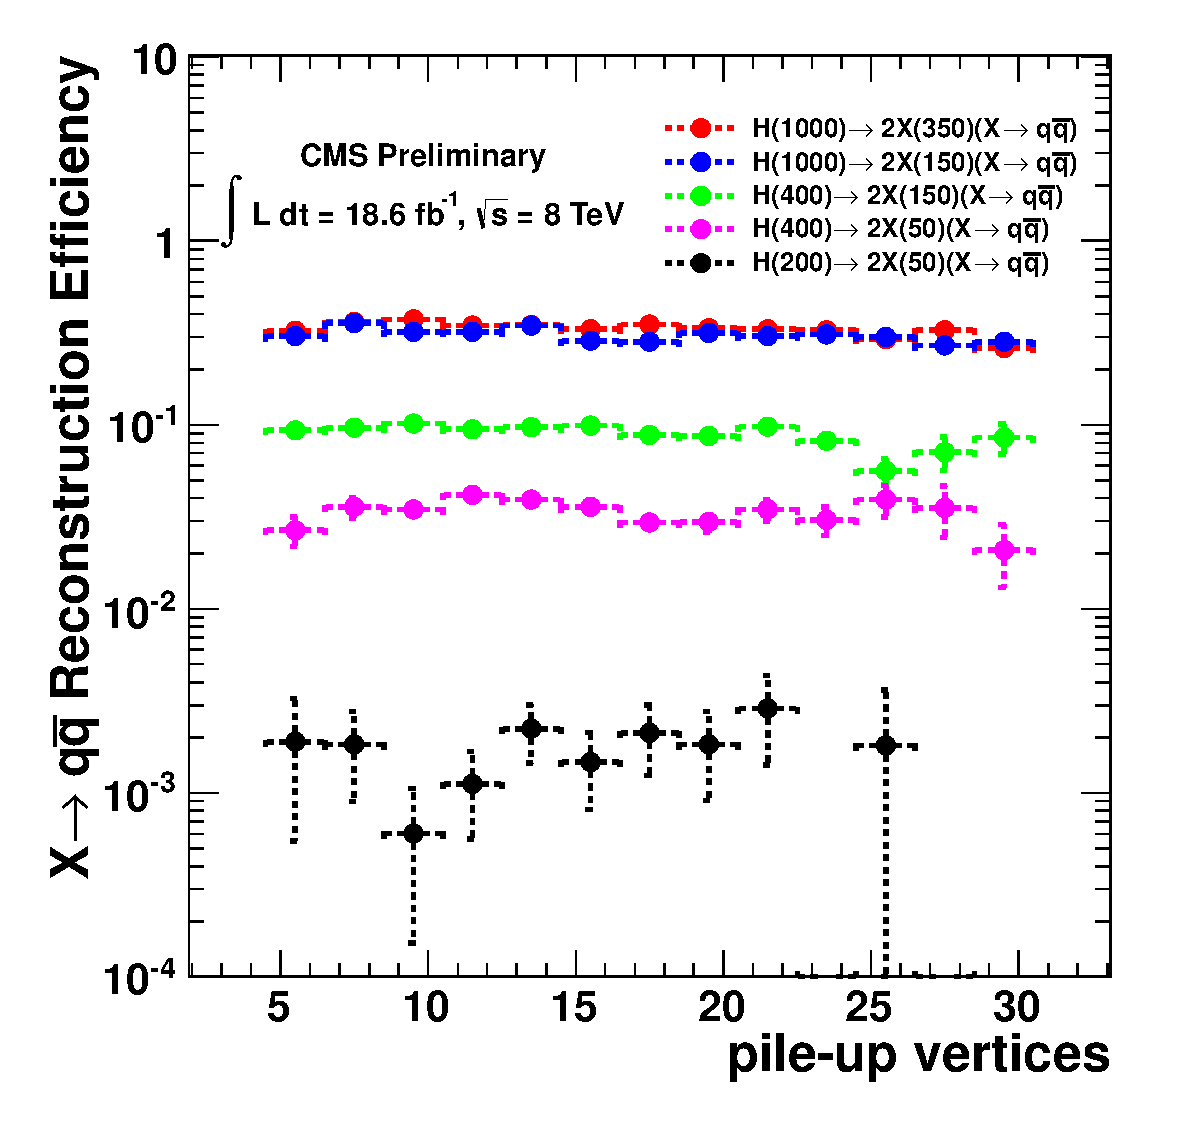
\includegraphics[width=0.49\textwidth]{plots/signal/effPU.pdf}
\caption{Reconstruction efficiency as a function of number of pile-up vertices for selected
signal models.\label{fig:effPU}}
\end{figure}

\section{Primary vertex selection}
\label{subsec:pv}
The relevant impact parameters and decay lengths are computed 
with respect to the primary vertex which has the highest
squared transverse momentum sum of the tracks. If a dijet candidate does not originate from this vertex the impact
parameters would be computed incorrectly. The size of the luminous region, where the primary vertices lie,
 is $\sim$5\cm in the longitudinal direction and $\sim$15$\mu m$ in both transverse directions. 
Therefore the effect of an incorrect primary vertex assignment significantly increases the 3-D impact parameters,
 while for
the transverse impact parameters the effect is small as the size of the luminous region is smaller than the 
primary vertex resolution (20$\mu m$).
In the displaced dijet selection criteria the 3-D impact parameters are used to compute 
the number of jet prompt tracks, while all other criteria employ
only the transverse impact parameters. 
 We study the background level and signal reconstruction efficiency where all
 the relevant impact parameters and
decay lengths are computed with respect to the second, instead of the first, primary vertex. In this scenario 
the selection of an incorrect primary vertex is greatly enhanced. The predicted and
observed background level are detailed in Table \ref{tab:wrongvtx}.

\begin{table}[htbp]
\centering
\caption{Predicted and observed background for the optimised selections for first and second highest squared transverse momentum sum primary vertex in the event. Uncertainties on the background level include both statistical
and systematic uncertainties. \label{tab:wrongvtx}}
\begin{tabular}{lcc}
\\
 & low $L_{xy}$ (1$^{st}$ PV) & low $L_{xy}$ (2$^{nd}$ PV) \\
\hline
predicted bkg. & $1.60\pm0.57$ & $1.67\pm0.75$ \\
observed bkg. & 2 & 2 \\
\hline
\\
 &  high $L_{xy}$ (1$^{st}$ PV) & high $L_{xy}$ (2$^{nd}$ PV)\\
\hline
predicted bkg. & $1.14\pm0.54$ & $1.17\pm0.66$ \\
observed bkg. & 1 & 1 \\
\hline
\end{tabular}
\end{table}

The predicted background level minimally increases if a wrong primary vertex is used, while the increase is small
with respect to the background level uncertainty. The signal reconstruction efficiency 
does not significantly change whether the first or second leading primary vertex is used.

\section{Displaced Tracking Efficiency}

The signal reconstruction efficiency is obtained assuming the tracking efficiency is correctly 
accounted for in the MC simulation. In order to validate this assumption we study
the relative tracking efficiency as functions of displacement and pile-up using
$\Kshort \to \pi^+\pi^-$ decays in data and simulation.
The $\Kshort \to \pi^+\pi^-$ decay mode, with the \Kshort proper decay length of $2.68 \cm$
 \cite{Beringer:1900zz}, provides an abundant source of tracks originating
at displaced locations. 
The tracking efficiency for \Kshort pions can be used to check the displaced jet tracking efficiency, 
as the jet tracks consist mostly of low momentum light hadrons. 

\subsection{Pion displaced tracking efficiency}
\label{subsec:pitrkeff}

Data and simulation events are selected with the multijet trigger, thus providing
a source of \Kshort decays in a jet environment. The pile-up distribution in simulation is re-weighted
to match the corresponding distribution in data. 
To obtain a clean sample of \Kshort, pairs of tracks with $p_T>1$\GeV are combined
 into a secondary 
vertex with the following criteria:
\begin{itemize}
 \item secondary vertex $\chi^2/$degree of freedom $<$ 7
 \item decay length significance of the secondary vertex $>$ 5
 \item significance of the three-dimensional impact parameters for both pion tracks $>$ 3
 \item significance of the three-dimensional impact parameter of the \Kshort candidate $<$ 3 
\end{itemize}
where the decay lengths and impact parameters are computed with respect to the leading primary vertex
in the event.
The secondary vertex invariant mass distribution is shown in Figure \ref{fig:ksmass}. 
In Figure \ref{fig:ksmass}, as well as all other figures
presented in this section, in order to reduce the effect of statistical fluctuations, 
the data/simulation ratio histograms are shown with neighbouring bins merged until the
relative statistical uncertainty does not exceed 2\%. 

\begin{figure}[htbp]
\centering
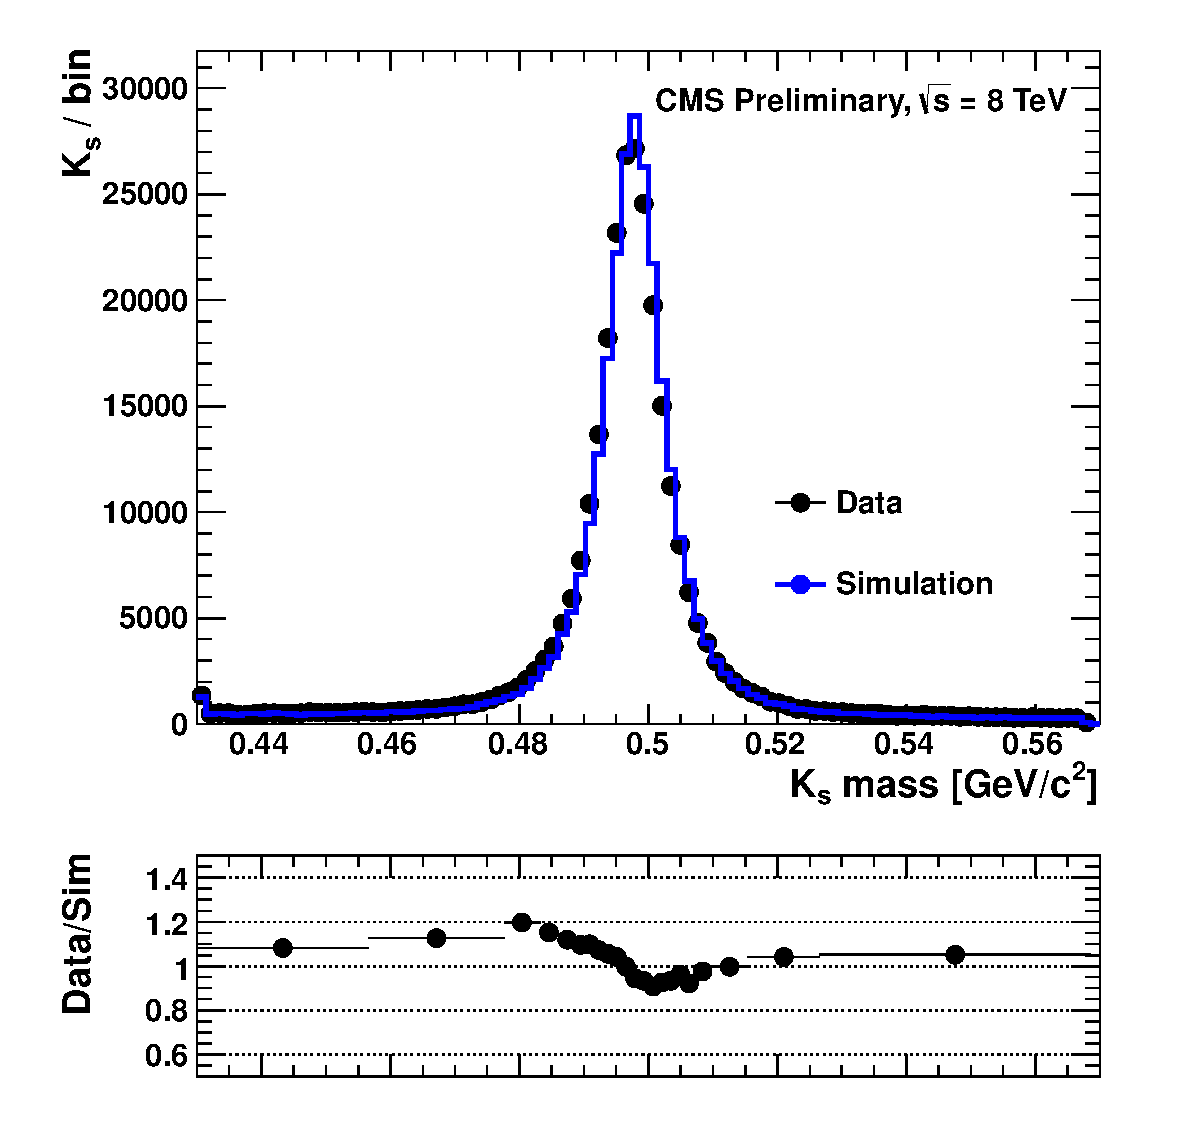
\includegraphics[width=0.49\textwidth]{plots/kshort/ksmass.pdf}
\caption{Invariant mass distribution of the \Kshort candidates in data and simulation. \label{fig:ksmass}}
\end{figure} 


The mean lifetime of the \Kshort is known with better than 0.1\% precision, however the \Kshort
production rate as well as its kinematic distributions are not perfectly reproduced 
by \PYTHIA \cite{Khachatryan:2011tm}.
In order to remove a potential bias arising from the generator level discrepancies, 
we select the \Kshort candidates with transverse decay length $L_{xy}<2\cm$ where tracking efficiency
is high and well simulated. We then compare $p_T$ and $\eta$ distributions for these candidates and obtain
weights, binned in $p_T$ and $\eta$, as well as an overall scale factor which are further
 applied for all \Kshort candidates. 

\begin{figure}[htbp]
\centering
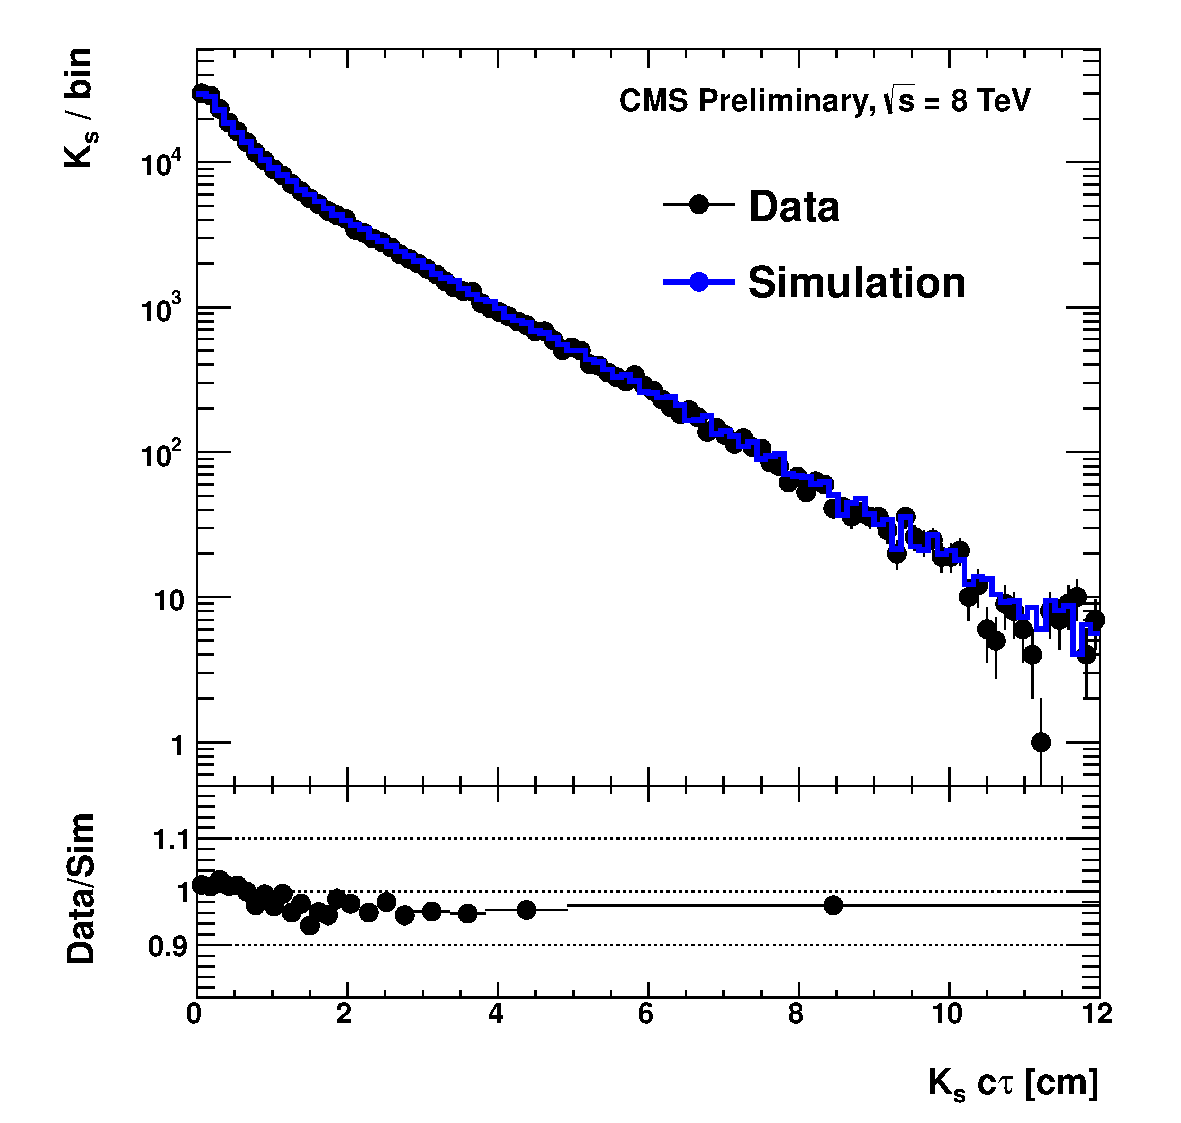
\includegraphics[width=0.49\textwidth]{plots/kshort/ksctau.pdf}
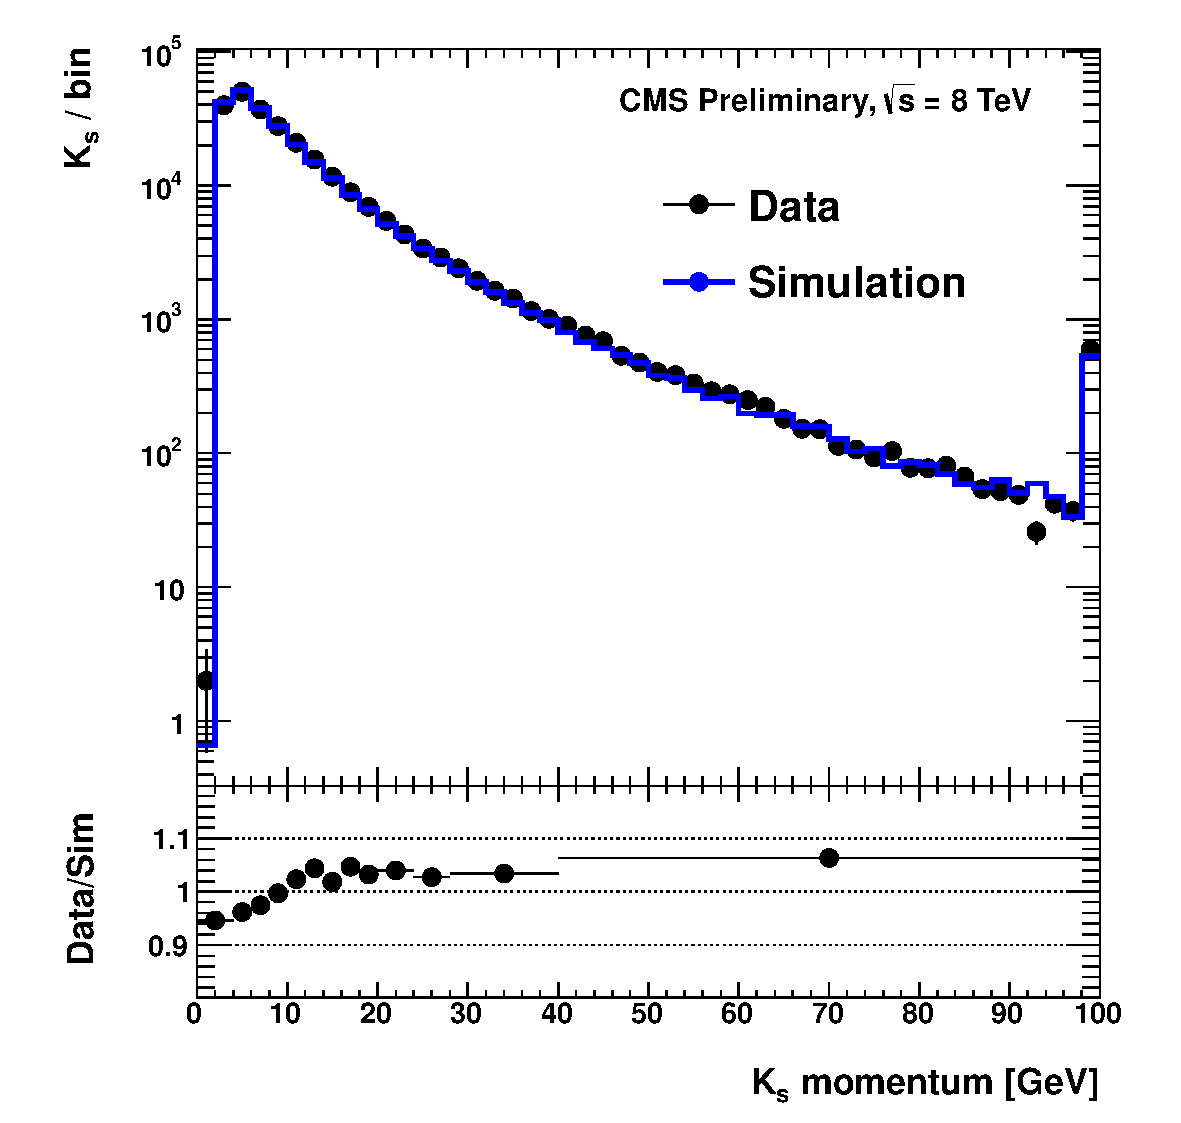
\includegraphics[width=0.49\textwidth]{plots/kshort/ksp.pdf}
\caption{Proper lifetime and momentum distributions of the \Kshort candidates in data and simulation. \label{fig:ksctau}}
\end{figure}

The proper lifetime and momentum distributions of the \Kshort candidates are
shown in Figure \ref{fig:ksctau}, while
Figure \ref{fig:ksdisplacement} shows the two and three dimensional decay lengths and track impact
 parameter distributions for data and simulation.  
 A good agreement between data and simulation is found, with simulation
 deviations not exceeding 10\%.   

\begin{figure}[htbp]
\centering
\includegraphics[width=0.49\textwidth]{plots/kshort/kslxy.pdf}
\includegraphics[width=0.49\textwidth]{plots/kshort/kslxyz.pdf}\\
\includegraphics[width=0.49\textwidth]{plots/kshort/kstrkip2d.pdf}
\includegraphics[width=0.49\textwidth]{plots/kshort/kstrkip3d.pdf}\\
\caption{Two-dimensional (top-left) decay length, three-dimensional decay length (top-right), two-dimensional track impact parameter (bottom-left) and three-dimensional track impact parameter (bottom-right) distributions 
of the \Kshort candidates in data and simulation. \label{fig:ksdisplacement}}
\end{figure}

The average number of 
reconstructed \Kshort candidates as a function of pile-up is presented in Figure \ref{fig:kspileup}. 
The decrease of tracking efficiency is found to be faster in data compared to simulation, while the 
effect is not bigger than 5\%.

\begin{figure}[htbp]
\centering
\includegraphics[width=0.49\textwidth]{plots/kshort/effnPV.pdf}
\caption{Average number of reconstructed \Kshort candidates as a function of number of primary vertices in data and simulation. \label{fig:kspileup}}
\end{figure}

The \Kshort reconstruction efficiency is proportional to the single track reconstruction efficiency squared, 
therefore the deviations between data and simulation of \Kshort distributions can be translated to twice smaller 
deviations in the single track reconstruction efficiency. We conservatively adopt the largest deviation 
of 10\% as the systematic uncertainty on the \Kshort efficiency and therefore a 5\% systematic on the 
single track reconstruction efficiency. 

\subsection{Impact on the signal reconstruction efficiency}

We examine the effect of tracking efficiency systematic uncertainty by removing 5\% of the displaced tracks 
 and repeating the signal reconstruction procedure.
For all signal models the reconstruction efficiency is lowered by up to 4\% which we adopt as our reconstruction
efficiency systematic related to displaced tracking efficiency.  

\section{Track missing hits}

In the pre-selection criteria the tracks in the displaced dijet vertex are required to have on average
 less than 2 missing hits behind the vertex position. The efficiency of this requirement is above 98\% 
for the simulated signal dijets as shown in Table \ref{tab:seleff}. 
The number of missing measurements depends on the number of tracking modules which are capable of providing
valid hits along the path of each track, which may not be properly simulated as the overall number of 
not functional modules in data changes over the data taking period. We study the average number of missing
hits behind the vertex position in a control sample of prompt dijets in data and simulation. We apply the
analogous selection criteria which are applied to the signal dijets,
 while omitting the requirements on prompt tracks and vertex displacement. Figure \ref{fig:misshits} presents
the average number of missing hits behind the vertex position per track for prompt dijets in data and simulation.

\begin{figure}[htbp]
\centering
\includegraphics[width=0.49\textwidth]{plots/misshits/misshits.pdf}
\caption{Average number of tracker missing hits behind vertex position per track for prompt dijets
in data and simulation.\label{fig:misshits}}
\end{figure}

There are more missing hits observed in data, however the requirement of less than 2
missing hits on average is 98\% efficient in both data and simulation. Given the agreement in the efficiency
of this selection we do not assign additional systematic uncertainty. 

\section{Jet energy scale}
\label{sec:jessys}

In CMS reconstruction the jet energies are determined by applying a set of corrections.
 The systematic uncertainties on the corrections are also provided. The uncertainties vary as a function
 of jet $p_T$ and $\eta$ and are different depending on the jet algorithm \cite{Chatrchyan:2011ds}.
 Therefore, the effect of these
uncertainties on the signal reconstruction efficiency needs to be evaluated by applying variations to individual 
jets. In the event selection, described in Section \ref{sec:selection},
 we use the jet energy information in the following criteria:
\begin{itemize}
\item $H_T>$325\GeV - using jets with $p_T>$40\GeV and $|\eta|<3$;
\item $p_T>$60\GeV for both jets of the di-jet candidate - here jets within $|\eta|<2$ are used.  
\end{itemize}    

We determine the systematic uncertainty due to jet energy scale by shifting all relevant jet energies by 
their individual uncertainties up and down. 
%Additionally, we assume that uncertainties for the two  
% jet algorithms, ak5Calo and ak5PF, are correlated, 
%since they both use energy information from the calorimeters. 
The systematic 
difference in signal reconstruction efficiency upon jet energy scale variations is presented in Table
\ref{tab:jessys}. For \Higgs mass of 1000 \GeV the uncertainty is negligible, while for lower masses
of the \Higgs the systematic effect is below 5\%. 


%For mass of 400 \GeV the 
%difference between signal models with \X mass of 50 \GeV and 150 \GeV comes from the fact of overall 
%underestimation of the total $H_T$ for \X of mass 150 \GeV. The mean $H_T$ for this sample falls below 
%325 \GeV, which is used as an offline cut, therefore making the efficiency more sensitive to jet energy scale
%variations. The underestimation of jet energies for \X of mass 150 \GeV is due to the fact
%of signal jets being relatively wide. In such a scenario a 0.5 cone algorithm 
%does not contain all of the jet constituents, which results in an underestimate of its energy. 
%The effect of $H_T$ underestimation for \X mass of 150 \GeV does not depend on the \X particle mean lifetime.
 

\begin{table}[htbp]
\centering
\caption{Signal reconstruction efficiency relative bias ($\Delta\epsilon$) due to jet energy scale uncertainties. \label{tab:jessys}}
\begin{tabular}{llc}
\hline
$M_{\Higgs}$ [\GeV] & $M_{\X}$ [\GeV]  & $\Delta\epsilon$ \\
\hline
200 & 50 & 4.4\% \\
400 & 50 & 2.7\% \\
400 & 150 & 4.8\% \\
1000 & 150 & 0.03\% \\ 
1000 & 350 & 0.02\% \\
\hline
\end{tabular}
\end{table}

\section{Jet momentum bias}
\label{sec:ptbias}

\X boson jets originate at transversely displaced locations which leads to two effects that affect the jet 
momentum determination:
\begin{itemize}
 \item skewed approach angle at the calorimeters face. This effect is a result of the displacement 
of the jet production point combined with the opening angle of the $\qq$ pair.
If the angle is large, the jet particles pass sideways through the calorimeters 
 which results in a geometrical bias of the individual
particles momentum and therefore the entire jet momentum;  
 \item reduced tracking efficiency for tracks originating far from the interaction point. 
%This effect
%is applicable only to Particle Flow jets which employ the tracking information, while it is not relevant for the 
%Calo jets. 
In the jet reconstruction algorithm when charged particles
are not reconstructed as tracks, they are assumed to be neutral particles, therefore the jet 
charged energy fraction is underestimated in favor of the neutral energy fraction. 
The calorimeter response to charged and neutral particles is different,
therefore the mis-measured energy fractions lead to biased jet energy corrections.
\end{itemize}
Figure \ref{fig:jetbias} shows the bias (points) and the resolution (error bars) of the signal jets $p_T$  as a function of the \X boson transverse decay length $L_{xy}$.

\begin{figure}[htbp]
\centering
\includegraphics[width=0.99\textwidth]{plots/signal/biaslxy.pdf}
\caption{Signal jet $p_T$ bias and resolution as a function of the \X boson transverse decay length.\label{fig:jetbias}}
\end{figure} 
   
\begin{figure}[htbp]
\centering
\includegraphics[width=0.99\textwidth]{plots/signal/biasapproachAngle.pdf}
\caption{Signal jet $p_T$ bias and resolution as a function of the jet approach angle at the calorimeters.\label{fig:jetbiasAngle}}
\end{figure} 

The jet momentum bias due to geometrical displacement is found to be up to -10\% for dijet candidates with transverse
decay lengths below 60\cm, while it is small for the prompt jets as expected. The level of the bias differs
depending on the signal mass point chosen, while the variation is related to the calorimeter approach angle
which is influenced by the opening angle of the $\qq$ pairs.
The jet momentum bias as a function of the calorimeter approach angle is shown in Figure \ref{fig:jetbiasAngle}.
If the jet approach angle is restricted to below one degree, the jet momentum bias is found to be reduced by half.
 Therefore, the two effects related to tracking efficiency and skewed approach angle contribute to the 
momentum bias in approximately the same amounts.

We do not assign a systematic uncertainty related to the jet momentum bias arising from the skewed approach angle 
at the calorimeters under the assumption that the detector geometry is well described in the MC simulation.
In Section \ref{subsec:pitrkeff} we assign a 5\% systematic uncertainty on single track efficiency for 
displaced tracks. We therefore study a 5\% variation of the jet charged energy
fraction and its impact on the signal reconstruction efficiency with the results presented 
in Table \ref{tab:jetbias}. 
%The variation is relevant only for selection criteria where Particle Flow jets
%are used. 

\begin{table}[htbp]
\centering
\caption{Signal reconstruction efficiency bias upon a 5\% variation in the jet charged energy fraction.\label{tab:jetbias}}
\begin{tabular}{ccc}
\hline
  $M_{\Higgs}$ [\GeV] & $M_{\X}$ [\GeV] & $\Delta\epsilon$ \\
\hline
       ~200      &        50      &     4.9\%      \\
       ~400      &        50      &     4.5\%      \\
       ~400      &       150      &     3.6\%      \\
       1000      &       150      &     0.9\%      \\
       1000      &       350      &     0.5\%      \\
\hline
\end{tabular}
\end{table}

%\subsection{PDF systematics}
%\label{subsec:pdfsys}

%The signal Monte Carlo samples are generated using \PYTHIA. According to the recommendations on Parton Density
%Functions use at the LHC \cite{Bourilkov:2006cj}, the events are then re-weighted using 
%three PDF sets:
%\begin{itemize}
%\item CT10 - update of CTEQ6.6
%\item MSTW08
%\item NNPDF2.0
%\end{itemize}   
%The signal efficiency is calculated, where only kinematic selection criteria are applied, 
%namely the trigger, $p_T$ and pseudo-rapidity selections on
%the jets. These partial signal efficiencies are listed in Table \ref{tab:pdfsys}. Uncertainties on the efficiencies
% are determined from the systematic variation obtained with the listed PDF sets. 
%The relative uncertainty does
%not exceed 1\% for any considered signal model, therefore we adopt a 1\% systematic uncertainty as a conservative
%estimation of the PDF uncertainty for all signal models.
 

%\begin{table}[htbp]
%\centering
%\caption{Signal reconstruction efficiency for all simulated signal models, where only  the trigger, jet $p_T$ and 
%$\eta$ selections are applied. The uncertainties quoted on these numbers correspond to the systematic uncertainty on the PDF sets.\label{tab:pdfsys}}
%\begin{tabular}{llllc}
%\Higgs [GeV] & \X [GeV] & c$\tau$ [cm] & $\epsilon$ [\%] &  Relative Error [\%] \\
%\hline
%\hline
%200 & 50 & 2 & 2.3$\pm0.006$ & 0.3 \\
%200 & 50 & 20 & 3.1$\pm0.011$ & 0.4 \\
%\hline
%400 & 50 & 0.8 & 28.0$\pm0.19$ & 0.7 \\
%400 & 50 & 8 & 50.0$\pm0.4$ & 0.7 \\
%400 & 50 & 80 & 11.0$\pm0.11$ & 1.0 \\
%\hline
%400 & 150 & 4 & 38.0$\pm0.29$ & 0.8 \\
%400 & 150 & 40 & 43.0$\pm0.43$ & 1.0 \\
%400 & 150 & 400 & 9.3$\pm0.10$ & 1.0 \\
%\hline
%1000 & 150 & 1 & 75.0$\pm0.16$ & 0.2 \\
%1000 & 150 & 10 & 85.0$\pm0.30$ & 0.4 \\
%1000 & 150 & 100 & 23.0$\pm0135$ & 0.6\\
%\hline
%1000 & 350 & 3.5 & 91.0$\pm0.10$ & 0.1 \\
%1000 & 350 & 35 & 93.0$\pm0.11$ & 0.1 \\
%1000 & 350 & 350 & 34.0$\pm0.26$ & 0.8 \\
%\hline
%\end{tabular}
%\end{table}

%\section{Effect of higher-order QCD corrections}
%\label{sec:isr}

%As described in Section \ref{sec:jessys} the signal reconstruction efficiency is sensitive to the jet energy
%scale variations; in particular for signal models with \Higgs mass of 200 \GeV and 400 \GeV. 
%Therefore, the signal reconstruction efficiency is also sensitive to the modelling of
% the Higgs $p_T$ spectrum, which may be in turn influenced by higher-order QCD corrections. 
%To study this effect
%we re-weight the \PYTHIA \Higgs $p_T$ spectrum from our signal samples to match the corresponding distribution
%determined at NLO using \POWHEG \cite{Bagnaschi:2011tu}. For $M_{\Higgs}$ = 200 \GeV with $M_{\X}$ = 50 \GeV and for $M_{\Higgs}$ = 400 \GeV 
%with $M_{\X}$ = 150 \GeV signal models this changes the efficiency by 20\% and 3\% respectively, while for
%other signal models the corresponding change is below 1\%. 
%Since the hidden valley signature is used as a benchmark
%model, we do not incorporate this variation as an additional systematic uncertainty, but emphasize and quantify
%the sensitivity of the reconstruction efficiency to higher-order QCD corrections.  

\section{Trigger Efficiency}
\label{sec:trigeff}

The high level trigger used in the analysis, double displaced jet trigger described
in Section \ref{subsec:trigger}, has been emulated in all
 simulation samples. The trigger selection consists of several consecutive filters applied to each event, 
and the performance of each filter is studied individually in data and simulation with respect to 
the corresponding offline selection criteria. For studying each individual filter, events 
passing all trigger decisions 
are not used in order to avoid a possible bias with the signal sample. Individual filters and their efficiency are
described in the following sections.  

\subsection{Scalar sum of jets $E_T$}
\label{subsec:trigHT}
This trigger filter requires $H_T > $ 300\GeV. Its performance is studied using a lower threshold trigger which 
requires $H_T >$ 250\GeV. 
The lower threshold trigger has been heavily prescaled in 2012 LHC run, therefore the integrated luminosity corresponds to only 8\pbinv. 
In both trigger calculation and offline reconstruction, hadronic jets with $p_T>$40\GeV and $|\eta|<$3 are used
 for $H_T$ computation. 
Figure \ref{fig:effHT300} shows the trigger efficiency as a function of the offline $H_T$. 
The difference in performance between data and simulation can be inferred from the efficiency ratio 
shown at the bottom. The observed discrepancy in the turn-on curves close to the threshold is caused by the 
difference in Level 1 trigger seeds used in the simulation compared to data.
An offline selection on 
$H_T$ at 325\GeV is applied in the selection criteria. 
Above this value the differences in efficiency between data and simulation are up to
7\%. To account for these differences the simulation events are re-weighted to match the efficiency in data.
This re-weighting
lowers the signal efficiency by up to 2\% for all considered signal models. The systematic effects in the turn-on
curve shape are studied by re-weighting the simulation with data turn-on curves corresponding to
 different periods of the LHC data taking in 2012. The variations in efficiency are found consistent within 
less than 1\%, while we conservatively assign 1\% as a relative 
systematic uncertainty corresponding to this trigger filter.      

\begin{figure}[htbp]
\centering
 \includegraphics[width=0.49\textwidth]{plots/trigger/effHT300.pdf}
\caption{HLT\_HT300 trigger efficiency as a function of offline $H_T$ requirement. \label{fig:effHT300}}
\end{figure} 

\subsection{Two jets each with maximally 2 prompt tracks}
\label{subsec:trig2Trks}

This filter is analyzed with data passing the previous 
$H_T$ filter. Data collected by CMS with this filter applied has also been prescaled and 
amounts to 17\pbinv.  
While the filter in question
 requires at least two jets with $p_T>$ 60\GeV passing the requirement, it is sufficient to study
 only the efficiency
 of a single jet passing the filter with respect to number of prompt tracks computed offline.
 In both HLT trigger and offline
 reconstruction prompt tracks are selected as those with an impact parameter in 3 dimensions 
not bigger than 300$\mum$
 with respect to leading primary vertex. Figure \ref{fig:eff2Trks} shows the single jet efficiency of passing
 the requirement of maximally 2 prompt tracks as a function of the same variable computed offline.
 The trigger becomes efficient with number of offline prompt tracks less than 2. 
A drop in efficiency for 0 prompt tracks arises from a fact of different leading primary vertex assignment 
between HLT and offline reconstructions. 
In such a scenario a track may be assumed to be prompt at HLT and non-prompt
 in offline reconstruction or vice versa. 
  

\begin{figure}[htbp]
\centering
 \includegraphics[width=0.49\textwidth]{plots/trigger/effHT300_2Trk_NPromptTracks.pdf}
\caption{Single jet efficiency for jets having maximally of 2 prompt tracks as a function of number of offline prompt tracks. \label{fig:eff2Trks}}
\end{figure}

The trigger efficiency for jets passing the offline selection of maximally 2 prompt tracks 
is plotted in Figure \ref{fig:eff2Trksptetaphi}
 as a function of $p_T$, $\eta$ and $\phi$. In order to determine the differences in performance 
between data and simulation the efficiency ratios are fitted with a zeroth order polynomial for each variable.
The fits yield a value of 97\% consistent within statistical uncertainties in $p_T$, $\eta$ and $\phi$,
 however with the $\chi^2$ per degree of freedom of the fits up to 4. 
The statistical uncertainties on individual points in the ratio histograms
are thus inflated by a factor of 2 and the ratios refitted.
 The overall correction is determined from the average of the fit values for
$p_T$, $\eta$ and $\phi$ with the result of 97\%. The systematic uncertainty on the ratio 
is assigned as the maximal
difference between the fit values within their statistical uncertainties with the result of 0.6\%.
Therefore, we assign an overall correction of 97\% with a conservative 1\% systematic uncertainty for 
each jet passing this trigger filter. 
 
 
\begin{figure}[!h]
\centering
 \includegraphics[width=0.32\textwidth]{plots/trigger/effHT300_2Trk_Pt.pdf}
 \includegraphics[width=0.32\textwidth]{plots/trigger/effHT300_2Trk_Eta.pdf}
 \includegraphics[width=0.32\textwidth]{plots/trigger/effHT300_2Trk_Phi.pdf}
\caption{Single jet efficiency as a function of jet $p_T$, $\eta$ and $\phi$ for jets with maximally 2 offline prompt tracks. \label{fig:eff2Trksptetaphi}}
\end{figure}

\subsection{Two jets with maximally 15\% of energy fraction carried by prompt tracks}
\label{subsec:trig2PF}

Similarly, we require both filters from Sections \ref{subsec:trigHT} and \ref{subsec:trig2Trks} 
to accept the event and examine a single jet efficiency with respect to prompt charged energy
 fraction computed offline. In this trigger step the prompt tracks are defined
 as those having the transverse impact parameter not bigger than 500$\mum$. 
Using transverse impact parameter
minimizes the sensitivity to additional pile-up interactions in the event. The size of the luminous region in 
the transverse plane is very small, about 15$\mum$, therefore the track promptness definition is general
and does not depend on the choice of the leading primary vertex. 
Trigger efficiency as a function of prompt energy fraction computed offline is shown in Figure \ref{fig:eff2PF}.

\begin{figure}[htbp]
\centering
 \includegraphics[width=0.49\textwidth]{plots/trigger/effHT300_PF_PromptEnergyFrac.pdf}
\caption{Single jet efficiency for jets with maximally 15\% prompt energy fraction as a function of offline prompt energy fraction. \label{fig:eff2PF}}
\end{figure}     

Systematic differences between data and simulation are again studied after applying the offline selection at 15\%.
 The efficiency as a function of $p_T$, $\eta$, $\phi$ is presented in Figure \ref{fig:eff2PFptetaphi}. 
The same procedure as in Section 
\ref{subsec:trig2Trks} is followed and the efficiency ratios are fitted with a zeroth order polynomial.
 No error inflation is needed as the statistical uncertainties on the individual ratio bins are larger
due to limited statistics.
 We assign a correction of 97\% and a conservative systematic uncertainty of 2\% for
each jet passing this filter from the average and the spread of the fit results for $p_T$, $\eta$, and $\phi$.
Similar performance of the filters in Sections \ref{subsec:trig2Trks} and \ref{subsec:trig2PF} 
is expected since both filters use properties of the similar sets of tracks.

\begin{figure}[!h]
\centering
 \includegraphics[width=0.32\textwidth]{plots/trigger/effHT300_PF_Pt.pdf}
 \includegraphics[width=0.32\textwidth]{plots/trigger/effHT300_PF_Eta.pdf}
 \includegraphics[width=0.32\textwidth]{plots/trigger/effHT300_PF_Phi.pdf}
\caption{Single jet efficiency as a function of jet $p_T$, $\eta$ and $\phi$ for jets with maximally 15\% prompt energy fraction. \label{fig:eff2PFptetaphi}}
\end{figure}

\subsection{Overall trigger efficiency}

Each of the trigger filters have been analyzed individually by determining performance differences 
between data and simulation. Observable discrepancies are accounted for as corrections in Sections
 \ref{subsec:trig2Trks} and \ref{subsec:trig2PF} and the uncertainties on the corrections are treated as 
systematic uncertainties. The trigger used in the analysis requires
 at least two jets passing the filters from Sections \ref{subsec:trig2Trks} and \ref{subsec:trig2PF}, 
hence corrections need to be applied twice, while systematic uncertainties added as fully correlated. 
Additionally, systematic uncertainties related to filters from Sections 
\ref{subsec:trig2Trks} and \ref{subsec:trig2PF} are both related to reconstruction of prompt tracks, therefore
 we adopt a conservative approach and add them as correlated also. The systematic uncertainty assigned to 
the filter from Section 
\ref{subsec:trigHT} is related to the jets transverse energy, hence it can be treated as uncorrelated. 
The total correction applied to the per event trigger efficiency determined from simulation is thus 0.89 with a total
relative systematic uncertainty of 6\%. 

\section{Total signal efficiency systematic uncertainty}

Table \ref{tab:signalsystematics} summarizes the sources of systematic uncertainties on the signal efficiency. 
The various effects are assumed uncorrelated and therefore added in quadrature with the total
uncertainty between 8--10\% depending on the signal model.

\begin{table}[htbp]
\centering
 \begin{tabular}{r|l}
  Source & Uncertainty \\
  \hline
  Trigger efficiency & 6\% \\
  Tracking efficiency & 4\% \\
  Jet energy scale & 3-5\%(*) \\
  Jet momentum bias & 1-5\% \\ 
  %NLO effects & 3-20\%(*) \\ 
  Pile-up modelling & 2\% \\
%  Parton distribution functions & 1\% \\
  \hline
 Total & 8-10\% \\
 \end{tabular}
\caption{Summary of signal efficiency systematic uncertainties. *Applies only to samples with
 \Higgs mass of 200 and 400 \GeV.
\label{tab:signalsystematics}}
\end{table} 


\chapter{Results}
\section{Results}
\label{sec:results}

\subsection{X particles reconstruction efficiency}
\label{subsec:signalefficiency}

The signal events contain two \X bosons decaying to \qq, therefore we define the \X bosons 
 efficiency times acceptance ($\epsilon A$) as:
\begin{equation}
\epsilon A= \frac{N_{X reconstructed}}{2N_{events}}
\end{equation}

where the X bosons acceptance $A$ has been defined in Section \ref{subsec:sigsensitivity}. 
Table \ref{tab:sigeff} presents the acceptance and efficiency for
reconstructing \X boson candidates as a function of the \Higgs and \X particles masses for different 
mean lifetimes of the \X particles.

\begin{table}[htbp]
\caption{Signal reconstruction efficiency for individual $\X\rightarrow\qq$ decays in simulated signal models. 
Both trigger and reconstruction efficiency 
are included in the calculation. Uncertainties quoted on signal efficiencies are statistical only.\label{tab:sigeff}}
\centering
\begin{tabular}{lllll} 
\hline
$H^{0}$ [GeV] & $X$ [GeV] & c$\tau$ [cm] & Acceptance [\%] & $\epsilon$ [\%] \\
\hline
200 & 50 & 2 & $8.9\pm0.2$ & $1.5\pm0.3$ \\
200 & 50 & 20 & $7.2\pm0.2$ & $0.8\pm0.2$ \\
\hline
400 & 50 & 0.8 & $35.0\pm0.4$ & $8.9\pm0.4$ \\
400 & 50 & 8 & $31.0\pm0.4$ & $4.5\pm0.3$ \\
400 & 50 & 80 & $7.1\pm0.2$ & $1.6\pm0.4$ \\
\hline
400 & 150 & 4 & $59.0\pm0.4$ & $16.0\pm0.4$ \\
400 & 150 & 40 & $50.0\pm0.4$ & $6.9\pm0.3$ \\
400 & 150 & 400 & $13.0\pm0.3$ & $1.8\pm0.3$ \\
\hline
1000 & 150 & 1 & $73.0\pm0.4$ & $38.0\pm0.4$ \\
1000 & 150 & 10 & $66.0\pm0.4$ & $26.0\pm0.4$ \\
1000 & 150 & 100 & $15.0\pm0.3$ & $15.0\pm0.7$ \\
\hline
1000 & 350 & 3.5 & $87.0\pm0.3$ & $40.0\pm0.4$ \\
1000 & 350 & 35 & $76.0\pm0.3$ & $22.0\pm0.4$ \\
1000 & 350 & 350 & $19.0\pm0.3$ & $11.0\pm0.5$ \\
\hline
\end{tabular} 
\end{table}

\X particle reconstruction efficiencies presented in Table \ref{tab:sigeff} 
are applicable to a model where \X particles decay with equal branching fractions to u,d,s,c and b quark pairs.
Table \ref{tab:sigeffflavor} shows the \X particle reconstruction efficiencies separately for 
\X decaying light quarks (u,d,s) and
heavier quarks c and b. 


\begin{table}[htbp]
\caption{Signal reconstruction efficiency for individual $\X\rightarrow\qq$ decays
 in simulated signal models for light (uds) and heavy (c and b) quark flavors.
 Uncertainties quoted on signal efficiencies are statistical only.\label{tab:sigeffflavor}} 
\centering 
\begin{tabular}{llllll} 
\hline
$H^{0}$ [GeV] & $X$ [GeV] & c$\tau$ [cm] & $\epsilon_{uds}$ [\%] & $\epsilon_{c} [\%] $ & $\epsilon_{b}$ [\%]\\
\hline
200 & 50 & 2 & $1.9\pm0.4$ & $1.3\pm0.6$ & $0.5\pm0.4$ \\
200 & 50 & 20 & $0.92\pm0.3$ & $0.7\pm0.5$ & $0.5\pm0.4$ \\
\hline
400 & 50 & 0.8 & $10.0\pm0.5$ & $8.6\pm0.8$ & $4.2\pm0.6$ \\
400 & 50 & 8 & $5.3\pm0.4$ & $4.0\pm0.6$ & $2.5\pm0.5$ \\
400 & 50 & 80 & $1.9\pm0.5$ & $1.3\pm0.7$ & $0.92\pm0.6$ \\
\hline
400 & 150 & 4 & $18.0\pm0.5$ & $16.0\pm0.8$ & $11.0\pm0.7$ \\
400 & 150 & 40 & $7.5\pm0.4$ & $6.5\pm0.6$ & $5.4\pm0.5$ \\
400 & 150 & 400 & $2.1\pm0.4$ & $1.5\pm0.6$ & $1.2\pm0.5$ \\
\hline
1000 & 150 & 1 & $39.0\pm0.5$ & $39.0\pm0.9$ & $35.0\pm0.9$ \\
1000 & 150 & 10 & $26.0\pm0.5$ & $26.0\pm0.9$ & $25.0\pm0.9$ \\
1000 & 150 & 100 & $15.0\pm0.9$ & $16.0\pm2.0$ & $13.0\pm1.0$ \\
\hline
1000 & 350 & 3.5 & $41.0\pm0.5$ & $40.0\pm0.9$ & $36.0\pm0.8$ \\
1000 & 350 & 35 & $23.0\pm0.5$ & $22.0\pm0.8$ & $21.0\pm0.8$ \\
1000 & 350 & 350 & $12.0\pm0.7$ & $11.0\pm1.0$ & $9.4\pm1.0$ \\
\hline
\end{tabular} 
\end{table}

\begin{figure}[htbp]
\centering
\includegraphics[width=0.49\textwidth]{plots/signal/effNLepb.pdf}
\includegraphics[width=0.49\textwidth]{plots/signal/effBlxyzb.pdf}
\caption{$\X\rightarrow b\bar{b}$ reconstruction efficiency as a function of the total number of leptons 
originating from B mesons/baryons (left) and as a function of B mesons/baryons decay length. Only selected 
mass points are shown. The samples correspond to the mixture of the three generated mean 
lifetimes of the \X bosons. \label{fig:effb}}
\end{figure}

The c and b quarks hadronize mostly into D or B mesons respectively.
 Unlike the light quark mesons a significant fraction of heavy flavor
mesons decays semi-leptonically reducing the track multiplicity of the jets and also reducing the jet momenta
 due to the missing energy of associated neutrinos. 
Additionally the D or B mesons split the dijet vertex due to their intrinsic lifetime.
Figure \ref{fig:effb} shows the reconstruction efficiency of the $\X\rightarrow b\bar{b}$ candidates as a function
of the total number of leptons originating from the $b\bar{b}$ pair and as a function of the B mesons decay
length. The reconstruction efficiency is affected mostly by the number of leptons, while the dependence on the
B mesons decay length is much smaller.

In order to visualize the capabilities of the CMS detector for reconstructing long-lived particles decaying to 
dijets, 
the reconstructed dijet mass and $L_{xy}$ distributions for selected signal models are shown in Figure
\ref{fig:signal}. We assume the cross-section of the $\Higgs\rightarrow2\X$ process to be 1 pb and the branching 
ratio to quarks ($\X\rightarrow\qq$) to be 100\%.

\begin{figure}[htbp]
\centering
\includegraphics[width=0.49\textwidth]{plots/signal/mass.pdf}
\includegraphics[width=0.49\textwidth]{plots/signal/Lxy.pdf}
\caption{The reconstructed dijet mass and $L_{xy}$ for selected signal models; central lifetime out of the three available is presented.\label{fig:signal}}
\end{figure}

\subsection{Data in the signal region}
\label{subsec:fullunblinding}

Table \ref{tab:fullunblinding} summarizes the observed candidate counts in the signal region for the optimized 
selections detailed in Section \ref{subsec:cutvalues}. Data is found in good agreement with the 
background only hypothesis. In addition, the two selected candidates are examined using event displays
and are found consistent with background candidates as described in Figure \ref{fig:eventDisplays}.  

\begin{table}[htbp]
\centering
\begin{tabular}{|l|c|c|}
\hline
$\bf L_{xy}$ \bf selection & \bf low & \bf high \\
\hline
\bf Predicted Background & $ 1.60\pm0.58(stat+sys)$ & $ 1.14\pm0.54(stat+sys)$ \\
\hline
\bf Observed candidates & 2 & 1 \\ 
\hline
\end{tabular}
\caption{Observed candidates and predicted background for the optimized selections.\label{tab:fullunblinding}}
\end{table}

\begin{figure}
\centering
\includegraphics[width=0.495\textwidth]{plots/displays/ev1_vtx.png}
\includegraphics[width=0.495\textwidth]{plots/displays/ev2_vtx.png}

\caption{Event displays of the two candidates passing the optimized selection where only the selected di-jet pair
 (yellow cones) and 
the tracks associated to the displaced vertex (black lines) are shown, other objects being removed. 
Candidate 1 (left) with dijet invariant mass of 770 \GeVcc, which 
passes only the {\it low $L_{xy}$} selection, 
contains a secondary vertex, displaced transversely by 5 \cm, containing 5 tracks from one jet and 1 track
from the other. The 5 track vertex is consistent with a vertex of a B meson with invariant mass below 5 \GeVcc.
Candidate 2 (right) with dijet invariant mass of 75\GeVcc, 
which passes both {\it low} and {\it high $L_{xy}$} selections, contains a secondary vertex
, displaced transversely by 44 \cm, containing 5 tracks where 2 of these tracks are
associated to both jets due to the jets being nearby. The vertex invariant mass is low and its position
 coincides with one of the silicon 
tracker layers being consistent with a nuclear interaction vertex. \label{fig:eventDisplays}}
\end{figure} 



\subsection{Limits}
\label{subsec:limits}

Given the null result of the search an upper limit is quoted on the cross-section 
to produce $\Higgs\rightarrow \X\X$ times the branching ratio squared, $B^2$, for \X to decay into \qq. 
The expected number of signal dijet candidates passing the selection cuts can be expressed as:
\begin{equation}
N_X \geq 2 \mathcal{L}\epsilon A\sigma B^2
\end{equation}
where $\mathcal{L}$ is the integrated luminosity, $A$ is the acceptance,
 $\epsilon$ is the efficiency to reconstruct \X boson candidates
(Table \ref{tab:sigeff}), $\sigma$ is the production cross-section of the heavy resonance decaying to \XX and 
$B$ is the branching ratio of \X to dijets. The non-equality arises from the fact that when the branching ratio $B$
is smaller than 1, there is an additional contribution from events where only one \X boson decayed to dijets. 
The limits will therefore be exact when $B=1$ and conservative when $B$ is smaller than 1.
 

For each combination of the \Higgs and \X boson masses that are modelled and for a range of \X boson lifetimes,
the 95\% CL upper limits on $\sigma B^2$ are calculated.
  
%The lifetime re-weighting procedure is explained in Appendix \ref{sec:reweighting}.
 The limit calculation employs CL$_s$ method \cite{Read:2002hq} for a counting
experiment with 95\% confidence level. The calculation uses the statistics software 
package {\tt RooStatsCL95} recommended by
 the CMS Statistics Committee \cite{RooStatsCL95}. 

In order to expand the number of tested models
the lifetime distributions of the signal MC events are re-weighted to different
mean values using generator level lifetimes, thus providing additional signal efficiencies. 
%The lifetime re-weighting procedure is explained in Appendix \ref{sec:reweighting}.
The limits on $\sigma B^2$ and the limits on $\sigma B^2 A$ corrected for detector acceptance are computed. 
They are presetned in Figures
\ref{fig:limits} and \ref{fig:limitsacceptance} respectively.

\begin{figure}[htbp]
\centering
\includegraphics[width=0.49\textwidth]{plots/limits/1000_350e.pdf}
\includegraphics[width=0.49\textwidth]{plots/limits/1000_150e.pdf} 
\includegraphics[width=0.49\textwidth]{plots/limits/400_150e.pdf}
\includegraphics[width=0.49\textwidth]{plots/limits/400_50e.pdf} 
\includegraphics[width=0.49\textwidth]{plots/limits/200_50e.pdf}

\caption{Expected and observed 95\% CL limits for all tested signal models.\label{fig:limits}}
\end{figure}

\begin{figure}[htbp]
\centering
\includegraphics[width=0.49\textwidth]{plots/limits/1000_350ea.pdf}
\includegraphics[width=0.49\textwidth]{plots/limits/1000_150ea.pdf} 
\includegraphics[width=0.49\textwidth]{plots/limits/400_150ea.pdf}
\includegraphics[width=0.49\textwidth]{plots/limits/400_50ea.pdf} 
\includegraphics[width=0.49\textwidth]{plots/limits/200_50ea.pdf}

\caption{Expected and observed 95\% CL limits within the detector acceptance for all tested signal models.\label{fig:limitsacceptance}}
\end{figure}

\subsection{Conclusions}
\label{subsec:conclusions}

For pp collisions at $\sqrt{s}=8 \TeV$, upper limits are placed on the production cross section
of a heavy resonance decaying to two long-lived, spin 0, neutral particles \X, where the massive resonance
is taken to be a Higgs boson, times the branching ratio squared of $\X$ decaying to \qq, where $q$ denotes any
of the $u,d,s,c,b$ quark flavors. For Higgs masses of 200-1000\GeVcc and \X boson masses of 50-350\GeVcc,
these limits are typically in the range 0.0005-0.3 $pb$, for \X bosons whose lifetime is such their mean 
transverse decay length is less than about 1 metre.     


\chapter{Conclusions}
%\input Conclusion.tex


\appendix
\chapter{Hierarchical Clusters}

% Say what the application is
In this analysis dijet tracks are clustered, using a method known as {\it hierarchical clustering}, according to 
their $L_{xy}^\text{exp}$ as described in Section \ref{subsec:Clusters}.

Hierarchical clustering connects elements of an unclustered set using a similarity (linkage) criterion,
as shown schematically in Figure \ref{fig:dendrogram}.
\begin{figure}[htbp]
\centering
\includegraphics[width=0.5\textwidth]{plots/dendrogram2.png}
% correct the plot
\caption{Dendrogram presenting hierarchical clustering. \label{fig:dendrogram}}
\end{figure}

 Initially each element is its own cluster (A-G). Each of the next steps merges 
the two most similar clusters into one.
In the case of clustering numbers the similarity criterion is the smallest distance 
between clusters. For clusters A and B the similarity is obtained as follows:
\begin{equation}
\min \{\, d(x,y) : x \in \mathcal{A},\, y \in \mathcal{B} \,\}, \hspace{5pt} d(x,y)=|x-y| 
\label{eqn:linkage}
\end{equation}
where $\mathcal{A}$ and $\mathcal{B}$ are already existing clusters.
 As presented in Figure \ref{fig:dendrogram} the first step connects clusters B and C, the second step connects clusters D and E, etc.
The procedure is repeated until the similarity criterion is no longer satisfied. In Figure \ref{fig:dendrogram} the minimal similarity criterion is 
schematically presented as a horizontal
dashed line. The clustering procedure results in two clusters: ABC and DEFG. In the dijet analysis we cluster tracks according to 
their $L_{xy}^\text{exp}$ only, if the minimal distance between the clusters (Eqn. \ref{eqn:linkage}) does not exceed 15\% of the secondary vertex $L_{xy}$.


\chapter{Impact of the signal efficiency systematic uncertainty on the expected limit}

The impact of the signal efficiency systematic uncertainty on the expected limit is studied. 
The luminosity and background predictions together with their uncertainties are fixed to the ones used 
in this analysis, while the signal efficiency and its relative uncertainty are varied.


\begin{figure}[htbp]
\centering
\includegraphics[width=0.45\textwidth]{plots/degradation/10percent.pdf}
\includegraphics[width=0.45\textwidth]{plots/degradation/1percent.pdf}
\caption{Expected limit degradation as a function of signal efficiency systematic uncertainty.
The signal efficiency central value is assumed to be 10\% (left) and 1\% (right). A second order polynomial
is fitted to the expected limit graph with the fit parameter values listed in the legend.\label{fig:degradation}}
\end{figure}

Figure \ref{fig:degradation} shows the relative expected limit and 1$\sigma$ band degradation as the 
systematic uncertainty on signal efficiency is varied from 0 to 90\%. The degradation of the limit does not depend
on the central value of the efficiency itself. Relative to a limit obtained with no uncertainty, a 
degradation of 10\% is observed for a 30\% the systematic uncertainty. The limit degradation has also been studied 
assuming Gaussian or Log-normal parametrizations of the nuisance parameters yielding similar results.

In this analysis the systematic uncertainty on the signal efficiency has been conservatively 
estimated to at most 10\% for all signal models considered. A precise estimate of its value is of secondary importance given a small impact on the resulting limit.
      


\cleardoublepage 
\bibliographystyle{ieeetr}  %or your favorite style plain/abbrv/alpha/unsrt/acm/apalike
\bibliography{thesis}  %assuming your bibtex file is thesis.bib
\end{document}
